\documentclass[conference]{IEEEtran}

\usepackage{blindtext}
\usepackage{graphicx}
\usepackage{hyperref}
\usepackage{float}
%\usepackage{caption}
%\usepackage{subcaption}

\usepackage{cite}
% Loading the cite package will
% result in citation numbers being automatically sorted and properly
% "compressed/ranged". e.g., [1], [9], [2], [7], [5], [6] without using
% cite.sty will become [1], [2], [5]--[7], [9] using cite.sty. cite.sty's
% \cite will automatically add leading space, if needed. 

% correct bad hyphenation here
\hyphenation{op-tical net-works semi-conduc-tor}


\begin{document}

% can use linebreaks \\ within to get better formatting as desired
\title{StudyPal: A Website for Study Groups}

\author{\IEEEauthorblockN{James Beavers}
\IEEEauthorblockA{Department of Computer Science\\
North Carolina State University\\
Raleigh, North Carolina, USA\\
jjbeaver@ncsu.edu}
\and
\IEEEauthorblockN{Anthony Elliott}
\IEEEauthorblockA{Department of Computer Science\\
North Carolina State University\\
Raleigh, North Carolina, USA\\
anthony\_elliott@ncsu.edu}}


\maketitle


\begin{abstract}
Current university students form study groups with peers to help prepare for exams or work through assignments together.
Students often form study groups only with people they know very well from face-to-face contact.
We developed a prototype website called StudyPal to facilitate the creation and organization of study groups.
We predict how long experts should take to complete three primary tasks within StudyPal using the Keystroke-Level Model and conducted an empirical evaluation of 4 people to assess the accuracy of the predictions.
\end{abstract}

\IEEEpeerreviewmaketitle



\section{Introduction}
StudyPal is a website we designed and created to help university students form study groups for their classes.

%todo: might be better to merge these subsections later, I created them just to make sure I got everything

\subsection{Task Domain}
Students often form study groups for a specific class in which they help each other with exam preparation, readings, or assignments.
These study groups are formalized meetings set up ahead of time, in contrast to unplanned meetings.
Meeting length can vary from one hour to several hours.
Group sizes are typically small, with 2-5 participants.
Groups often consist of systematically going through a study guide for the class, either provided by the class instructor or created by the group participants.


\subsection{Target Users}
StudyPal is intended for use by both undergraduate and graduate students at North Carolina State University (NCSU).
If successful at NCSU then we plan to extend StudyPal to students at other universities.
StudyPal currently only uses the English language and thus only expected to be used by English-speaking students.


\subsection{Representative Scenarios}

In preparation for carrying out these tasks, our system assumes the user has created a Google calendar named 'class\_schedule' and it has been marked as public.  While a user can carry out all relevant tasks without having completed this step, it does take away from the user experience in some ways.  The user's schedule will not appear in the calendar view of the group info pages. As a result, members of the group will be unable to see that user's schedule and it could make scheduling meetings a bit more difficult. This is a limitation, but it isn't terribly far-fetched since maintaining a calendar for courses and academic-related work as a student seems reasonable.  However, this is a component of the system which we would like to revisit in future versions of the system.  Ideally the user would be able to specify a calendar name, for example.

\begin{figure}[ht!]
\centering
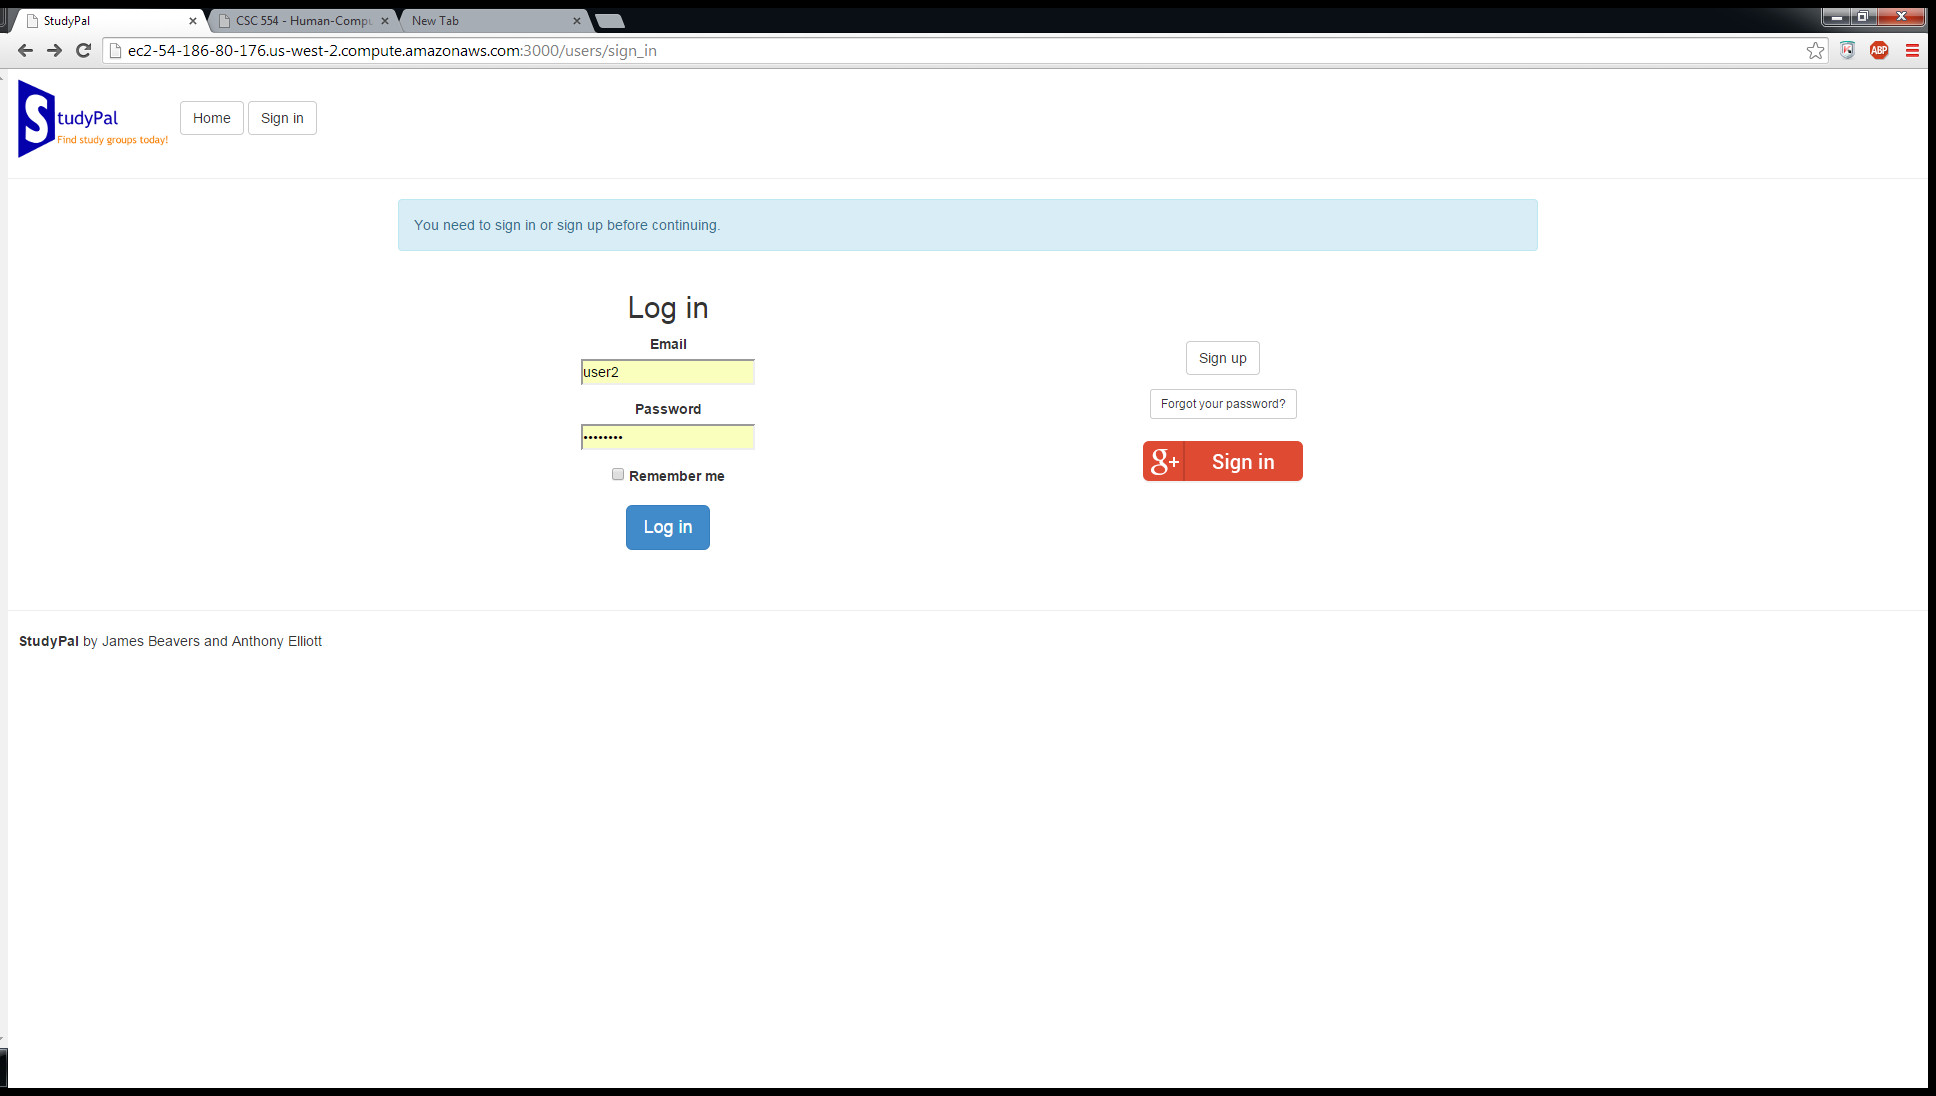
\includegraphics[width=80mm]{figures/login}
\caption{Login Screen \label{fig:login}}
\end{figure}

\subsubsection{Joining a Group}
Users enter the website (figure~\ref{fig:login}) and enter their user information to create an account (figure~\ref{fig:userInfo}). 

\begin{figure}[ht!]
\centering
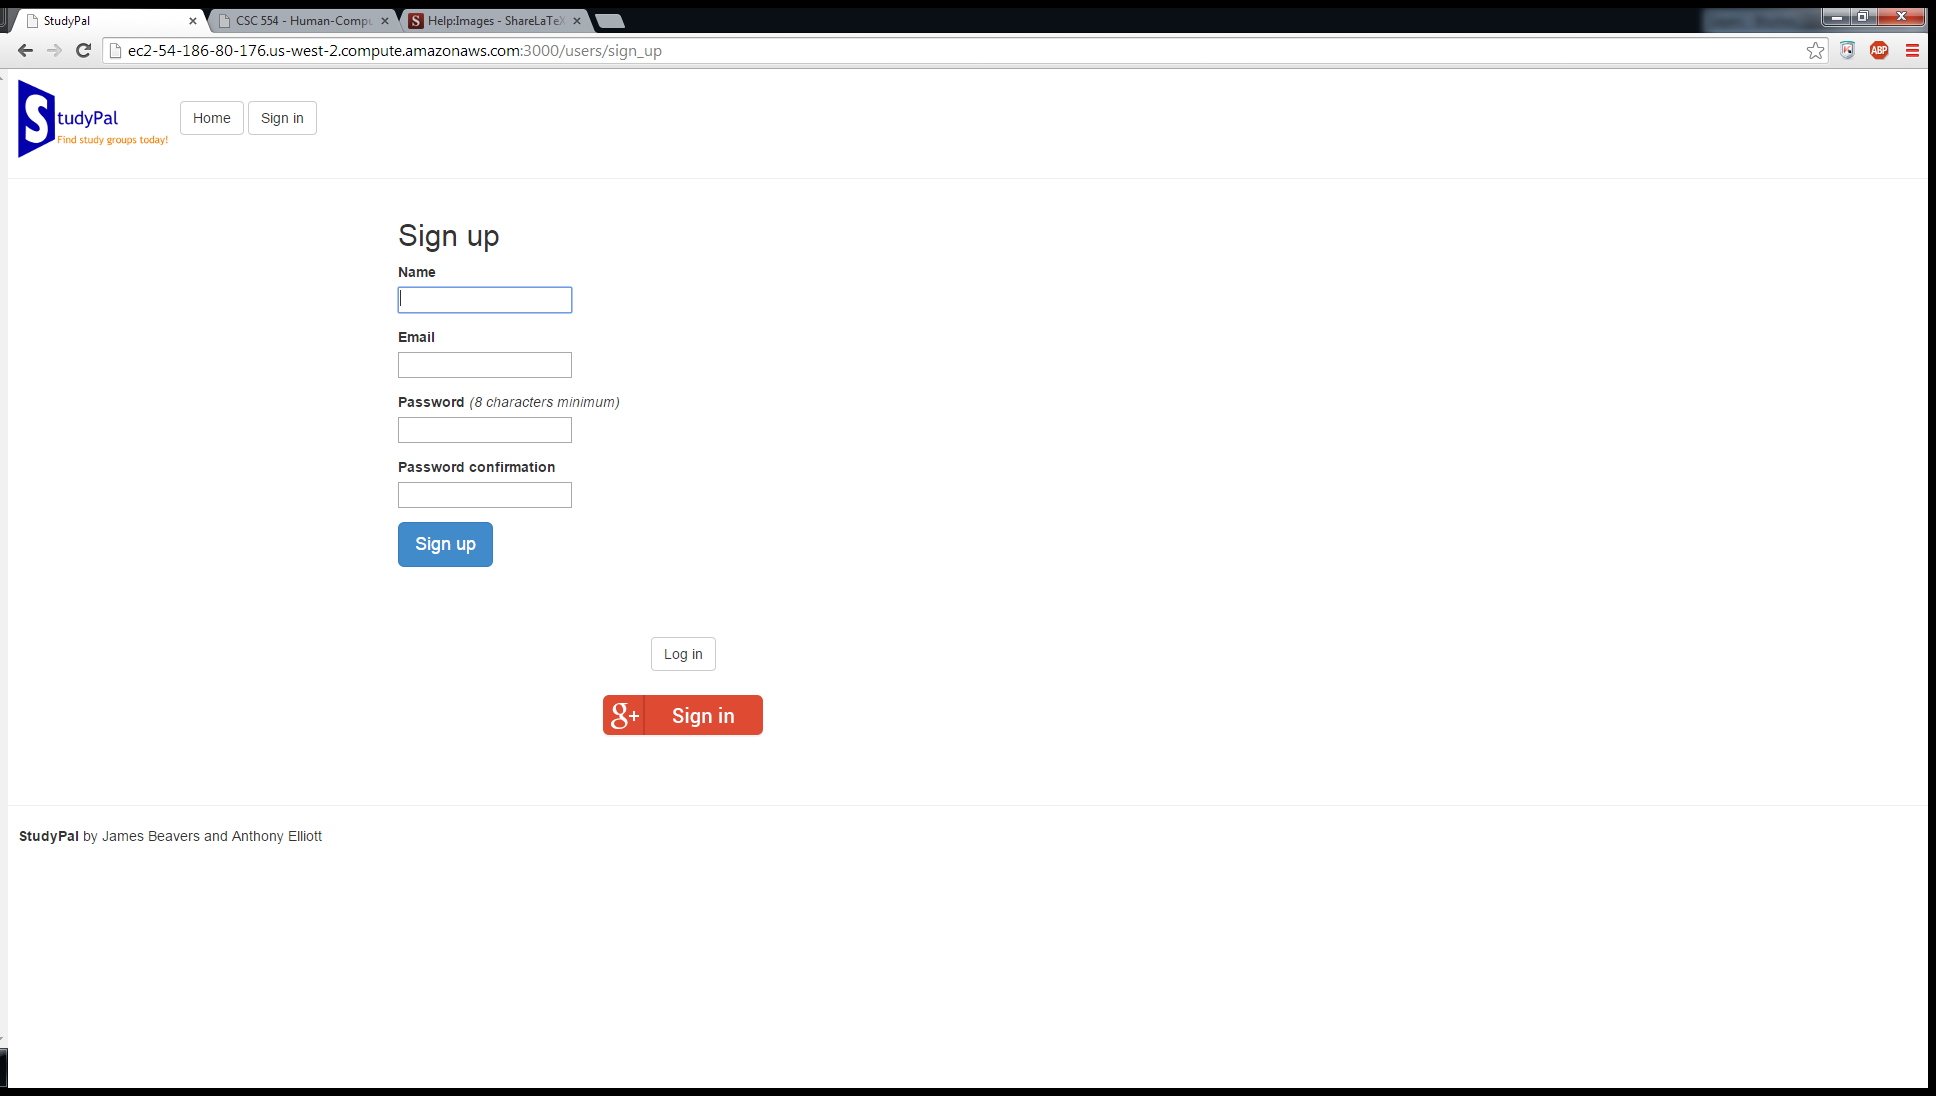
\includegraphics[width=80mm]{figures/userInfo}
\caption{User Info \label{fig:userInfo}}
\end{figure}

Alternatively, the user may log in using their Google account and password (figure~\ref{fig:oauth1} and~\ref{fig:oauth2}).  This is the method that our users were asked to do while completing these representative tasks.

\begin{figure}[ht!]
\centering
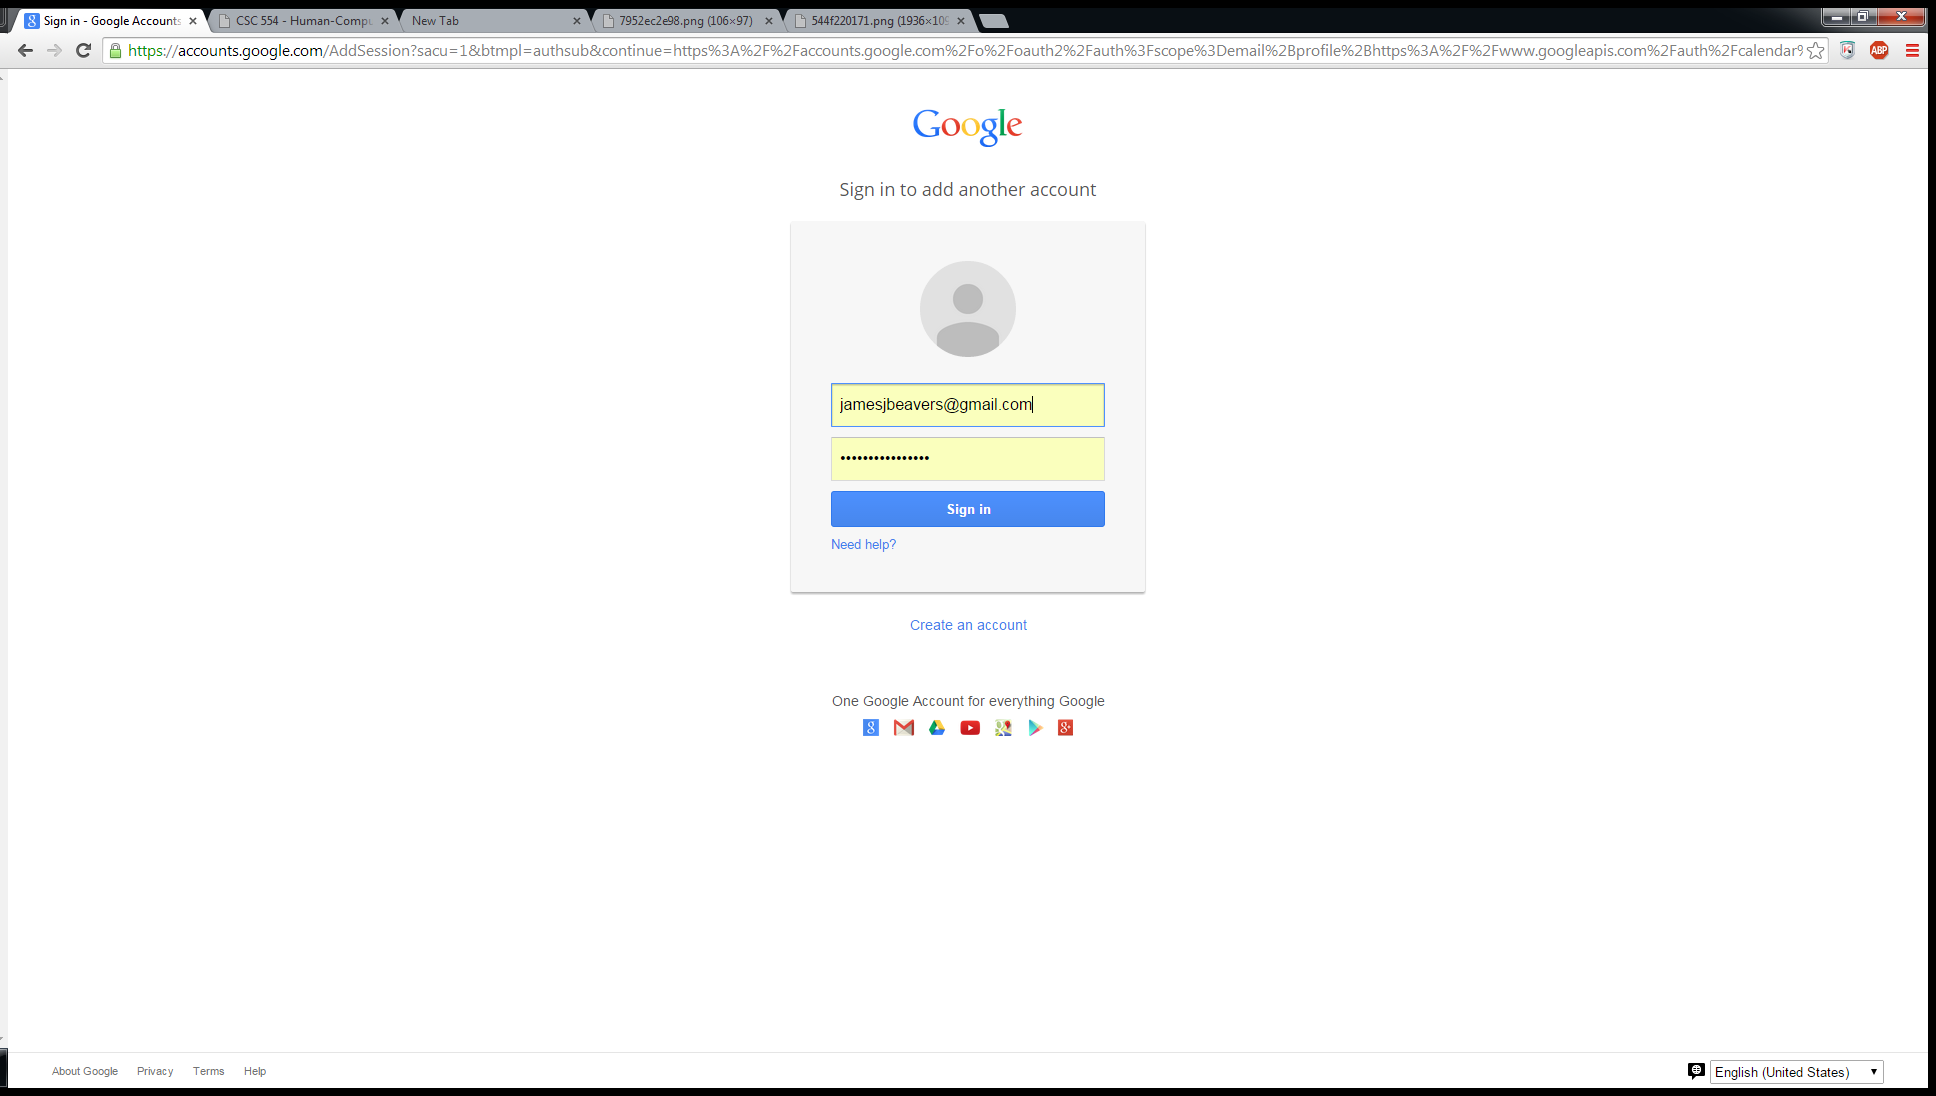
\includegraphics[width=80mm]{figures/oauth1}
\caption{Google Login 1 \label{fig:oauth1}}
\end{figure}

\begin{figure}[ht!]
\centering
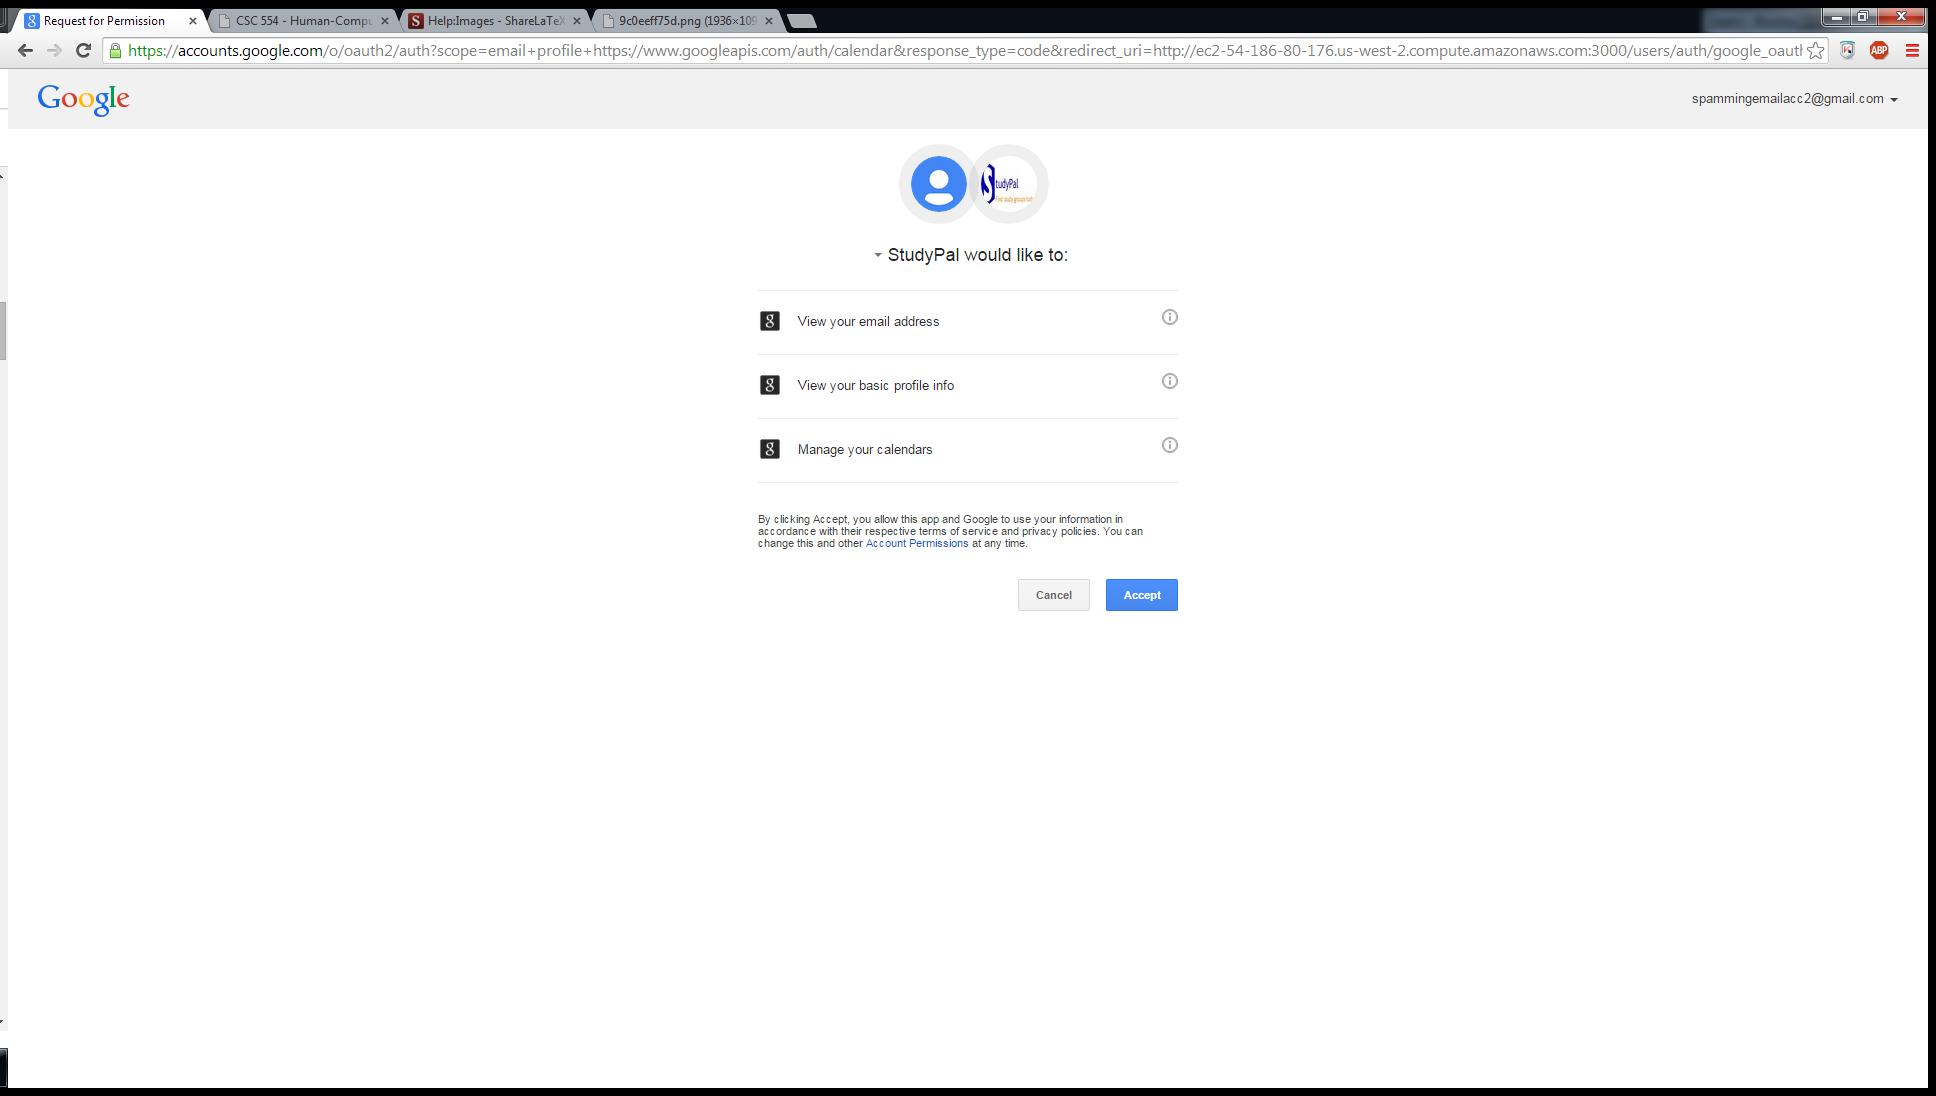
\includegraphics[width=80mm]{figures/oauth2}
\caption{Google Login 2 \label{fig:oauth2}}
\end{figure}

After logging in to the website, the user may immediately begin exploring groups, or he/she may enter their qualifications on the profile page (accessible via the header) (figure~\ref{fig:profile}).

\begin{figure}[ht!]
\centering
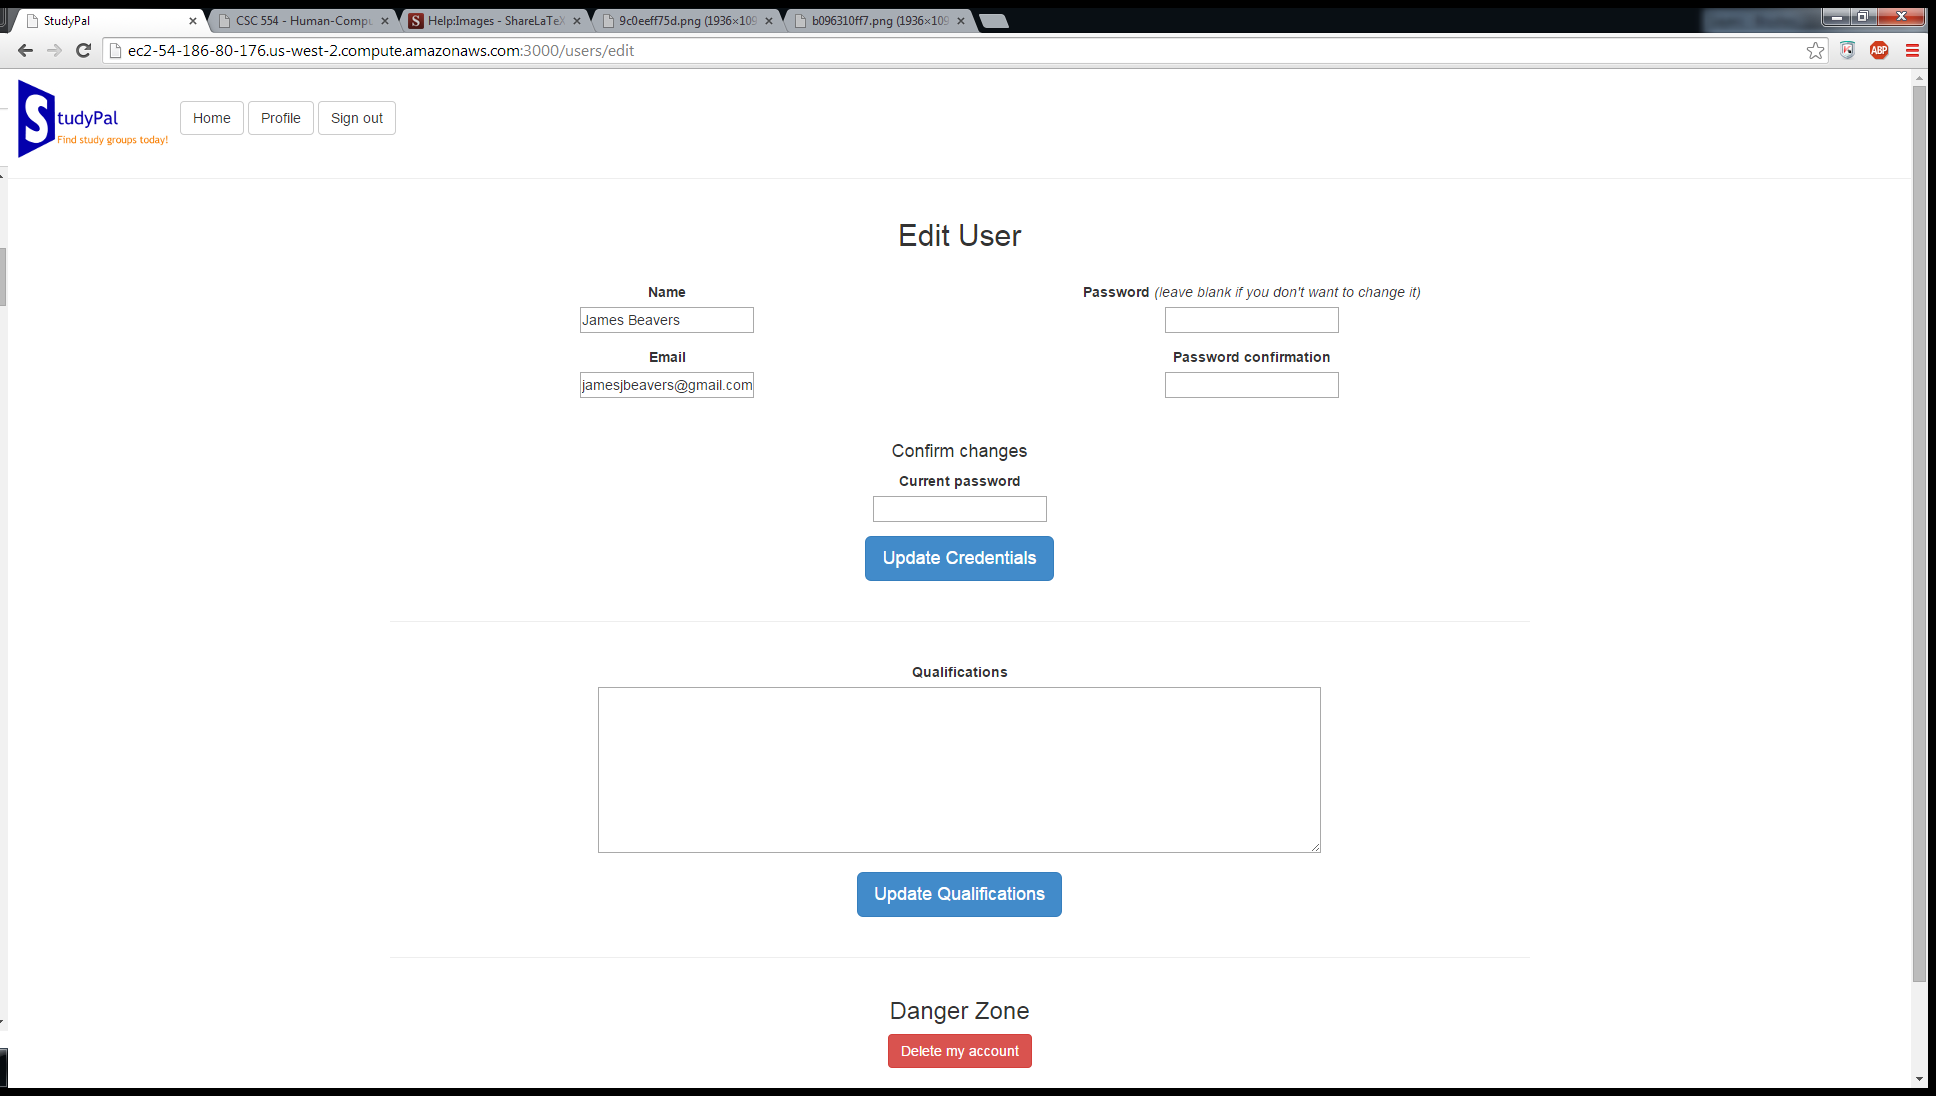
\includegraphics[width=80mm]{figures/profile}
\caption{User Profile \label{fig:profile}}
\end{figure}

Once the user has entered qualifications, he or she selects 'Explore Groups' to see a list of all study groups (figure~\ref{fig:home} and~\ref{fig:groupList}). 

\begin{figure}[ht!]
\centering
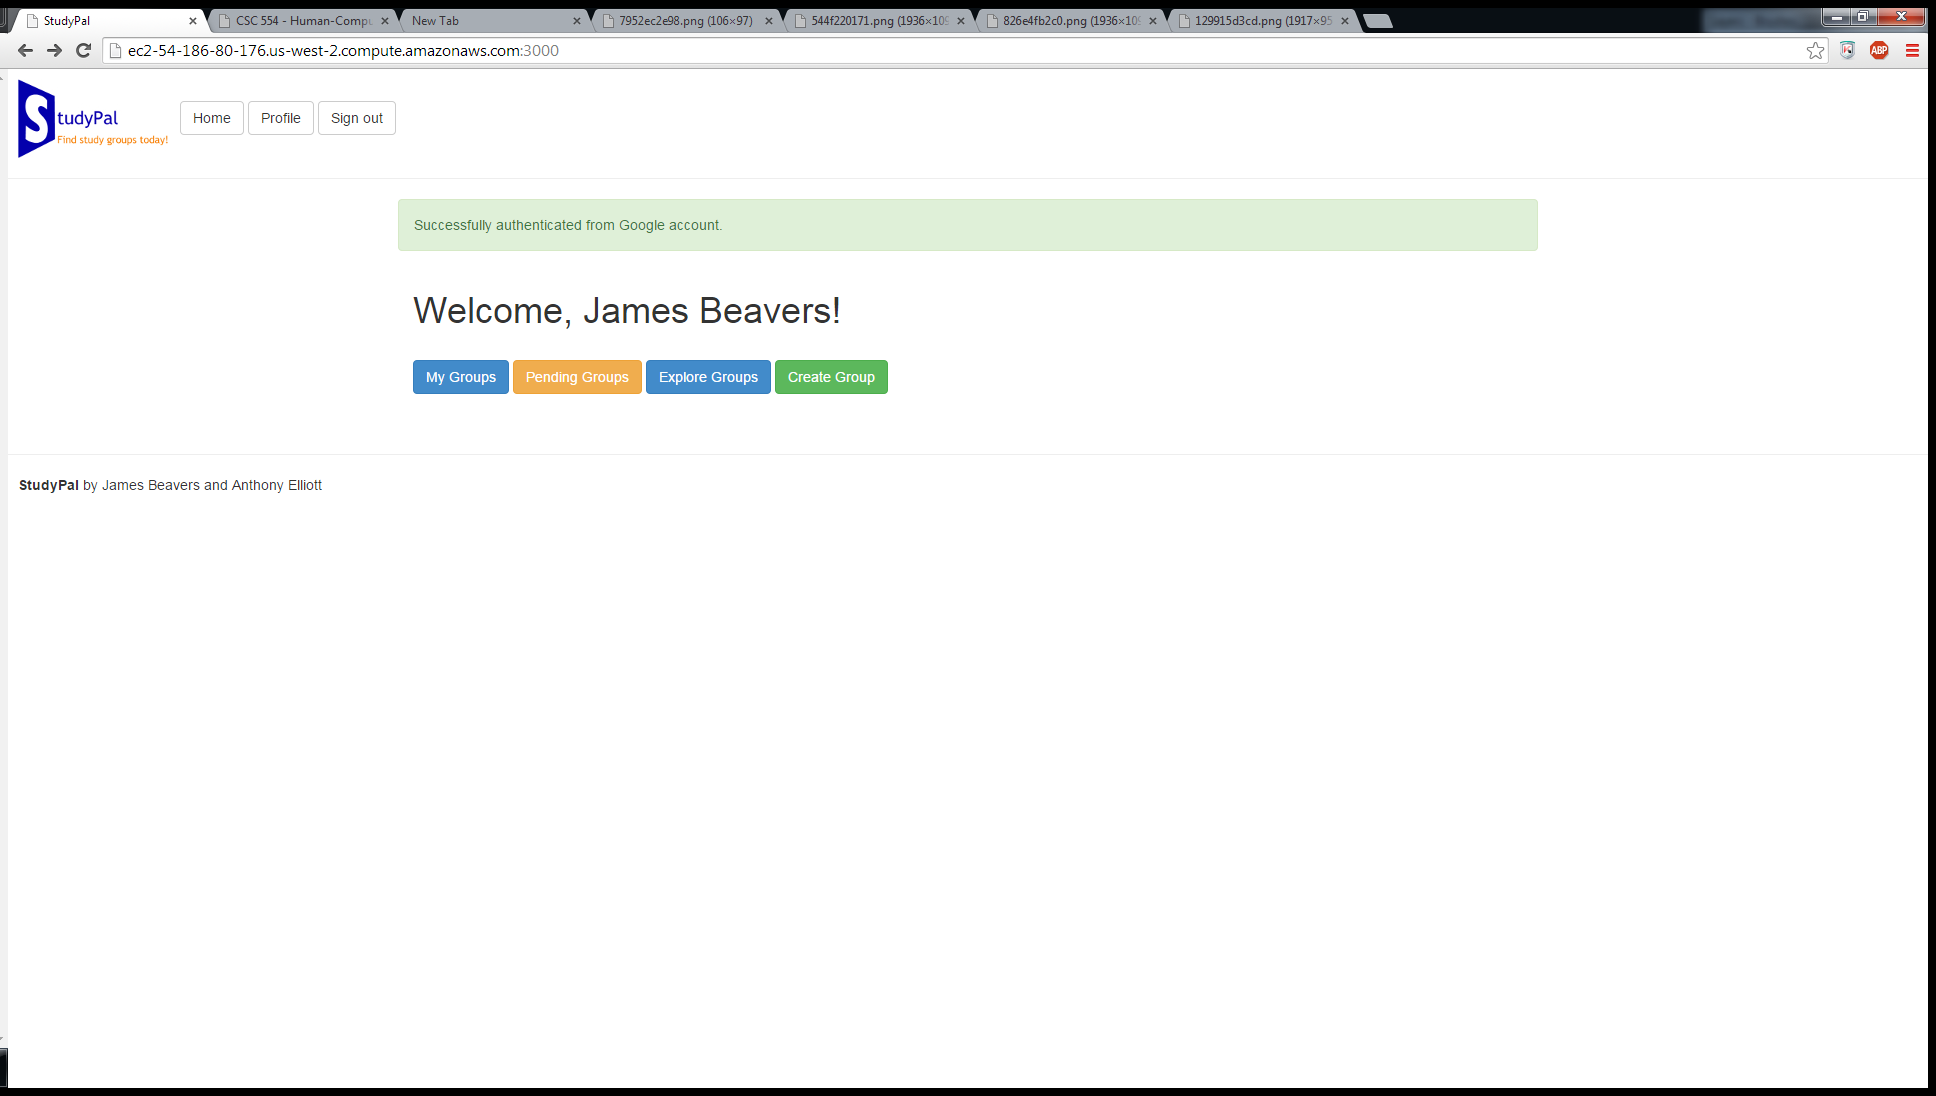
\includegraphics[width=80mm]{figures/home}
\caption{Home Screen \label{fig:home}}
\end{figure}

\begin{figure}[ht!]
\centering
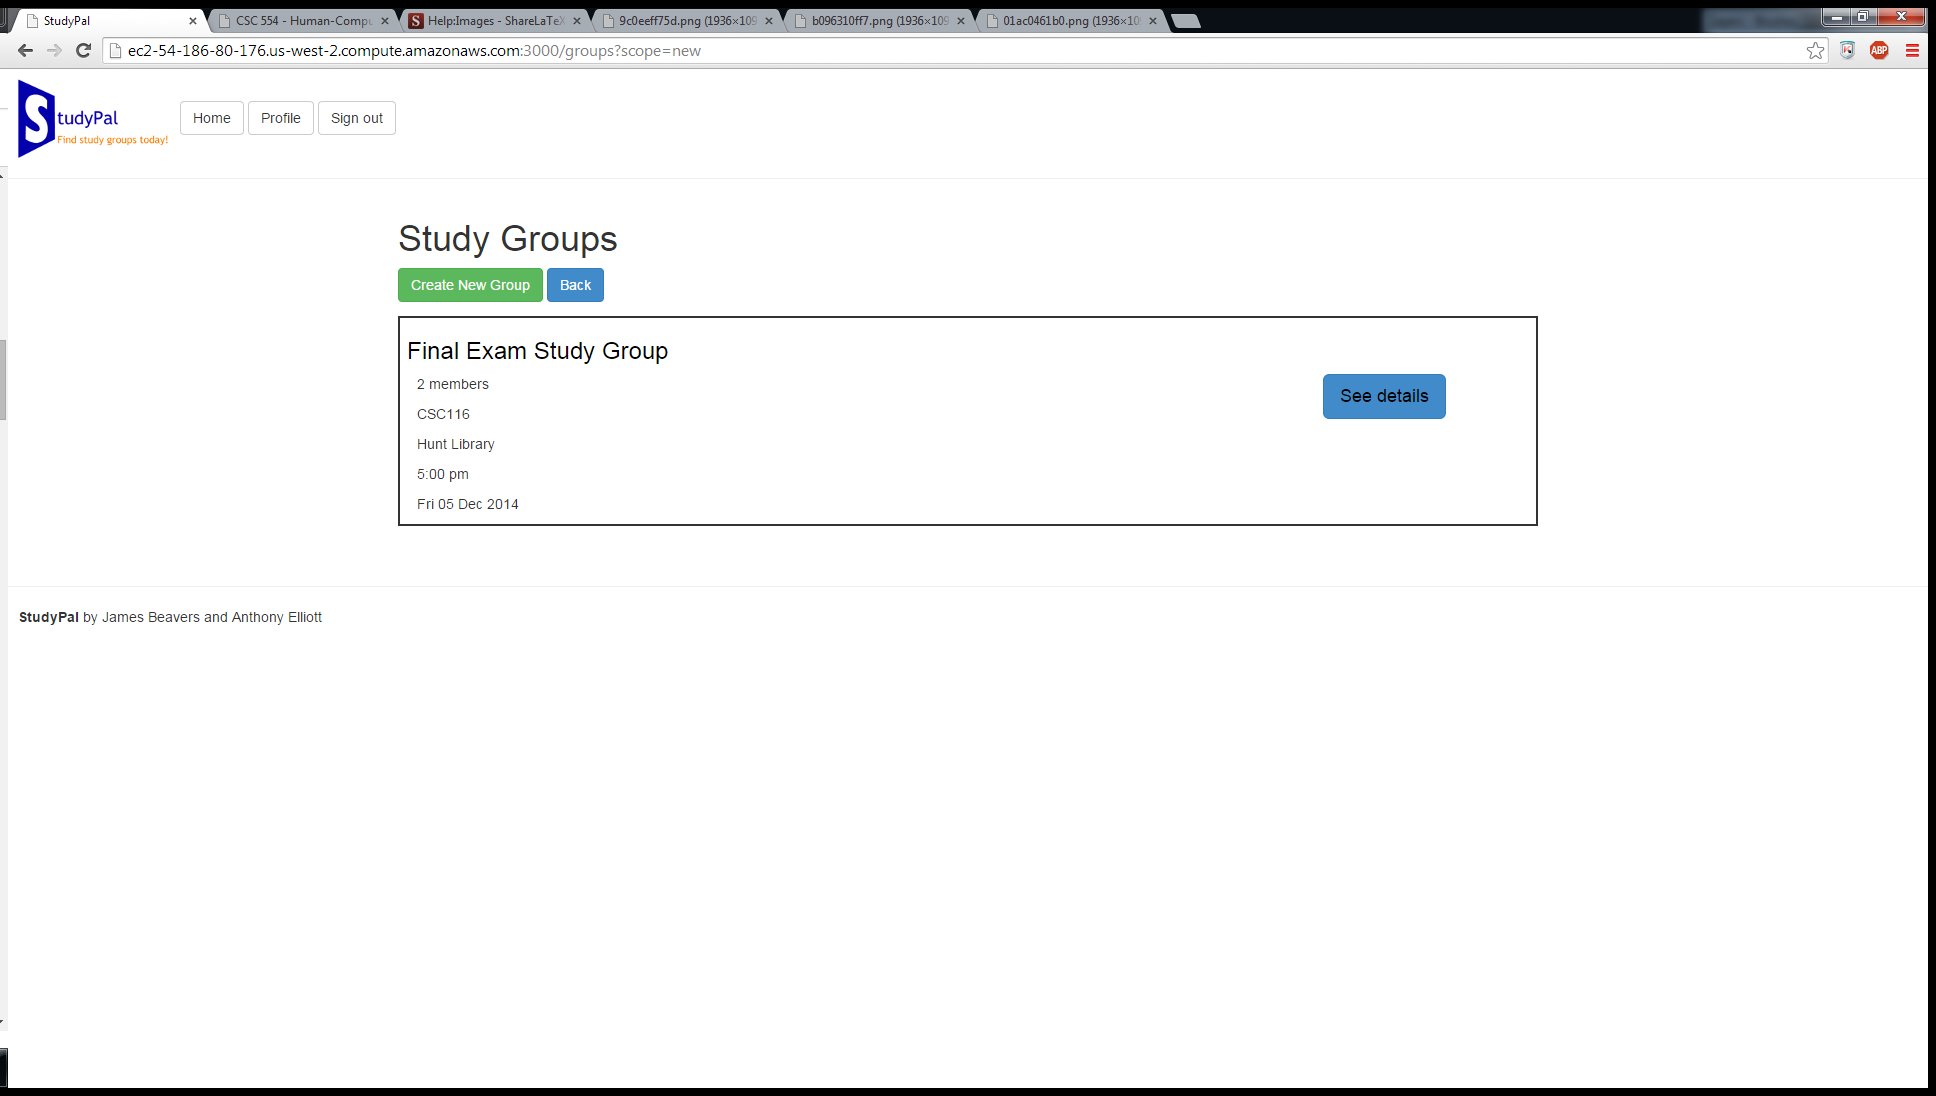
\includegraphics[width=80mm]{figures/groupList}
\caption{List of Study Groups \label{fig:groupList}}
\end{figure}

In the list, summary information about each group is displayed, such as course name and meeting date.  The user scrolls through the list of groups and selects one to view additional details.
The user looks at the desired qualifications of group members, as well as the existing group members' class schedules (figure~\ref{fig:groupDetails}).  The user will be able to see a Google Calendar displayed at the bottom of the group info page which has a combined view of all existing members' events (figure~\ref{fig:groupCalendar}).  If interested in joining, the user may select 'Apply'.  An application is submitted containing the applicant's name, email, and qualifications.
The group creator then sees (via a pending group applications list) that someone has requested group access and can choose to accept or reject this application (figure~\ref{fig:groupApplicationList}).

\begin{figure}[ht!]
\centering
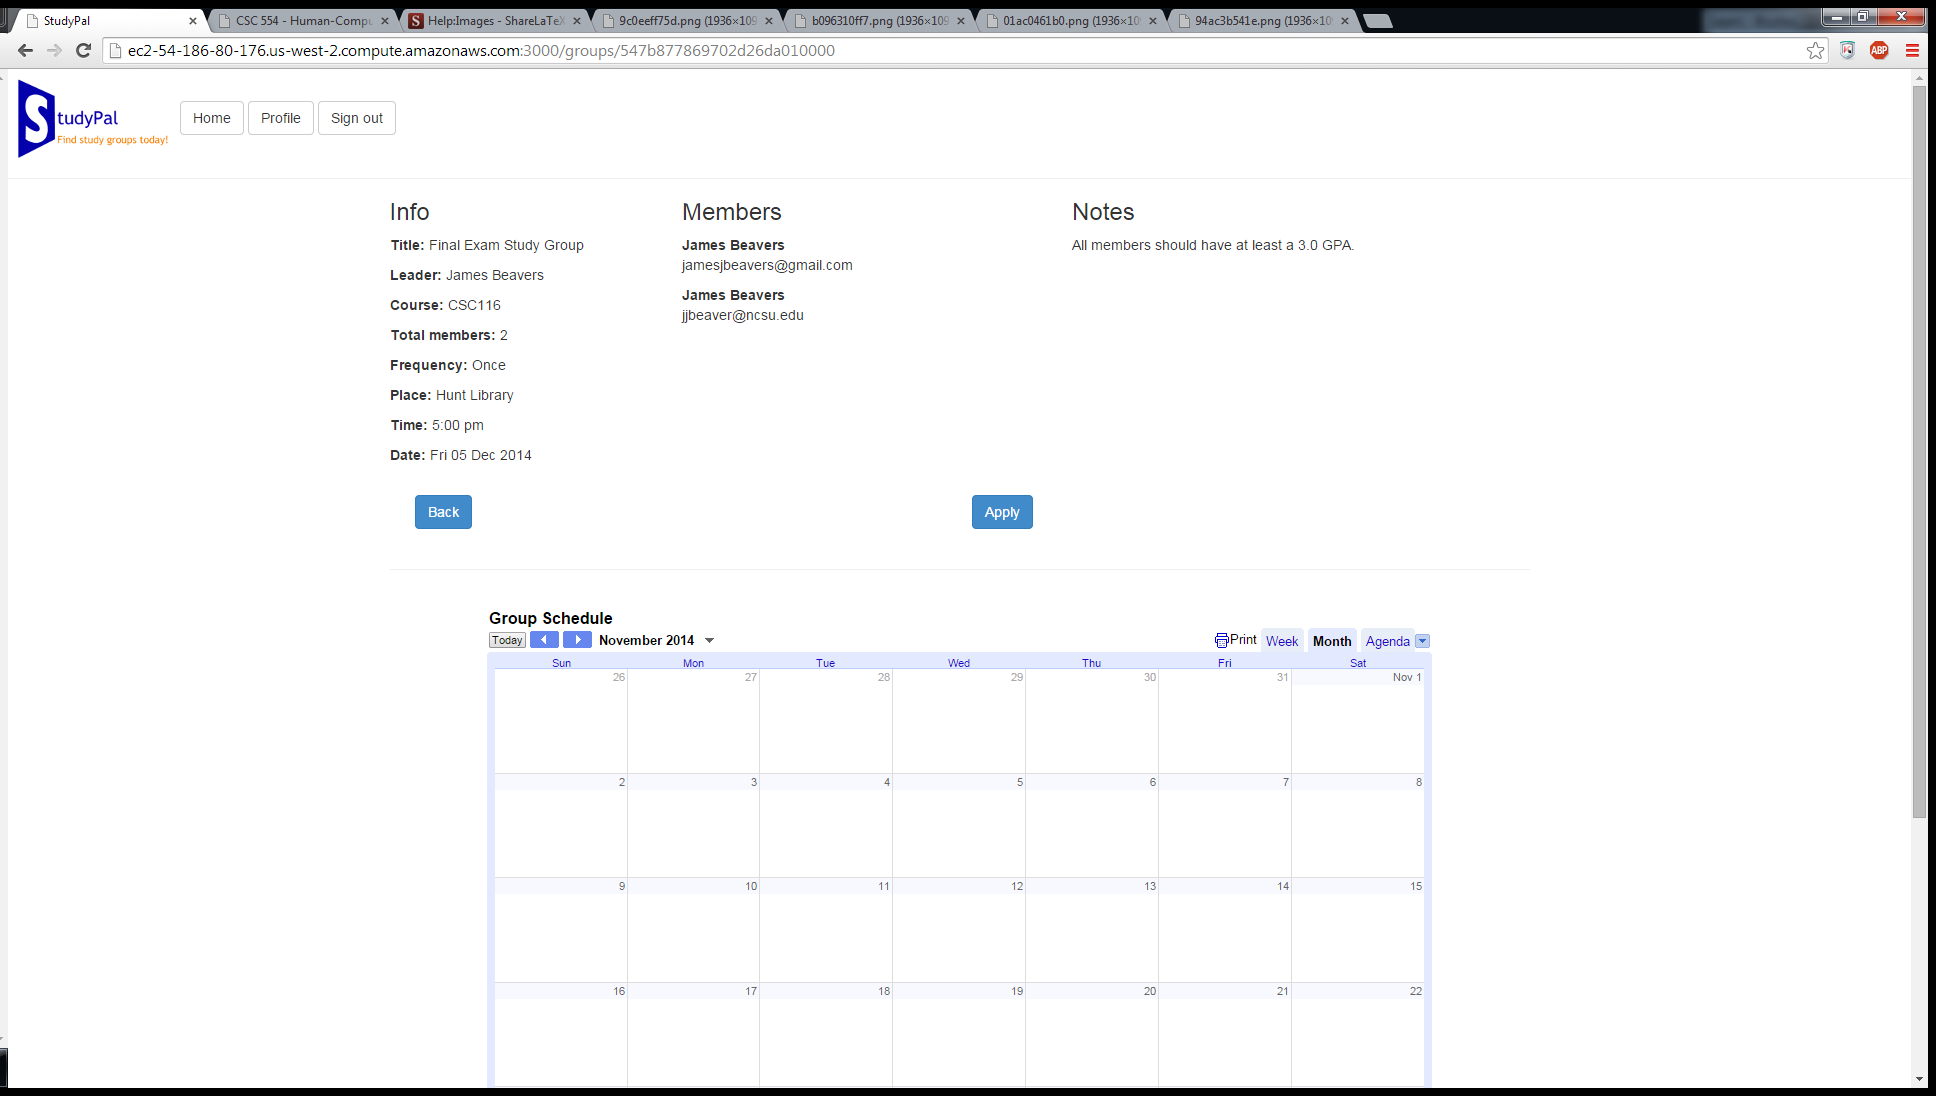
\includegraphics[width=80mm]{figures/groupDetails}
\caption{Group Details for Non-Member \label{fig:groupDetails}}
\end{figure}

\begin{figure}[ht!]
\centering
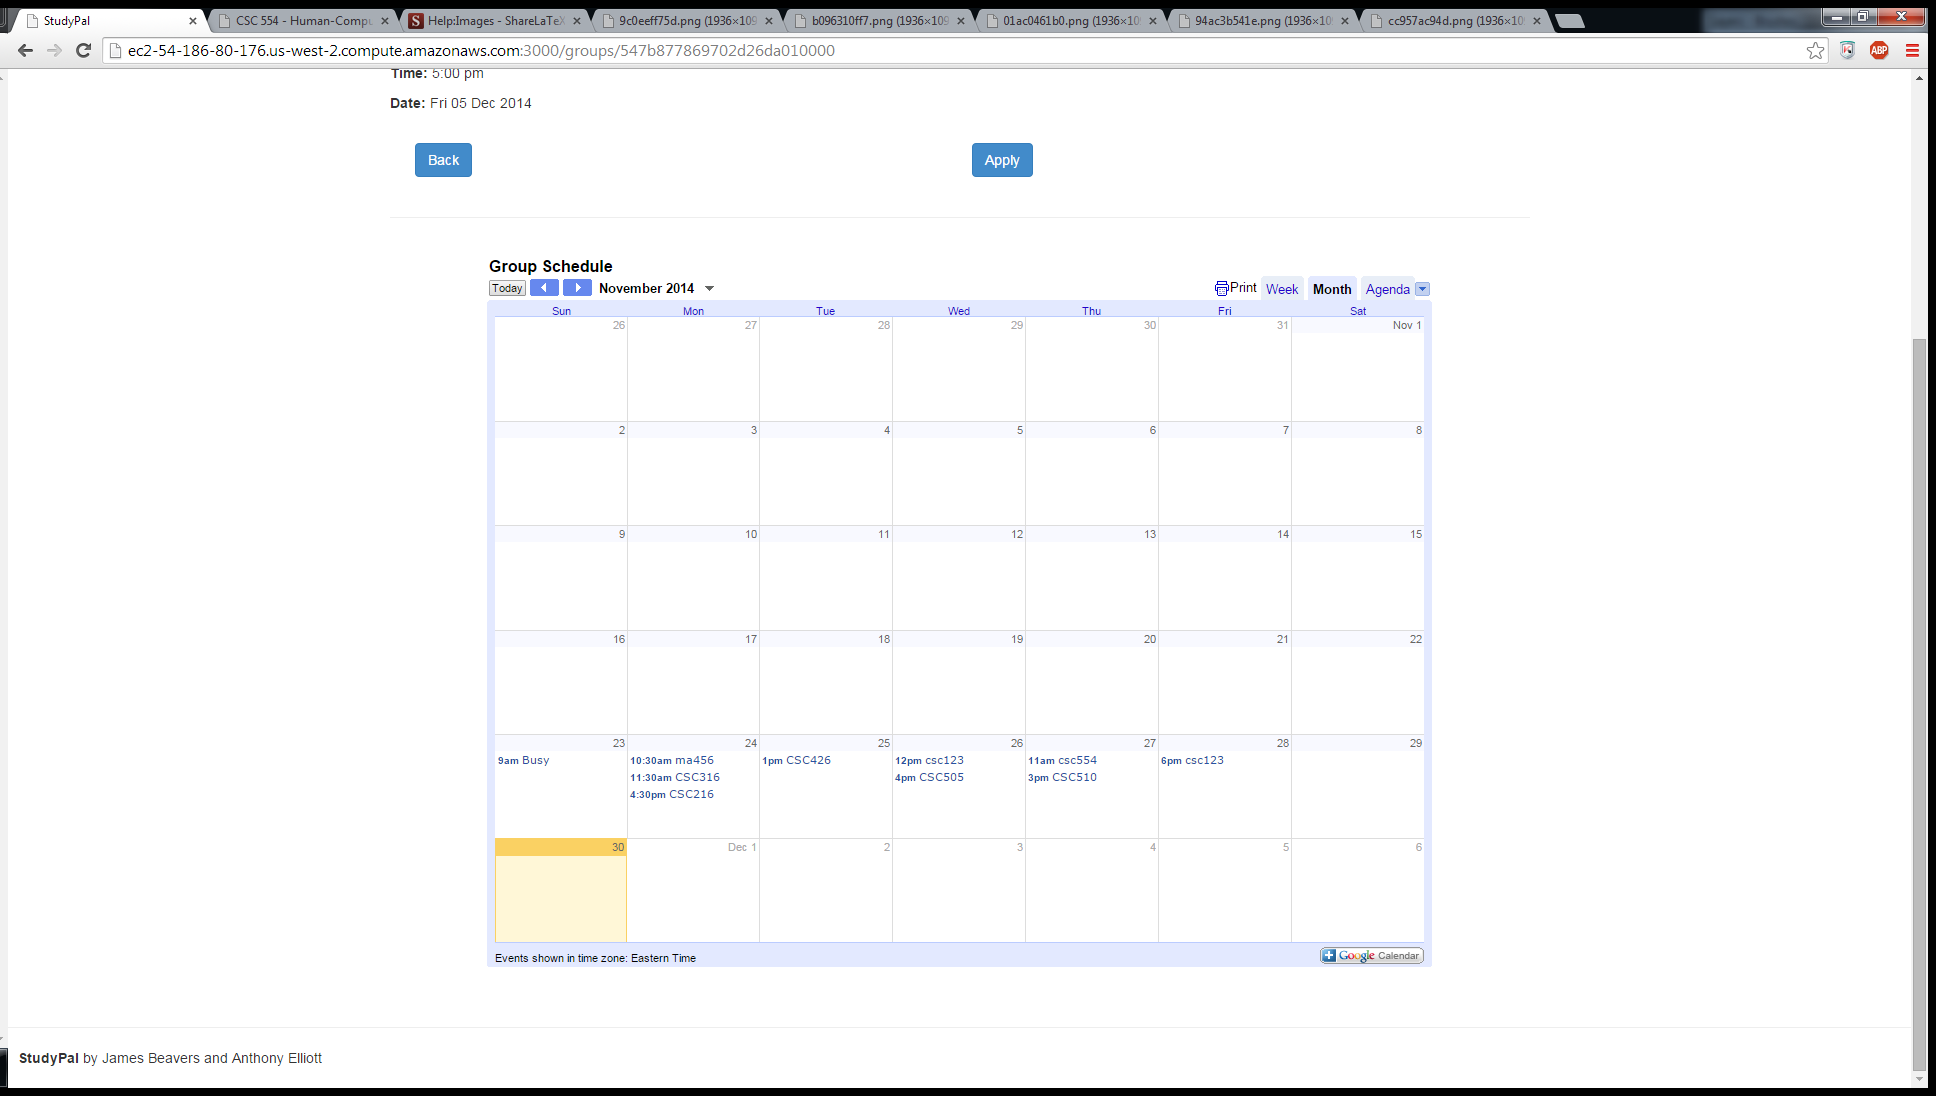
\includegraphics[width=80mm]{figures/groupCalendar}
\caption{Group Calendar \label{fig:groupCalendar}}
\end{figure}

\begin{figure}[ht!]
\centering
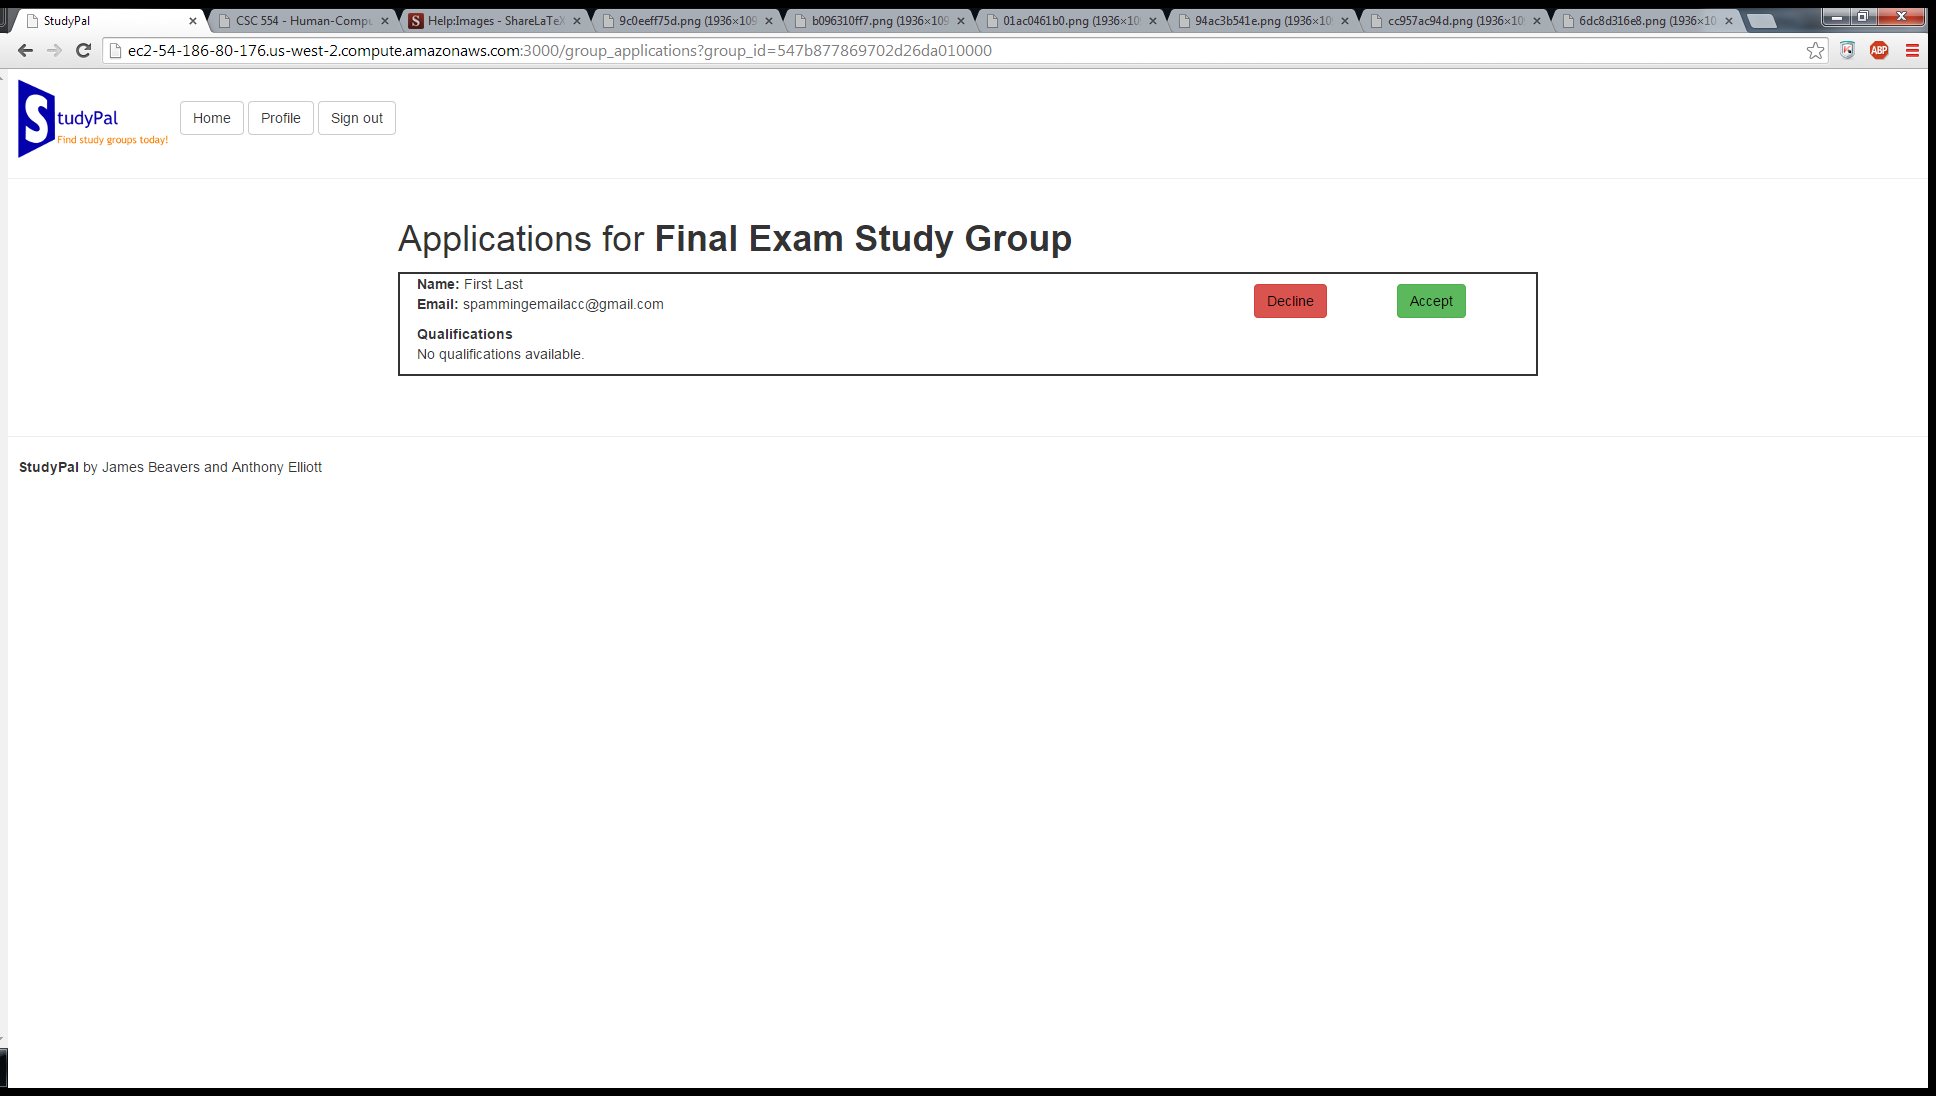
\includegraphics[width=80mm]{figures/groupApplicationList}
\caption{List of Group Applications \label{fig:groupApplicationList}}
\end{figure}

If there are no groups for the user's class or the user does not want to join any of the existing groups then they can create a group themselves.

\subsubsection{Leaving a Group}
A user who wishes to leave a study group first logs in to the StudyPal website, and selects 'My Groups' (figure~\ref{fig:home}).  From this list, the user can select the group which he or she is currently a member of and wishes to leave (figure ~\ref{fig:groupList}).  After selecting the group from the list, the user then selects the red 'Leave' button (figure~\ref{fig:groupDetailsMember}).  The user is prompted with a `Are you sure?' prompt for confirmation (figure~\ref{fig:confirmation}).  Once 'Ok' is selected, the user is removed the group.

\begin{figure}[ht!]
\centering
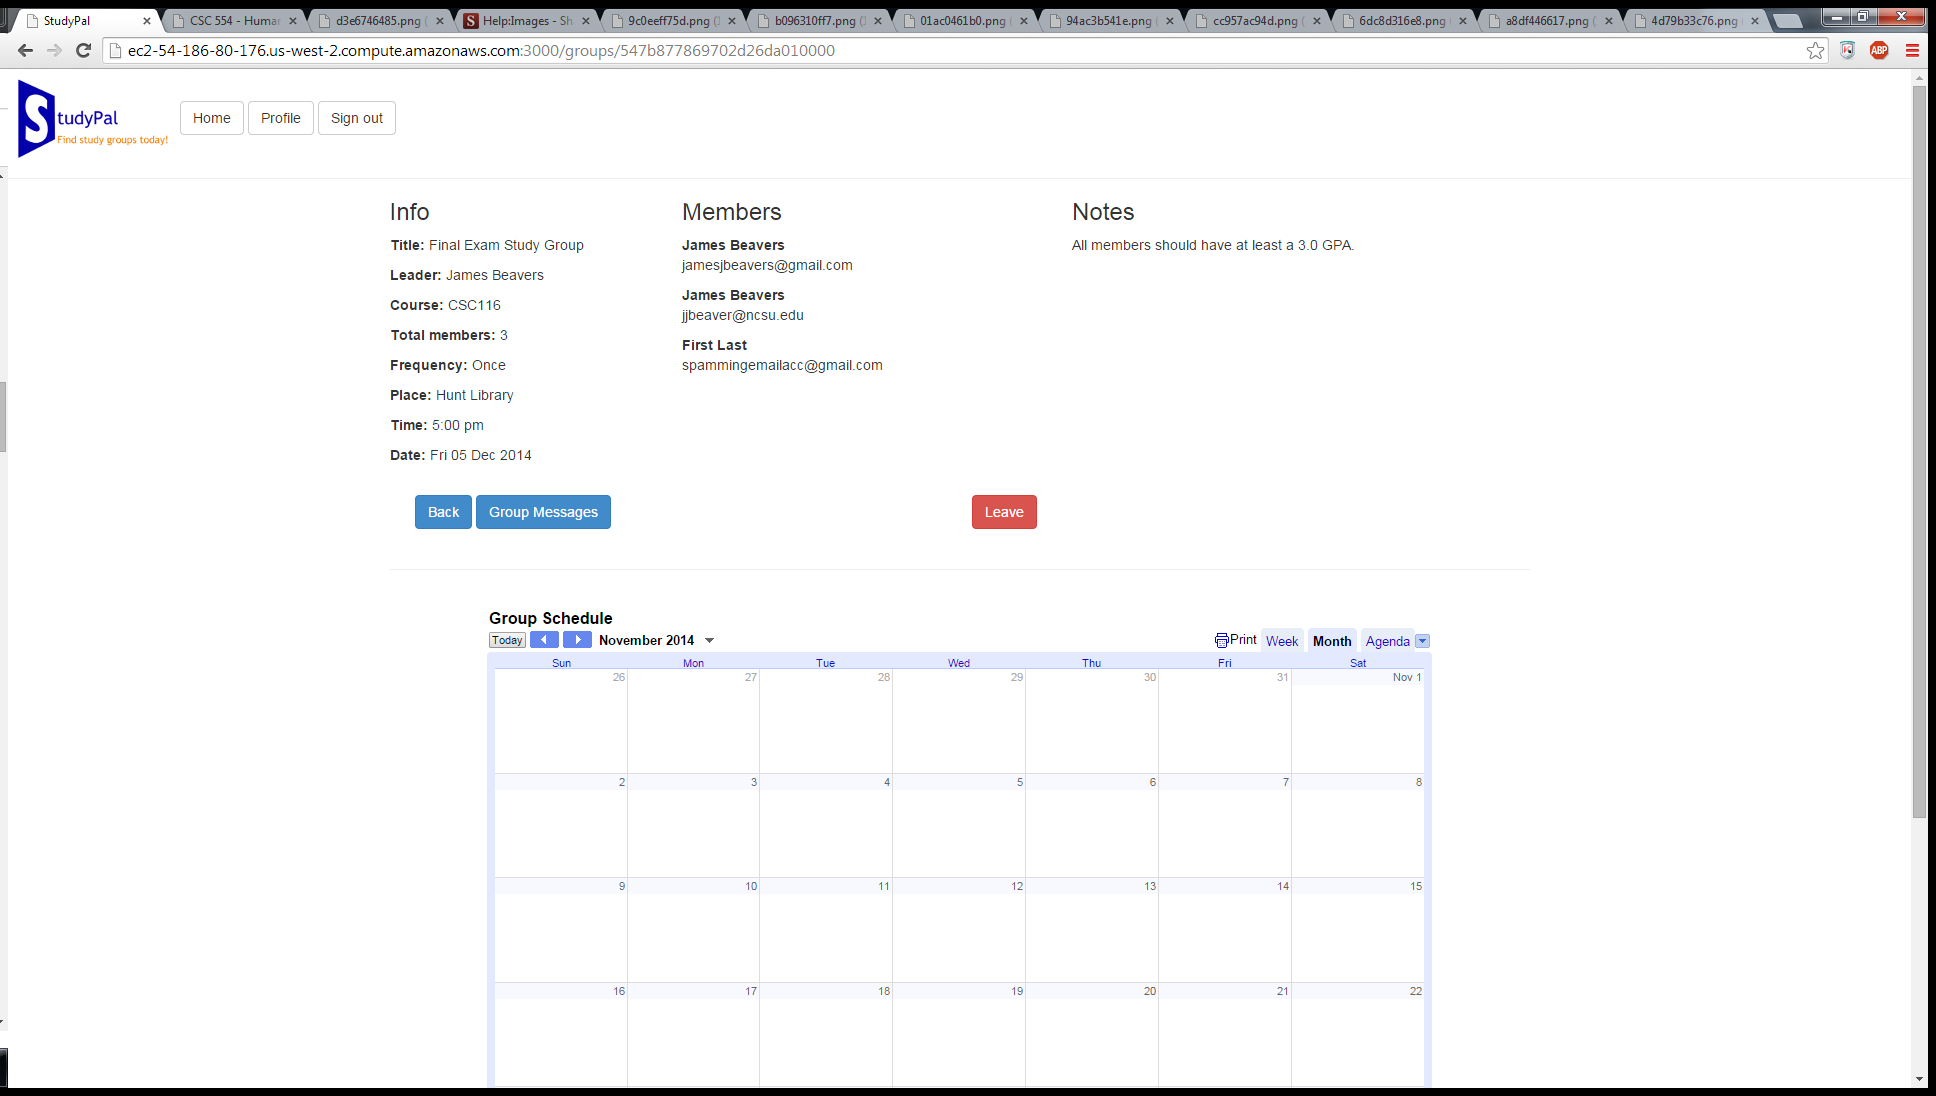
\includegraphics[width=80mm]{figures/groupDetailsMember}
\caption{Group Details for Member \label{fig:groupDetailsMember}}
\end{figure}

\begin{figure}[ht!]
\centering
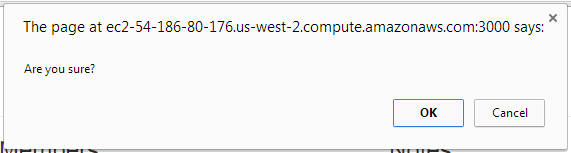
\includegraphics[width=80mm]{figures/confirmation}
\caption{Confirmation Message \label{fig:confirmation}}
\end{figure}

\subsubsection{Creating a Group}
A user who wants to create a study group first logs in to the StudyPal website, and hits the 'Create Group' button, which is displayed on the home page (figure~\ref{fig:home}), as well as a few other pages for convenience.
They enter basic information about the group, such as course and frequency of meetings (figure ~\ref{fig:newGroup}).
Fields such as time and place can be skipped if not yet decided on.
The user then enters qualifications such as 'have read all chapters', or 'attends all classes' that every group member should have.
This creates the group and the user waits for other students to see this group and apply to join. When students apply to the group, the applying student's qualifications are displayed in the application.
The user can then accept or reject these applications (figure~\ref{fig:groupApplicationList}).

\begin{figure}[ht!]
\centering
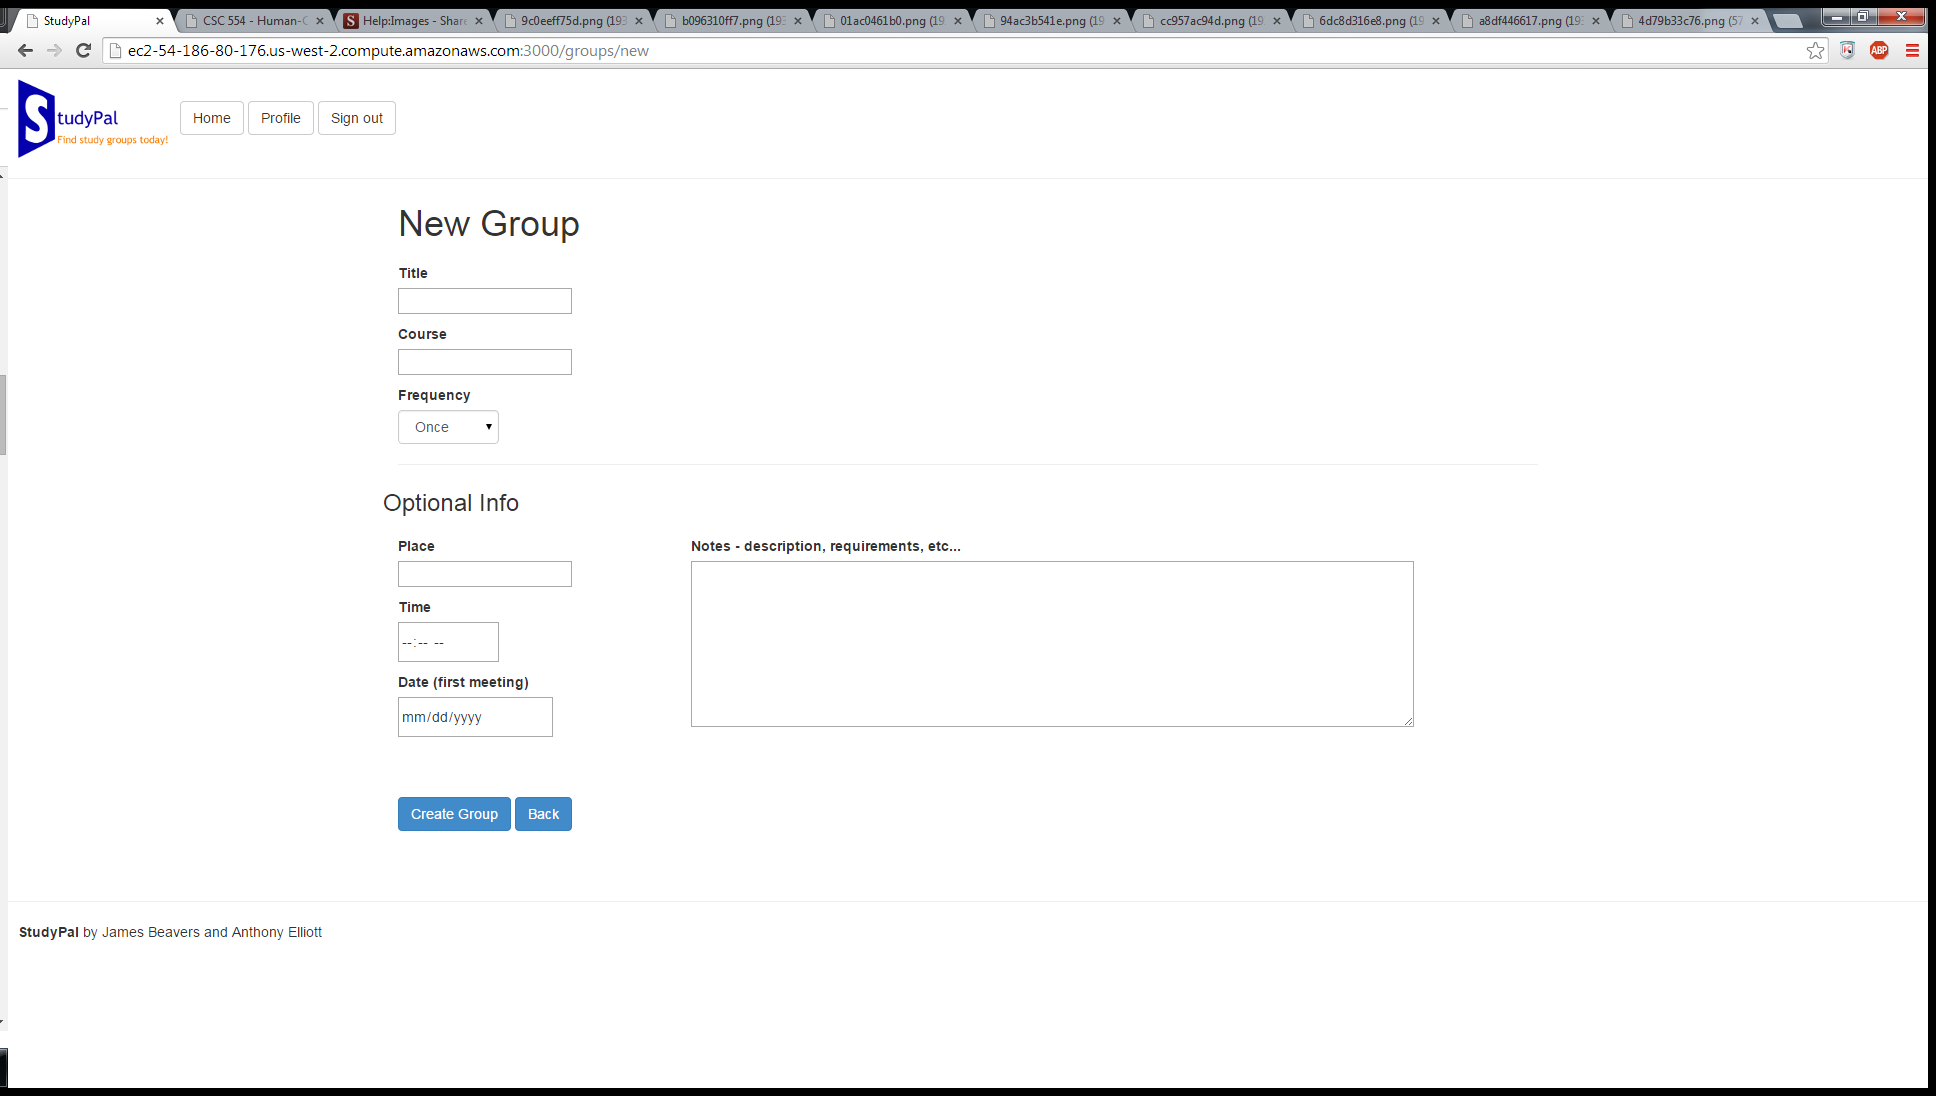
\includegraphics[width=80mm]{figures/newGroup}
\caption{New Group View \label{fig:newGroup}}
\end{figure}

\subsubsection{Deleting a Group}
A group leader who wishes to delete a group first logs in to the StudyPal website, and selects 'My Groups'.  From this list, the user can select the group (figure~\ref{fig:groupList}) which he or she is currently the leader and wishes to delete.  After selecting the group from the list, the user may select the red 'Destroy' button (figure~\ref{fig:groupDetailsLeader}).  The user will then be prompted with a confirmation message, 'Are you sure?' (figure~\ref{fig:confirmation}.  When the user selects 'Ok', the group is deleted, and the user is redirected to back to the home page.  All members and messages of the group are removed as well.

\begin{figure}[ht!]
\centering
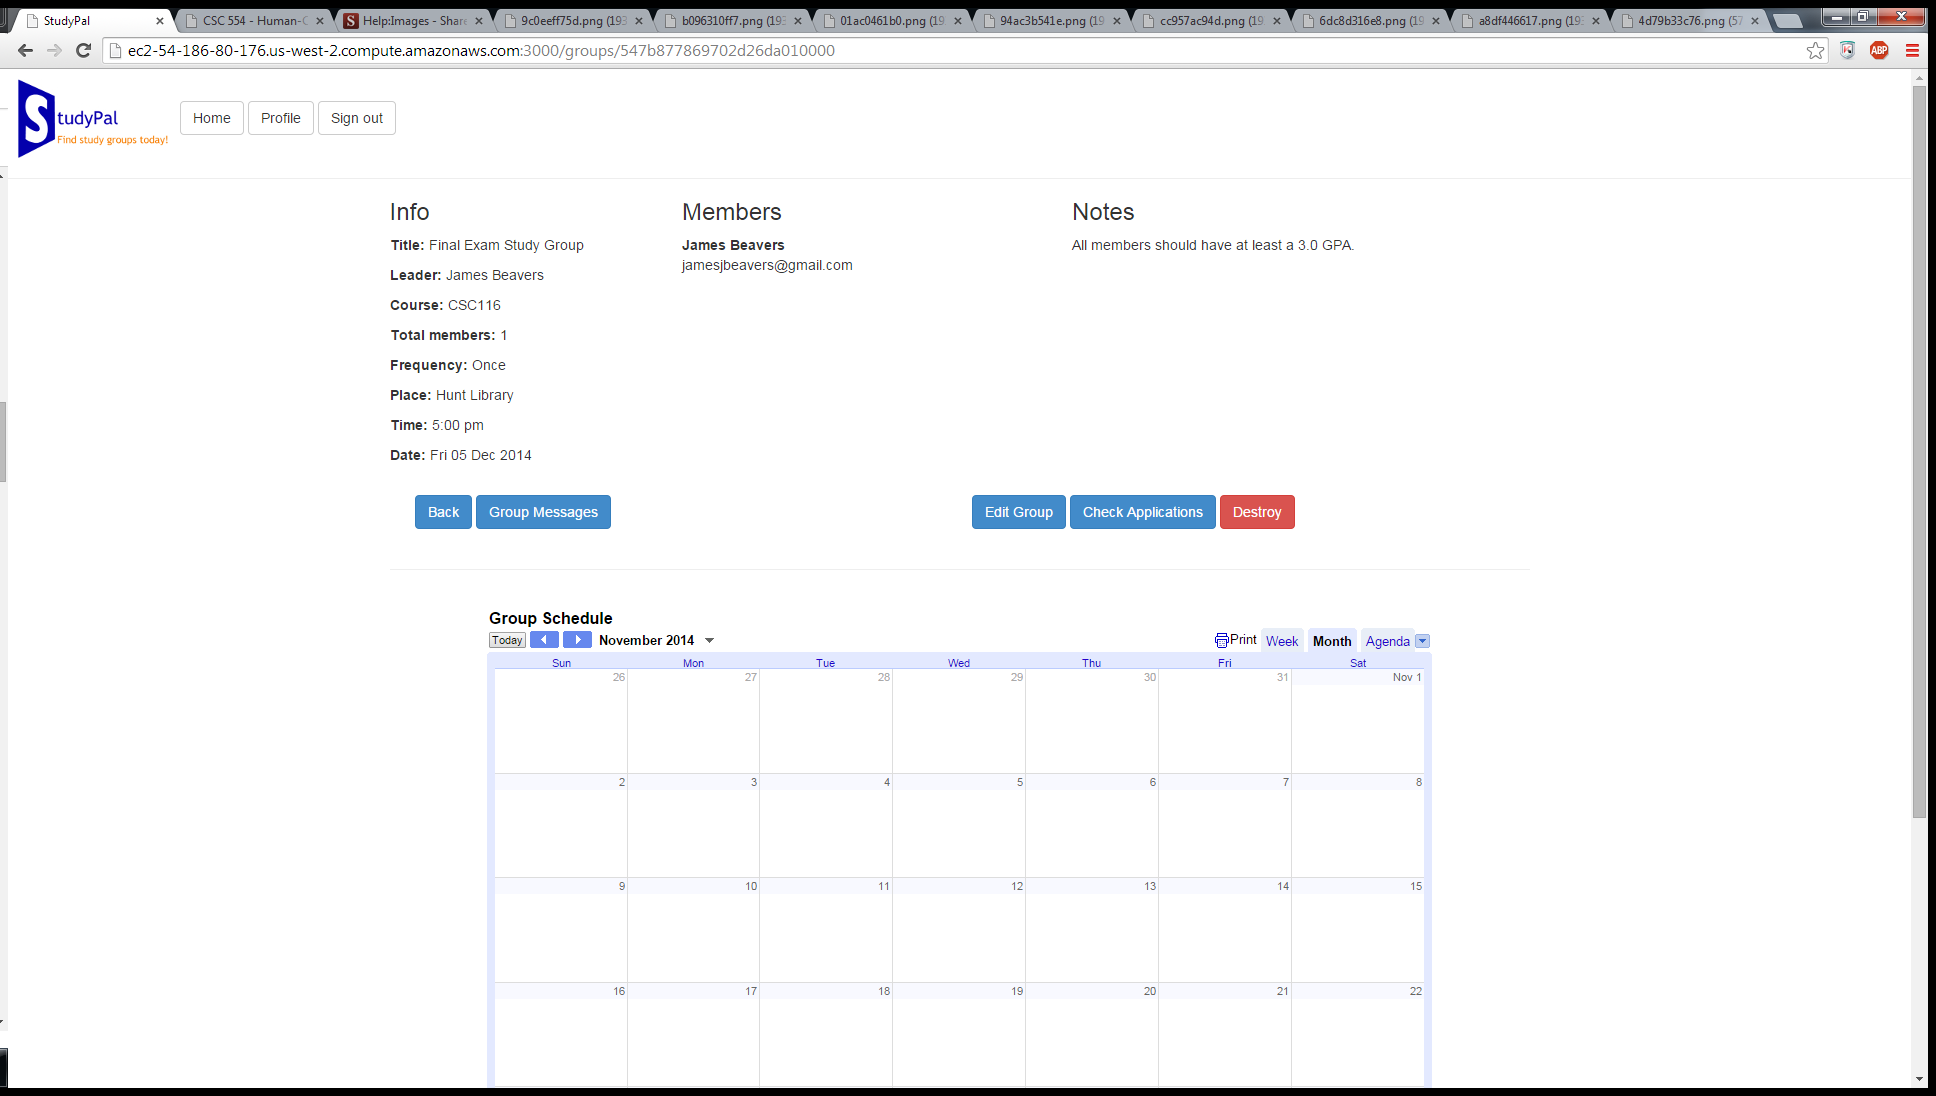
\includegraphics[width=80mm]{figures/groupDetailsLeader}
\caption{Group Details View for Leader \label{fig:groupDetailsLeader}}
\end{figure}

\subsubsection{Group Notifications}

Members of an existing group (users which either created the group or applied and were accepted) may wish to communicate with other group members.  A group member/leader may view his or her groups via the "My Groups" button on the home page.  The user then selects one of the groups from the list.  In the group view, the user then selects "Check Messages" (figure~\ref{fig:groupDetailsMember}).  A list of that particular group's messages is displayed (figure~\ref{fig:messageList}).  Each message has the sender (one of the group members), the sender's email, a timestamp for when the message was posted, and a message body.  At the top of this page is a button "New Message" to create a new message.  When selected, the user may enter a message up to six hundred characters in length.  The user then selects "submit" and the message is added to the list (figure~\ref{fig:newMessage}).  

\begin{figure}[ht!]
\centering
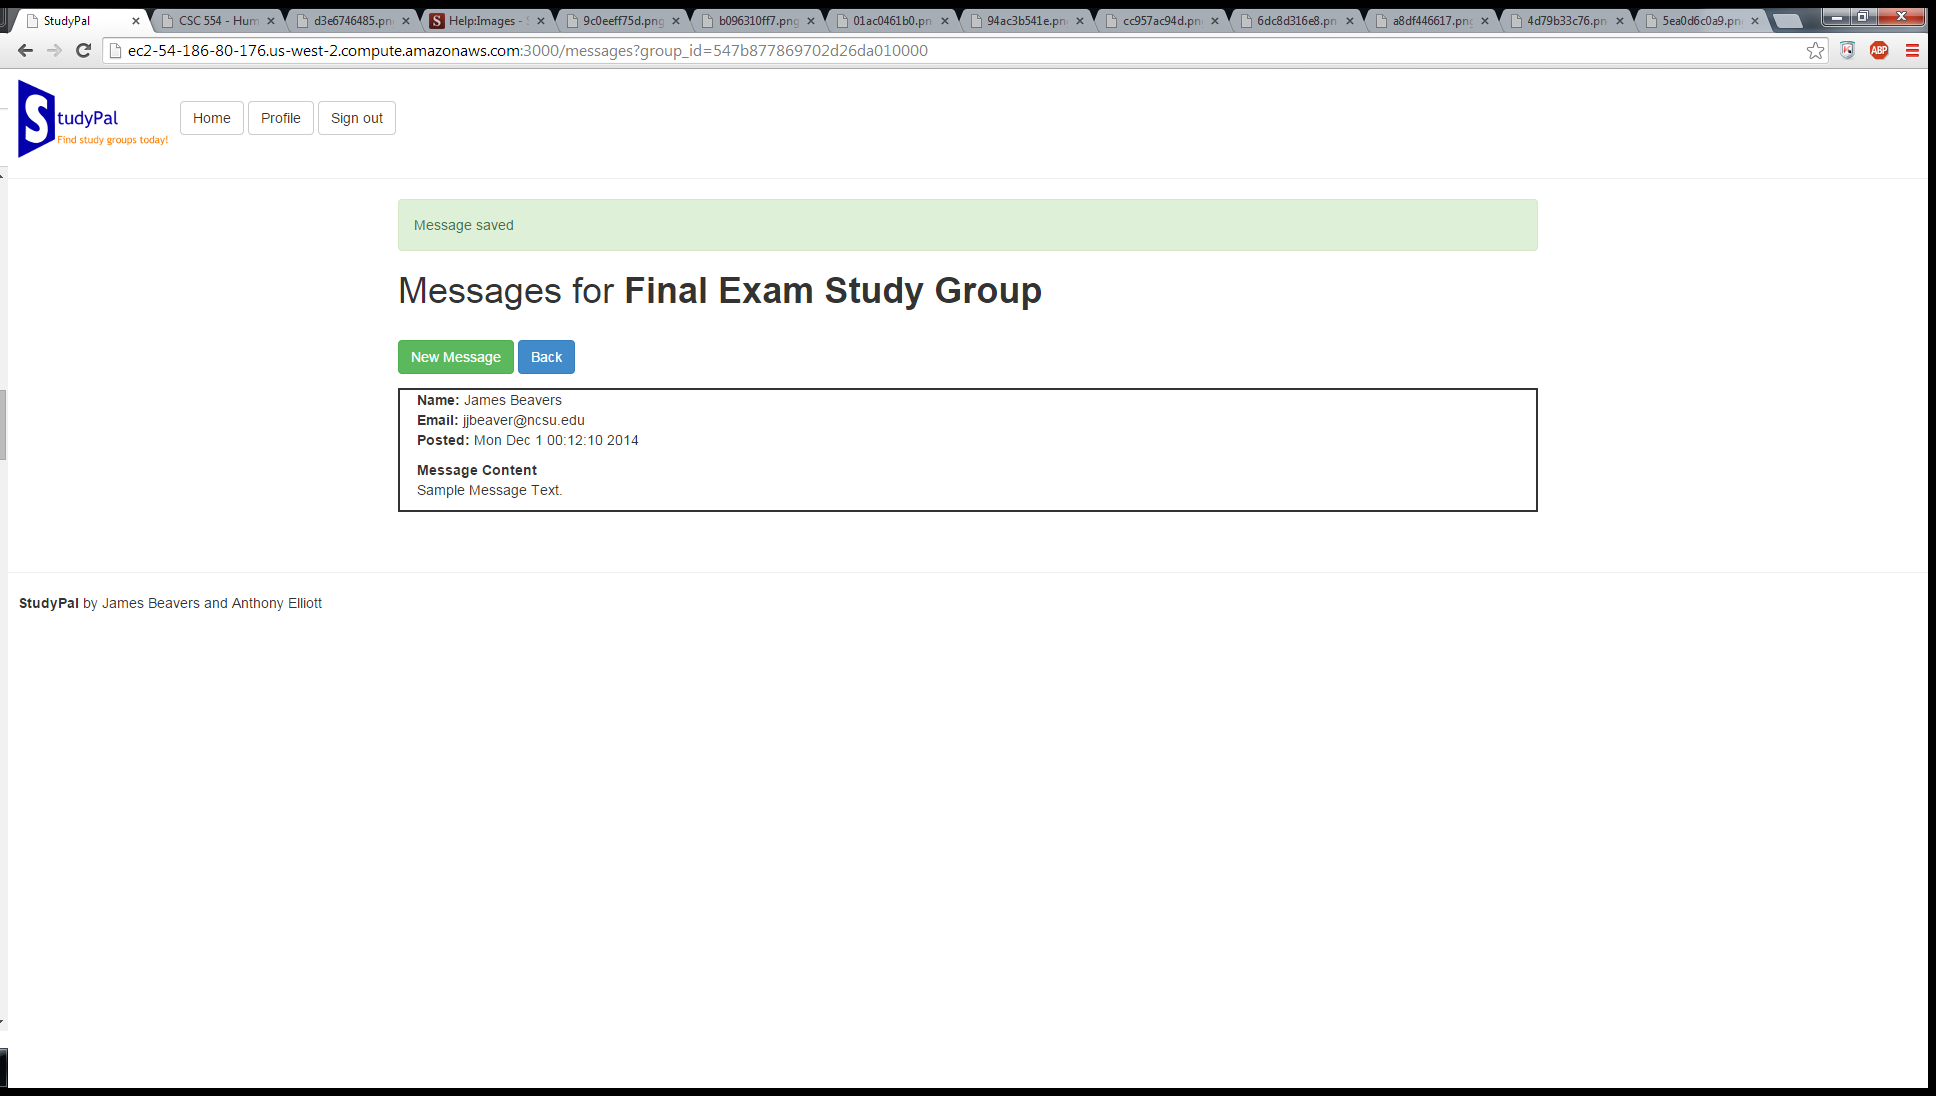
\includegraphics[width=80mm]{figures/messageList}
\caption{List of Group Messages \label{fig:messageList}}
\end{figure}

\begin{figure}[ht!]
\centering
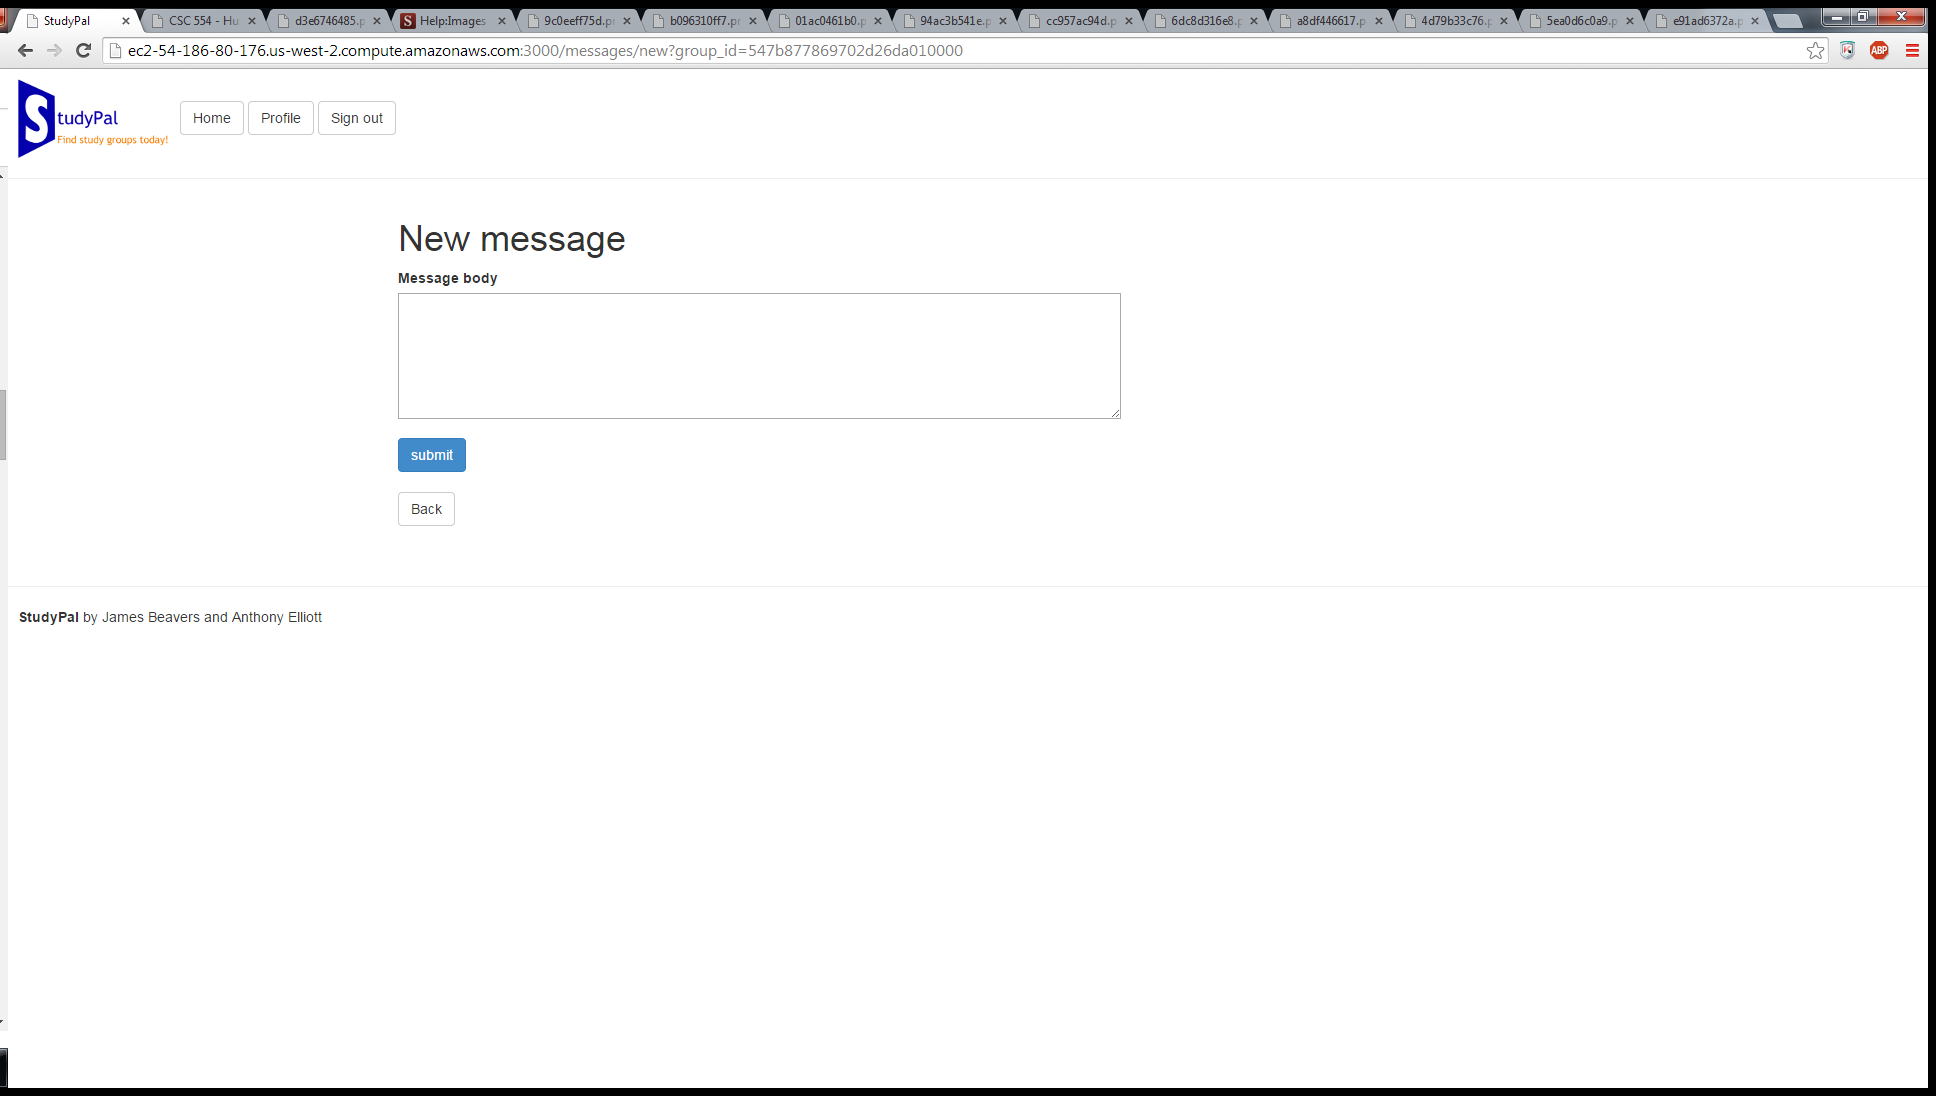
\includegraphics[width=80mm]{figures/newMessage}
\caption{New Message View \label{fig:newMessage}}
\end{figure}

Additionally, the names and email addresses of all members of a group is displayed on the group info page so that members may choose to contact each other via email as well.

\section{Related Work and Influences}

StudyPal was influenced by a number of systems and readings.  Firstly, user login was heavily influenced by the trend to allow sign on with social media accounts.  Because of this, along with the convenience of using Google Calendars to handle class scheduling, we decided to allow sign on with Google accounts.  Other popular group forming websites such as \emph{www.meetup.com} allow signing on with a social media account - Facebook in this case.

In choosing our color scheme for StudyPal, we tried to adhere to basic color theory principles\cite{thomas:color:online}.  In particular, we tried to present text with a color that strongly contrasted its background.  We also tried to use colors which complemented each other.  This was especially crucial when designing a logo and the accompanying buttons colors that appears throughout our application.

\section{System Design}


% user interviews
% sketches
% development
% user feedback (where I'm the user)

We wanted to create a very simple user interface that could be quickly used by an expert.
We also wanted our website to be easy to use for novices, that is, we wanted novices to be able to complete basic tasks in the website without requiring outside help.
The specific tasks that we wanted to support are joining an existing group, creating a new group, and sending notifications to the group members.

We first started by interviewing several students who have previously used study groups for their classes in order to better determine the scope of our system.

After extracting requirements from the interviews, we sketched mockups of the website using pencil and paper.
%todo These sketches are included in ____
The sketches helped us identify challenges that we would face.

One challenge was how to integrate the user's schedule into our system.
One user said that ``even though courses appear on my schedule, I don't always have to go to them and would still be available to meet.''
This highlights the issue that a schedule may not be accurate for all users and thus we don't want to hide groups that meet during these times in case the user actually wants to attend those meetings.
As a compromise, we decided to show all groups, with some summary information about each group in the list view.  If the summary information seems acceptable to the user, the user can navigate to the detailed group view to see the combined Google Calendar class schedule of all group members.  The user can then visually inspect this calendar to see if it meets their preferences for availability.



In interviews, one participant said that ``the level of distraction increases with the number of people in the group.''
The same participant said that 5 study group members was the upper limit for productivity, however, other interview participants said they frequently had study groups with around 5 members.
This shows that a generally small group is more desirable, but further research is needed to see how group size impacts study group results.
We decided to prominently display the current group size for potential applicants so that they could make their own decision if they wanted to join a group with 5 or more members.

Another issue was group member requirements.
We discovered in interviews that study groups are usually formed via personal connections and many subjective decisions were made to determine who to invite to the group.
One participant said that all study group members ``need a common background'', for example, each member should have at least passing familiarity with each section of material.
Defining this 'common background' is an example of such subjective decisions.
We did not want to implement complex qualification algorithms without basing decisions on solid research, so we allow group leaders to create subjective qualifications and decide themselves.
Group leaders enter desired qualifications of group members, other students can apply after reading through the qualifications, and then the leader reviews each application and can either accept or reject them.


Frequency of study groups is another issue that emerged from the interviews.
Some students typically formed a study group that only met once per exam while others met on a regular basis.
We extracted discrete intervals of once, weekly, monthly, and other for study groups.


To see the sketched which resulted from these interviews and feedback, see Appendix A.



\section{Analytical Interface Evaluation}
%An analytical evaluation of your interface, using modeling techniques you judge to be most appropriate. 
 
%\emph{A specific analytical technique modeling technique is correctly applied; its choice is well-justified and the results are explained in detail. The analytical technique is such that it provides predictions or explanations of actual user performance. Insights from the analytical evaluation are discussed. The relevance of the modeling results to usability are made clear.}

% use the KLM
 
In this section we provide an analytical evaluation of StudyPal.
Specifically, we describe why we chose the KLM model\cite{Card:KLM}, how we applied the model to three use cases of StudyPal, and what these results mean in terms of the usability of StudyPal.

\subsection{Relevance to Usability - Why KLM?}
The Keystroke-Level Model (KLM) \cite{Card:KLM} is a simple model to predict how long expert users will need to perform a given task on a computer system.
Limiting the scope of our analysis to `expert' users who rarely make mistakes makes sense for initial predictions.
As more people use StudyPal, exploring alternative methods could add more value with more accurate predictions.

One such alternative is ACT-R\cite{Anderson:ACT-R} which offers more accurate predictions, but takes much more effort.
Another alternative is NGOMSL\cite{Kieras:NGOMSL} which incorporates learning in order to extend the scope of the predictions

In this context, an `expert' user is simply one that is accustomed to using academic tools which involve groups, classes, messaging, etc.  Examples of these types of tools include Moodle and WolfWare.

With these predictions, we will be able compare with actual results of real users carrying out these tasks.  With this comparison, we can see where the largest differences lie and where we may have missed potential usability concerns - e.g. patterns that can be eliminate so that the total number of user actions is minimized.

% explain why using the KLM
 % sufficient for our needs
 % a more detailed analysis would benefit from the NGOMSL because it factors in learning time
 % KLM limitations: 
   % errors
   % learning
   % functionality
   % recall
   % concentration
   % fatigue
   % acceptability
 % we don't care much about the missing pieces above (except learning)

\subsection{Application of KLM}
We describe how we applied the KLM to the three main use cases of StudyPal.
All five use cases, or tasks, assume that the user is already logged in to StudyPal and located at the home page.

\subsubsection{Joining a Group}
The user must first click on the ``Explore Groups'' button, then click on a group to display group details, read the displayed information and then hit 'Apply'.

\paragraph{List all groups:}
This requires the user to home (H) their hand to the mouse, point (P) at the button with the mouse, and click (K) the button using the left mouse button.
The user then waits for StudyPal to respond (R).

In the KLM, this is encoded as: \emph{HPKR}.

The KLM predicts that homing takes 0.4 seconds, pointing takes 1.1 seconds, and the key press takes 0.2 seconds.
This results in a time of 1.7 seconds to list all existing groups, assuming negligible system response time.

\paragraph{Display group details:}
Now that the system has displayed all existing groups, the user must find one they are interested in joining.
The user should already have their hand on the mouse from the previous action, so we will not factor a homing action in here.
This task requires the user to point (P) with their mouse to the name of the group they want to join, click (K), and then wait for the system to respond (R).

In the KLM, this is encoded as: \emph{PKR}.

The KLM predicts the pointing to take 1.1 seconds, the button press to take 0.2 seconds, and the system response time is assumed to be negligible.
This results in a time of 1.3 seconds to display the details of a group.

\paragraph{Apply:}
Once displayed with the group details, the user needs to hit the 'Apply' button to submit their application to the group leader.
The user should already have their hand on the mouse from the previous action, so we will not factor a homing action in here.
This task requires the user to point (P) with their mouse to the 'Apply' button, click (K), and then wait for the system to respond (R).

In the KLM, this is encoded as: \emph{PKR}.

The KLM predicts the pointing to take 1.1 seconds, the button press to take 0.2 seconds, and the system response time is assumed to be negligible.
This results in a time of 1.3 seconds to apply to a group.

The user must now wait for the study group leader to review their application before being allowed formal entrance into the group.

\textbf{Total time:}
Combining the above encodings we get \emph{HPKRPKRPKR} in the KLM and a total time of 4.3 seconds to apply to a group.

\subsubsection{Leaving a Group}
The user must first click on the ``My Groups'' button, then click on a group they wish to leave.  The group details page loads and then the user will click ``Leave''.  A confirmation message will appears and the user will click ``Ok''.

\paragraph{List `my' groups:}
This requires the user to home (H) their hand to the mouse, point (P) at the button with the mouse, and click (K) the button using the left mouse button.
The user then waits for StudyPal to respond (R).

In the KLM, this is encoded as: \emph{HPKR}.

The KLM predicts that homing takes 0.4 seconds, pointing takes 1.1 seconds, and the key press takes 0.2 seconds.
This results in a time of 1.7 seconds to list all existing groups, assuming negligible system response time.

\paragraph{Display group details:}
Now that the system has displayed all existing groups that the user is a member of, the user must find one they are interested in leaving.
The user should already have their hand on the mouse from the previous action, so we will not factor a homing action in here.
This task requires the user to point (P) with their mouse to the name of the group they want to leave, click (K), and then wait for the system to respond (R).

In the KLM, this is encoded as: \emph{PKR}.

The KLM predicts the pointing to take 1.1 seconds, the button press to take 0.2 seconds, and the system response time is assumed to be negligible.
This results in a time of 1.3 seconds to display the details of a group.

\paragraph{Leave:}
Once displayed with the group details, the user needs to hit the 'Leave' button. The user will then be prompted with a confirmation message.  The user will need to click 'Ok' to leave the group. The user should already have their hand on the mouse from the previous action, so we will not factor a homing action in here.
This task requires the user to point (P) with their mouse to the 'Leave' button, click (K), and then wait for the system to respond (R). Then, the user will point (P) to the 'OK' button, click (K), and then wait for the system to respond (R) again.

In the KLM, this is encoded as: \emph{PKRPKR}.

The KLM predicts the pointing to take 1.1 seconds, the button press to take 0.2 seconds, and the system response time is assumed to be negligible.
This results in a time of 2.6 seconds to leave the group (at the group detail screen).


\textbf{Total time:}
Combining the above encodings we get \emph{HPKRPKRPKRPKR} in the KLM and a total time of 5.6 seconds to leave a group.


\subsubsection{Creating a Group}
The user must first click on the ``Create group'' button, enter the group title, enter the course name, select the frequency of meeting, and then submit the form.
Other optional information fields exist but we exclude them from this model as they are not part of the minimum action set needed to create a group.

\paragraph{Click ``Create group'':}
From the home page, the user needs to click the `Create group' button.
This requires the user to home (H) their hand to the mouse, point (P) at the button with the mouse, and click (K) the button using the left mouse button.
The user then waits for StudyPal to respond (R).

In the KLM, this is encoded as: \emph{HPKR}.

The KLM predicts that homing takes 0.4 seconds, pointing takes 1.1 seconds, and the key press takes 0.2 seconds.
This results in a time of 1.7 seconds to display the form for group creation, assuming negligible system response time.

\paragraph{Enter group title:}
After the group creation form has been displayed, the user must enter a title for this group.
For the purposes of this model we will assume that the average group name consists of two words, and that each word consists of an average length of five characters\footnote{http://www.wolframalpha.com/input/?i=average+word+length}.
In totaling the characters, we find that there are 10 characters plus one delimiter such as a space or dash resulting in an average group title length of 11 characters.

To enter this, the user must first point (P) with the mouse to the input field, click (K) to select the input field, home (H) their hands to the keyboard, enter one word of 5 characters, enter a space, and enter another word of 5 characters.
We have spaced the following encoding to represent these actions.

This results in a KLM encoding of \emph{PKH MKKKKK K MKKKKK}.
The KLM predicts that pointing will take 1.1 seconds, each of the 12 key presses will take 0.2 seconds, the homing will take 0.4 seconds, and the single act of mental preparation will take 1.35 seconds.
This results in a total time of 4.89 seconds to enter the title of the group.

\paragraph{Enter course name:}
After entering the group title, the user must enter the name of the course this group will be studying.
Most university courses can be represented with a three letter department indicator (e.g. CSC for Computer Science) and a three digit course number (e.g. 554).

To enter this, the user can home (H) to the keyboard, hit the TAB button (K) to move to from the title input form to the course name input form, type the three letter department abbreviation (KKK), type a space (K), and finally type the three digit course number (KKK).

Combining these encodings with needed mental preparation results in a KLM encoding of \emph{HKMKKKKMKKK}.
The KLM predicts that the homing act will take 0.4 seconds, each of the 8 key presses will take 0.2 seconds, and the mental preparation will take 1.35 seconds.
This results in a total time of 3.35 seconds to enter the course name.

\paragraph{Select frequency:}
After entering the course name, the user must select one of three frequencies (meet once, meet weekly, or meet monthly) from a drop down menu.
We select `Once' by default as we expect this to be the most common of the three.
If the user wants to keep the default frequency of `Once' then this entire step can be skipped.

Otherwise, the user will need to home (H) their hands to the keyboard, hit the TAB button (K) to select the frequency drop down menu, and hit the down arrow key twice (KK) to advance from `Once' to `Weekly' to `Monthly'.

This results in a KLM encoding of \emph{HKMKK}.
The KLM predicts that the homing act will take 0.4 seconds, each of the 3 key presses will take 0.2 seconds, and the mental preparation will take 1.35 seconds.
Thus frequency selection is predicted to take a total time of 2.35 seconds.

\paragraph{Submit form:}
After entering all required information, the user must submit the form by hitting the ENTER button.

The user must home (H) to the keyboard, hit the ENTER key (K), and wait for the system to respond (R).
This results in a KLM encoding of \emph{HKR}.
The KLM predicts that the homing will take 0.4 seconds, the single keypress will take 0.2 seconds, and we assume a negligible system response time.
Thus we predict form submission to take 0.6 seconds.

\textbf{Total time:}
Here we sum the time of each subtask.
Clicking `Create group' is predicted to take 1.7 seconds,
entering the group title should take 4.89 seconds,
entering the course name should take 3.35 seconds,
selecting the frequency should take 2.35 seconds,
and form submission should take 0.6 seconds.

This results in a total time of 12.89 seconds to create a group.


\subsubsection{Deleting a Group}
The user must first click on the ``My Groups'' button, then click on a group they wish to delete.  The group details page loads and then the user will click ``Destroy''.  A confirmation message will appears and the user will click ``Ok''.

\paragraph{List `my' groups:}
This requires the user to home (H) their hand to the mouse, point (P) at the button with the mouse, and click (K) the button using the left mouse button.
The user then waits for StudyPal to respond (R).

In the KLM, this is encoded as: \emph{HPKR}.

The KLM predicts that homing takes 0.4 seconds, pointing takes 1.1 seconds, and the key press takes 0.2 seconds.
This results in a time of 1.7 seconds to list all existing groups ("my groups"), assuming negligible system response time.

\paragraph{Display group details:}
Now that the system has displayed all existing groups that the user is a member of, the user must find one they are interested in deleting.
The user should already have their hand on the mouse from the previous action, so we will not factor a homing action in here.
This task requires the user to point (P) with their mouse to the name of the group they want to destroy, click (K), and then wait for the system to respond (R).

In the KLM, this is encoded as: \emph{PKR}.

The KLM predicts the pointing to take 1.1 seconds, the button press to take 0.2 seconds, and the system response time is assumed to be negligible.
This results in a time of 1.3 seconds to display the details of a group.

\paragraph{Delete:}
Once displayed with the group details, the user needs to hit the 'Destroy' button. The user will then be prompted with a confirmation message.  The user will need to click 'Ok' to leave the group. The user should already have their hand on the mouse from the previous action, so we will not factor a homing action in here.
This task requires the user to point (P) with their mouse to the 'Destroy' button, click (K), and then wait for the system to respond (R). Then, the user will point (P) to the 'OK' button, click (K), and then wait for the system to respond (R) again.

In the KLM, this is encoded as: \emph{PKRPKR}.

The KLM predicts the pointing to take 1.1 seconds, the button press to take 0.2 seconds, and the system response time is assumed to be negligible.
This results in a time of 2.6 seconds to delete the group (at the group detail screen).


\textbf{Total time:}
Combining the above encodings we get \emph{HPKRPKRPKRPKR} in the KLM and a total time of 5.6 seconds to delete a group.

\subsubsection{Send Notification to Group}

The user must first click on the ``My Groups'' button, then click on a group they wish to send a message to.  The group details page loads and then the user will click ``Group Messages''.  The messages list page will load. The user will then click ``New Message''.  A new message page will load.  The user will enter a four letter word and click submit.

\paragraph{List `my' groups:}
This requires the user to home (H) their hand to the mouse, point (P) at the button with the mouse, and click (K) the button using the left mouse button.
The user then waits for StudyPal to respond (R).

In the KLM, this is encoded as: \emph{HPKR}.

The KLM predicts that homing takes 0.4 seconds, pointing takes 1.1 seconds, and the key press takes 0.2 seconds.
This results in a time of 1.7 seconds to list all existing groups ("my groups"), assuming negligible system response time.

\paragraph{Display group details:}
Now that the system has displayed all existing groups that the user is a member of, the user must find one to which they are interested in sending a message.
The user should already have their hand on the mouse from the previous action, so we will not factor a homing action in here.
This task requires the user to point (P) with their mouse to the name of the group they want to send a message, click (K), and then wait for the system to respond (R).

In the KLM, this is encoded as: \emph{PKR}.

The KLM predicts the pointing to take 1.1 seconds, the button press to take 0.2 seconds, and the system response time is assumed to be negligible.
This results in a time of 1.3 seconds to display the details of a group.

\paragraph{List group messages:}
Once displayed with the group details, the user needs to hit the 'Group Messages' button. This requires the user to point (P) at the button with the mouse and click (K) the button using the left mouse button. The user then waits for StudyPal to respond (R).

In the KLM, this is encoded as: \emph{PKR}.

The KLM predicts that pointing takes 1.1 seconds, and the click takes 0.2 seconds.
This results in a time of 1.3 seconds to list group messages.

\paragraph{New Message:}
Once the message list has been displayed, the user needs to hit the 'New Message' button. This requires the user to point (P) at the button withthe mouse and click (K) the button using the left mouse button. The user then waits for StudyPal to respond (R).

In the KLM this is ended as: \emph{PKR}.

The KLM predicts that points takes 1.1 seconds, and the key press take 0.2 seconds.
This results in a time of 1.3 seconds to bring up the 'new message' display.

\paragraph{Type new message:}
Once the new message screen has been displayed, the user needs to enter the body content (a four letter word in this case) of the message and submit it.  This requires the user to point (P) to the message body field, click (K) to select the input field, home (H) their hands to the keyboard, enter a four letter word (MKKKK).

This results in a KLM encoding of \emph{PKH MKKKK}.
The KLM predicts that pointing will take 1.1 seconds, each of the 4 key presses will take 0.2 seconds, the homing will take 0.4 seconds, and the single act of mental preparation will take 1.35 seconds.
This results in a total time of 3.85 seconds to enter the message body content.

\paragraph{Submit new message:}
Once the message content has been typed, the user needs to hit the 'submit' button.  This requires the user to home (H) their hands to the mouse, point (P) their mouse to the button, and click (K) the button using the left mouse button. The user then waits for StudyPal to respond (R).

This results in a KLM encoding of \emph{HPKR}
The KLM predicts that homing will take 0.4 seconds, pointing will take 1.1 seconds, clicking will take 0.2 seconds. 
This results in a total time of 1.7 seconds to submit the new message.

\textbf{Total time:}
Combining the above encodings we get (separated for convenience) \emph{HPKR PKR PKR PKR PKH MKKKK HPKR} in the KLM and a total time of 11.15 seconds to create and send a group message



\section{Empirical Interface Evaluation}

\subsection{Quantitative Comparison}

Four test users were selected.  The only requirement we used was that the user must be a college student.  All users were undergraduate students with total time as an undergrad ranging from 1-2 years each. These users were from varying schools, not just NCSU.

Each test user was asked to carry out the five representative tasks presented earlier in this paper: create a group, join a group, leave a group, send a message, and delete a group.  This is the order in which the user was asked to carry out the tasks.  Each of these tasks were carried out on one of our personal laptops using the built-in touchpad and keyboard.  However, users seemed to have some difficulty due to unfamiliarity with our laptop's touchpad.  All four users later mentioned having difficulty with the touchpad and that they would have been more comfortable with a mouse.  This could explain why a lot of the reported times were longer than we expected.  Time was recorded using a stopwatch.

\subsubsection{Creating a Group}
In order to be consistent with the analytical evaluation, each user was asked to create a group with the title "Hello World", course "CSC123", and frequency "Monthly" as required fields.  They were actually instructed to enter a title that consists of two five letter words separated by a space, a course code consisting of three letters followed by three numbers, and the frequency "Monthly".  However, we gave them the previously mentioned strings as examples.  Some of the participants chose to simply use the examples given.

Total time to carry out this task by each user (in order)

20.41s, 21.33s, 16.41s, 16.62s

\textbf{Average:} 18.69s, ~45\% longer than predicted (12.89s)

These times are a bit longer than the 12.89s that we predicted in the analytical evaluation.  Users seemed to have no issues (mistakes, confusion/pausing, etc).  However, users 1 and 2 reported not being familiar with using touchpads.  As a result, this first task served as their ``warm up'' to the touchpad and likely negatively influenced their performance.

\subsubsection{Joining a Group}
Each user was asked to apply to a pre-existing group named "JOIN ME". 

Total time to carry out this task by each user (in order):

6.76s, 9.25s, 7.59s, 7.49s

\textbf{Average:} 7.77s, ~80\% longer than predicted (4.3s)

The only explanation we could think of (besides the previously mentioned issue) as to why this task took longer is that it was carrier out on on a 15-inch laptop.  As a result, scanning for the group name and buttons may have taken a bit longer than predicted.

\subsubsection{Leaving a Group}
Before continuing with this task, we logged in (in a different browser/session) and accepted the application to the group ``JOIN ME''.  Next, the user was asked to leave the group ``JOIN ME''.

Total time to carry out this task by each user (in order):

6.36s, 10.15s, 7.45s, 7.49s

\textbf{Average:} 7.86s, ~40\% longer than predicted (5.6s)

The difference (in seconds) is small enough here that we can likely attribute it to the slowness of using a touch pad versus a regular mouse.

\subsubsection{Group Notifications}
Each user was asked to send a group message to the group they previously created (``Hello world'' or similar).  The message was to contain any four alpha-numeric characters.

Total time to carry out this task by each user (in order):

16.11s, 17.74s, 17.28s, 10.89s

\textbf{Average:} 15.51s, ~39\% longer than predicted (11.15s)

During this task, we noticed users tended to struggle for a few seconds while looking for the ``View Messages'' button on the group details page.  This seemed to be the major reason for the lengthy average completion time of this task.  Later during the qualitative portion of the interview, they all indicated difficulty in finding how to create a message.  More on this in the qualitative section.

\subsubsection{Deleting a Group}
Each user was asked to delete the group they originally created (``Hello world'' or similar).

Total time to carry out this task by each user (in order):

6.45s, 7.63s, 7.54s, 5.90s

\textbf{Average:} 6.88s, ~23\% longer than predicted (5.6s)

The difference (in seconds) is small enough here that we can likely attribute it to the slowness of using a touch pad versus a regular mouse.


\subsection{Qualitative Discussion}
After completing the representative tasks described previously, users were asked to familiarize themselves with the rest of StudyPal.  During this time, they explored the rest of the account login options, inspecting the group calendars in more detail, deleting their account, etc.  After a few minutes, we proceeded to ask them six open-ended questions about our website.

\textbf{Was the site generally easy to navigate such that you were able to accomplish the required tasks?}

Responses:

1) ``Everything was straightforward to navigate.  No confusion except for the messages button."

2) ``Yes, except for the message confusion."

3) ``Yes."

4) ``Yes, very straightforward."

\textbf{How did the color scheme, layout, size of elements, etc feel?  Were they clashing at all?}

In response, we changed the messages text from ``Messages'' to ``Group Messages''.

Responses:

1) ``Seems like a professional color layout.  Good warnings around delete/destroy (red/confirm).  Maybe `groups pending' could have been yellow instead. Layout/size seems fine.  Buttons were not too big and placement is good."

2) ``Color is fine. Layout and size were mostly okay, but the calendar text seemed a bit too small."

3) ``Professional. Everything is spaced appropriately."

4) ``Lots of white, sort of bland.  Maybe a softer color could have been used for the background."

We agreed and changed the `Groups Pending' button to a yellow-orange color.  We didn't find a way to change Google Calendar's text size.  With more time, we could consider alternative approaches.  We agree that a softer color could have been used for the background, and maybe some contrast with the header and footer would be good additions for future work.

\textbf{Was it easy to find necessary buttons? Was the meaning of each button easy to determine based on wording, color, etc?}

Responses:

1) ``Meaning/colors were clear, except for the previously mentioned points.''

2) ``Other than the messages issue, everything was fine."

3) ``Just the messages issue.  The use of green for create, red for delete, and blue for other/general seems to be good."

4) ``Yes, blue/green/red is fine."

Responses were all positive, no suggestions.

\textbf{Did you like having the ability to sign on with your Google account, or would you have preferred to create an account specifically for StudyPal?}

Responses:

1) ``Google is easier. Easier to tie everything together for password management."

2) ``Google is fine.  I'm not too worried about privacy at this point."

3) ``Google is good, especially for everything being connected. Password management is easier."

4) ``Google is fine. Calendar integration seems good. Easier."

Responses were all positive, no suggestions.

\textbf{Would you have preferred to see integration and login with some other Social Media Platforms?}

Responses:

1) ``Google is fine.  Maybe using LinkedIn for importing qualifications could have been useful so that the user doesn't have to retype them."

2) ``Sharing on social media platforms like Facebook might be useful for finding groups."

3) ``Not much of a preference, but maybe Facebook."

4) ``Not really, Google is fine."

The option to share group posting via social media sounds very useful and is something we had not considered.  We believe it would be a very good addition for future work.  The option to import professional qualifications from LinkedIn could also prove very useful in some cases, and it is another good candidate for future work.

\textbf{Any other suggestions for improvement?}

Responses:

1) ``Just the things mentioned before.  Optionall allow importing of qualifications from LinkedIn so I don't have to retype my qualifications."

2) ``Search.  It seems like it might be difficult to find a group if there were lots of existing groups already.  The color could be a little softer, something besides white.  I would have also preferred the header buttons to be on the right side of the page.  Use of red asterisks next to the required fields when creating a group would avoid the need for the title `Optional Info'.  Also, on the profile management page, having the `Danger Zone' heading following by a red button to delete your account, which then prompts the user with a confirmation message seems like a bit of an overkill."

3) ``Search functionality when looking for groups is needed for scalability. Searching by title, course title, etc.''

4) ``Home should go to the list of groups, the home page doesn't seem to add a lot of value.  It is pretty empty. In general, there is a lot of white space.  Everything else is fine."

Search is something that we completely neglected to add.  We agree that it is a very important feature for scalability, and is a great candidate for future work.  We also agreed with the comment to change the home page.  Making the home page a list of groups with the "My Groups" etc buttons as filters would have decreased the number of clicks to achieve each task.  With regard to the excessive warnings to delete a user account - we feel that this was a necessary precaution.  Deleting an account is something the user should be fully aware of before committing.



% needed in second column of first page if using \IEEEpubid
%\IEEEpubidadjcol

% An example of a floating figure using the graphicx package.
% Note that \label must occur AFTER (or within) \caption.
% For figures, \caption should occur after the \includegraphics.
% Note that IEEEtran v1.7 and later has special internal code that
% is designed to preserve the operation of \label within \caption
% even when the captionsoff option is in effect. However, because
% of issues like this, it may be the safest practice to put all your
% \label just after \caption rather than within \caption{}.
%
% Reminder: the "draftcls" or "draftclsnofoot", not "draft", class
% option should be used if it is desired that the figures are to be
% displayed while in draft mode.
%
%\begin{figure}[!t]
%\centering
%\includegraphics[width=2.5in]{myfigure}
% where an .eps filename suffix will be assumed under latex, 
% and a .pdf suffix will be assumed for pdflatex; or what has been declared
% via \DeclareGraphicsExtensions.
%\caption{Simulation Results}
%\label{fig_sim}
%\end{figure}

% Note that IEEE typically puts floats only at the top, even when this
% results in a large percentage of a column being occupied by floats.


% An example of a double column floating figure using two subfigures.
% (The subfig.sty package must be loaded for this to work.)
% The subfigure \label commands are set within each subfloat command, the
% \label for the overall figure must come after \caption.
% \hfil must be used as a separator to get equal spacing.
% The subfigure.sty package works much the same way, except \subfigure is
% used instead of \subfloat.
%
%\begin{figure*}[!t]
%\centerline{\subfloat[Case I]\includegraphics[width=2.5in]{subfigcase1}%
%\label{fig_first_case}}
%\hfil
%\subfloat[Case II]{\includegraphics[width=2.5in]{subfigcase2}%
%\label{fig_second_case}}}
%\caption{Simulation results}
%\label{fig_sim}
%\end{figure*}
%
% Note that often IEEE papers with subfigures do not employ subfigure
% captions (using the optional argument to \subfloat), but instead will
% reference/describe all of them (a), (b), etc., within the main caption.


% An example of a floating table. Note that, for IEEE style tables, the 
% \caption command should come BEFORE the table. Table text will default to
% \footnotesize as IEEE normally uses this smaller font for tables.
% The \label must come after \caption as always.
%
%\begin{table}[!t]
%% increase table row spacing, adjust to taste
%\renewcommand{\arraystretch}{1.3}
% if using array.sty, it might be a good idea to tweak the value of
% \extrarowheight as needed to properly center the text within the cells
%\caption{An Example of a Table}
%\label{table_example}
%\centering
%% Some packages, such as MDW tools, offer better commands for making tables
%% than the plain LaTeX2e tabular which is used here.
%\begin{tabular}{|c||c|}
%\hline
%One & Two\\
%\hline
%Three & Four\\
%\hline
%\end{tabular}
%\end{table}


% Note that IEEE does not put floats in the very first column - or typically
% anywhere on the first page for that matter. Also, in-text middle ("here")
% positioning is not used. Most IEEE journals use top floats exclusively.
% Note that, LaTeX2e, unlike IEEE journals, places footnotes above bottom
% floats. This can be corrected via the \fnbelowfloat command of the
% stfloats package.



\section{Conclusion}

Generally speaking, the users that we had carry out our representative tasks had positive feedback about StudyPal.  On the other hand, there is a lot of room for improvement.  We calculated predicted times to complete representatives tasks using the Keystroke-Level Model and compared them with actual results from users who are experts in the area, but not necessarily experts of our system.  We collected feedback with a series of questions and used this for a qualitative analysis of our system. Using the combination of qualitative and quantitative (time metrics) data, we addressed some of the changes needed to improve usability.

Due to the time constraints of the semester, we were unable to implement all of the changes which were either suggested by our test users or implied through the qualitative analysis.  These changes could improve usability substantially, but they will have to be deferred to future work.




% if have a single appendix:
%\appendix[Proof of the Zonklar Equations]
% or
%\appendix  % for no appendix heading
% do not use \section anymore after \appendix, only \section*
% is possibly needed

% use appendices with more than one appendix
% then use \section to start each appendix
% you must declare a \section before using any
% \subsection or using \label (\appendices by itself
% starts a section numbered zero.)
%


\appendices
\section{Sketches of Early Design}

\begin{figure}[ht!]
\centering
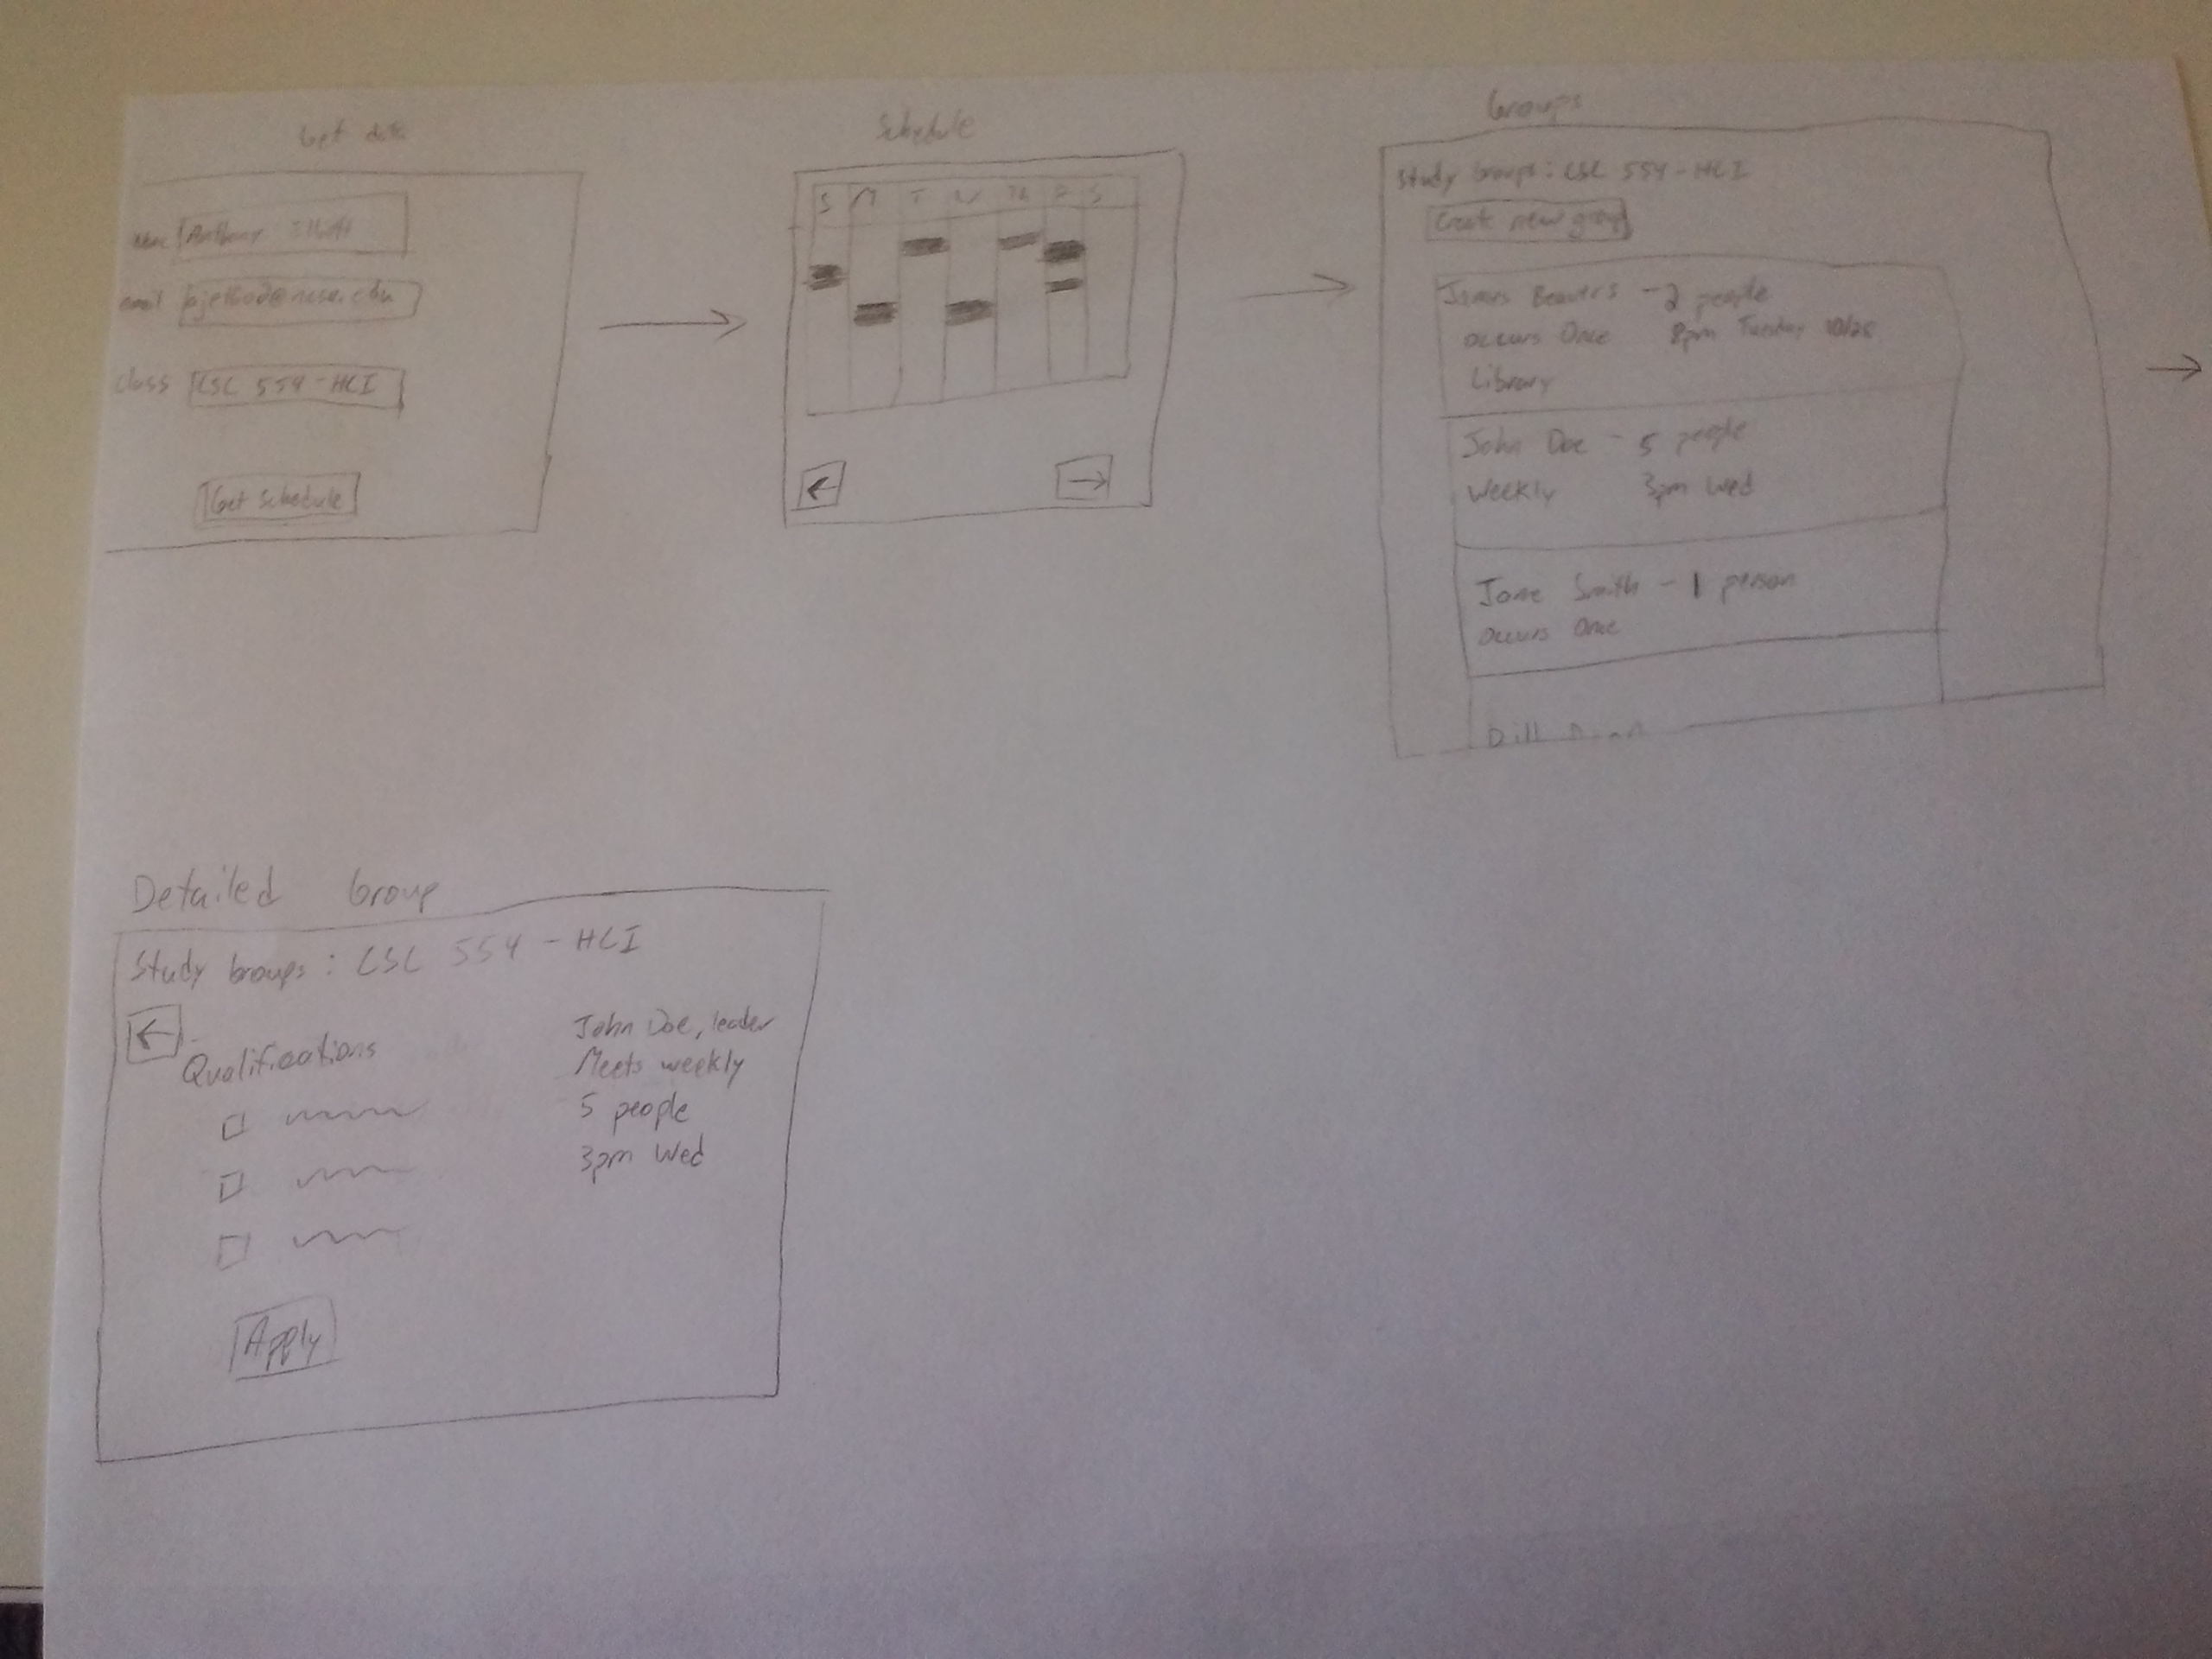
\includegraphics[width=80mm]{figures/flow}
\caption{Shows the flow of the different screens. \label{fig:flow}}
\end{figure}

\begin{figure}[Hht!]
\centering
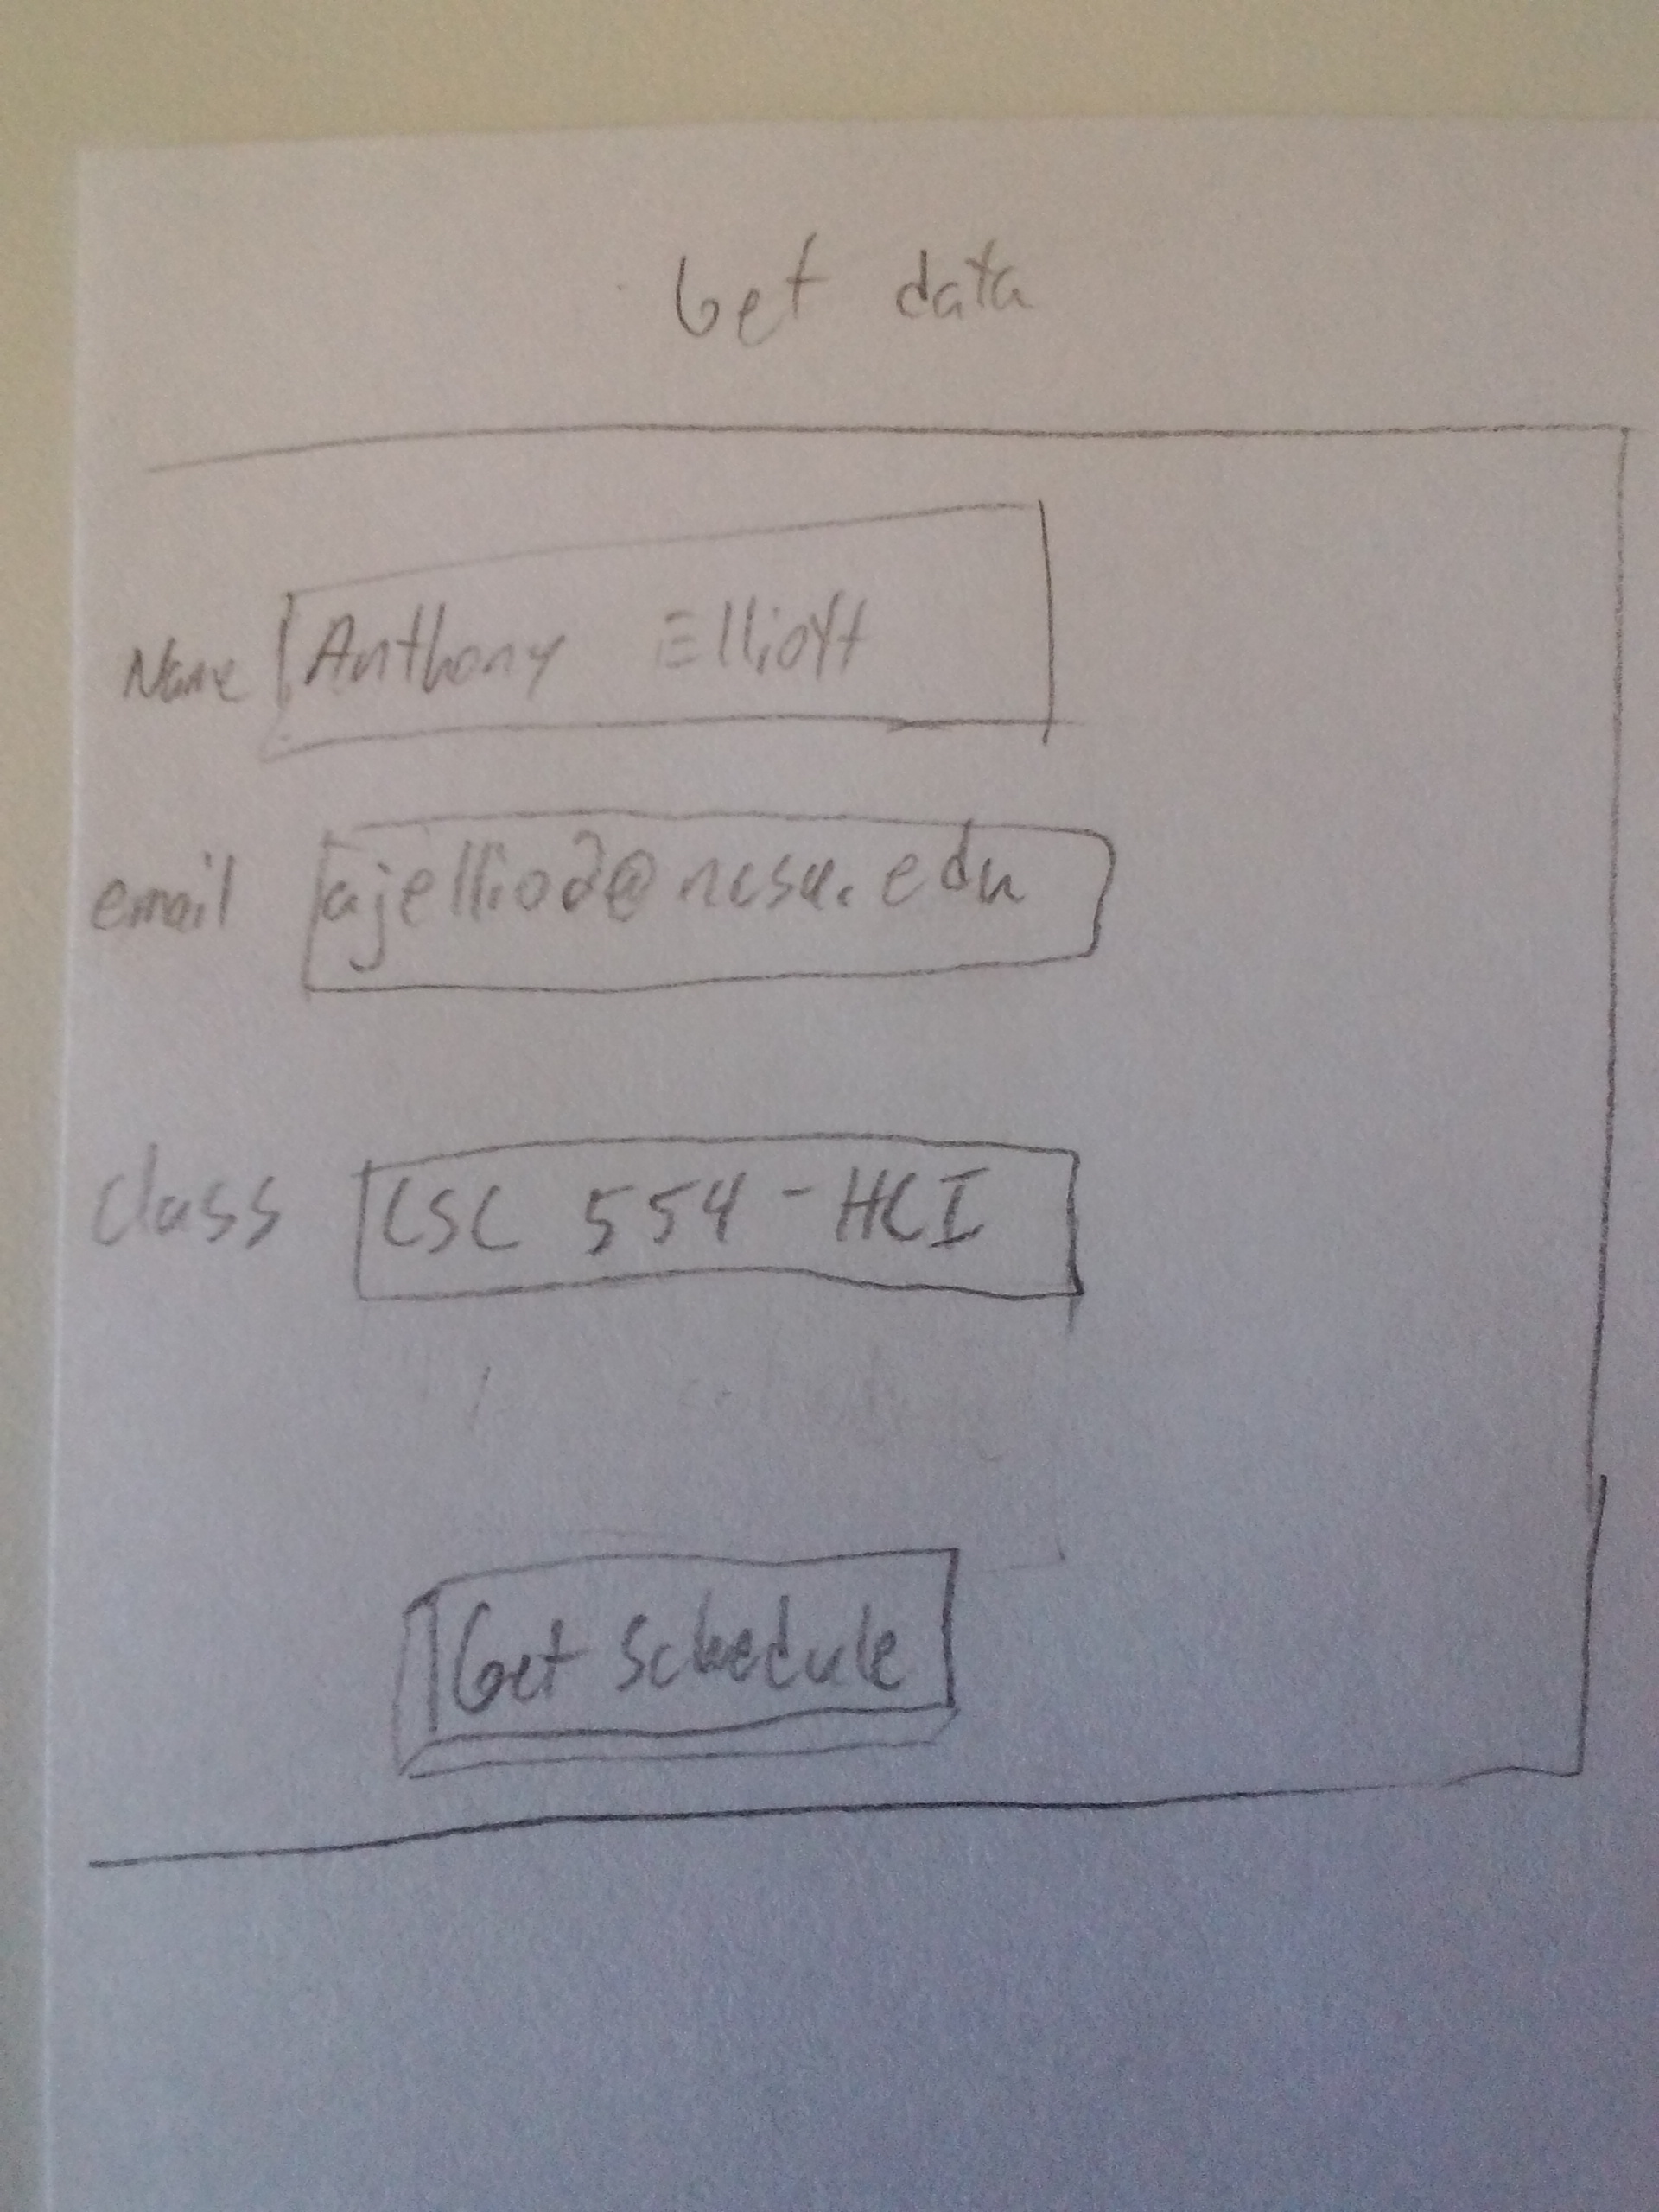
\includegraphics[width=80mm]{figures/getUserData}
\caption{Screen to get user data. \label{fig:userData}}
\end{figure}

\begin{figure}[ht!]
\centering
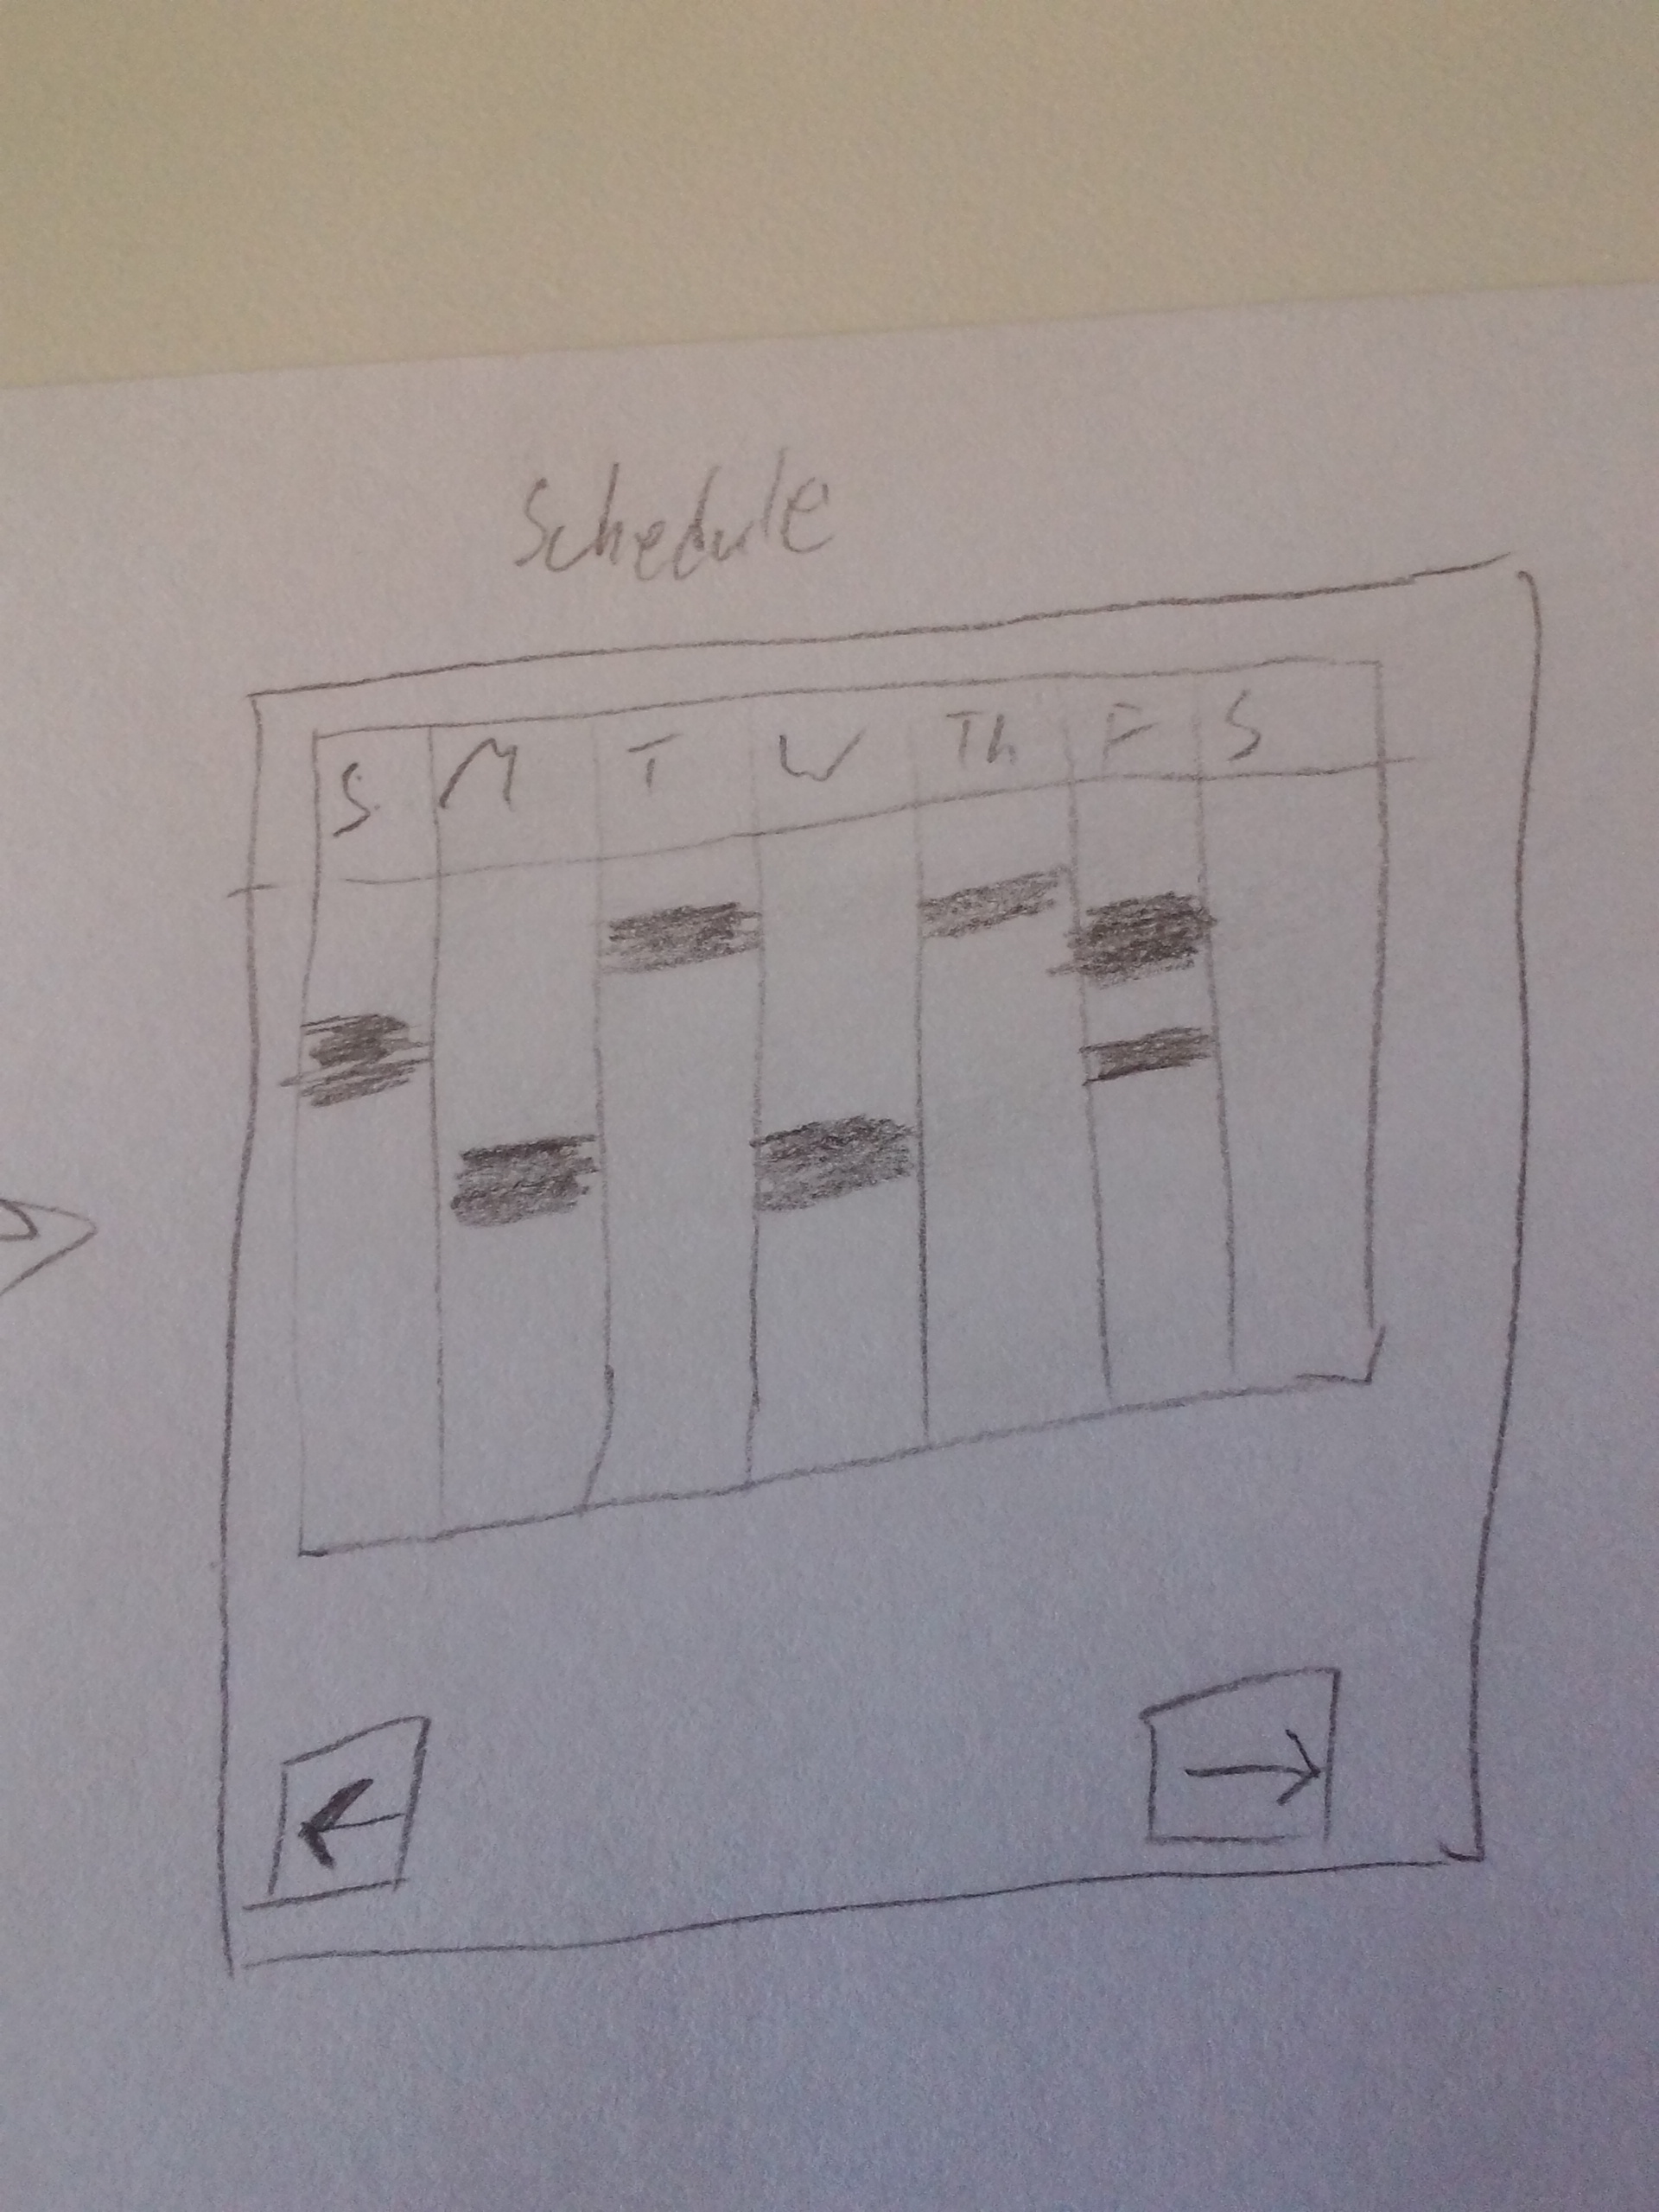
\includegraphics[width=80mm]{figures/schedule}
\caption{Shows the user's schedule. \label{fig:schedule}}
\end{figure}

\begin{figure}[ht!]
\centering
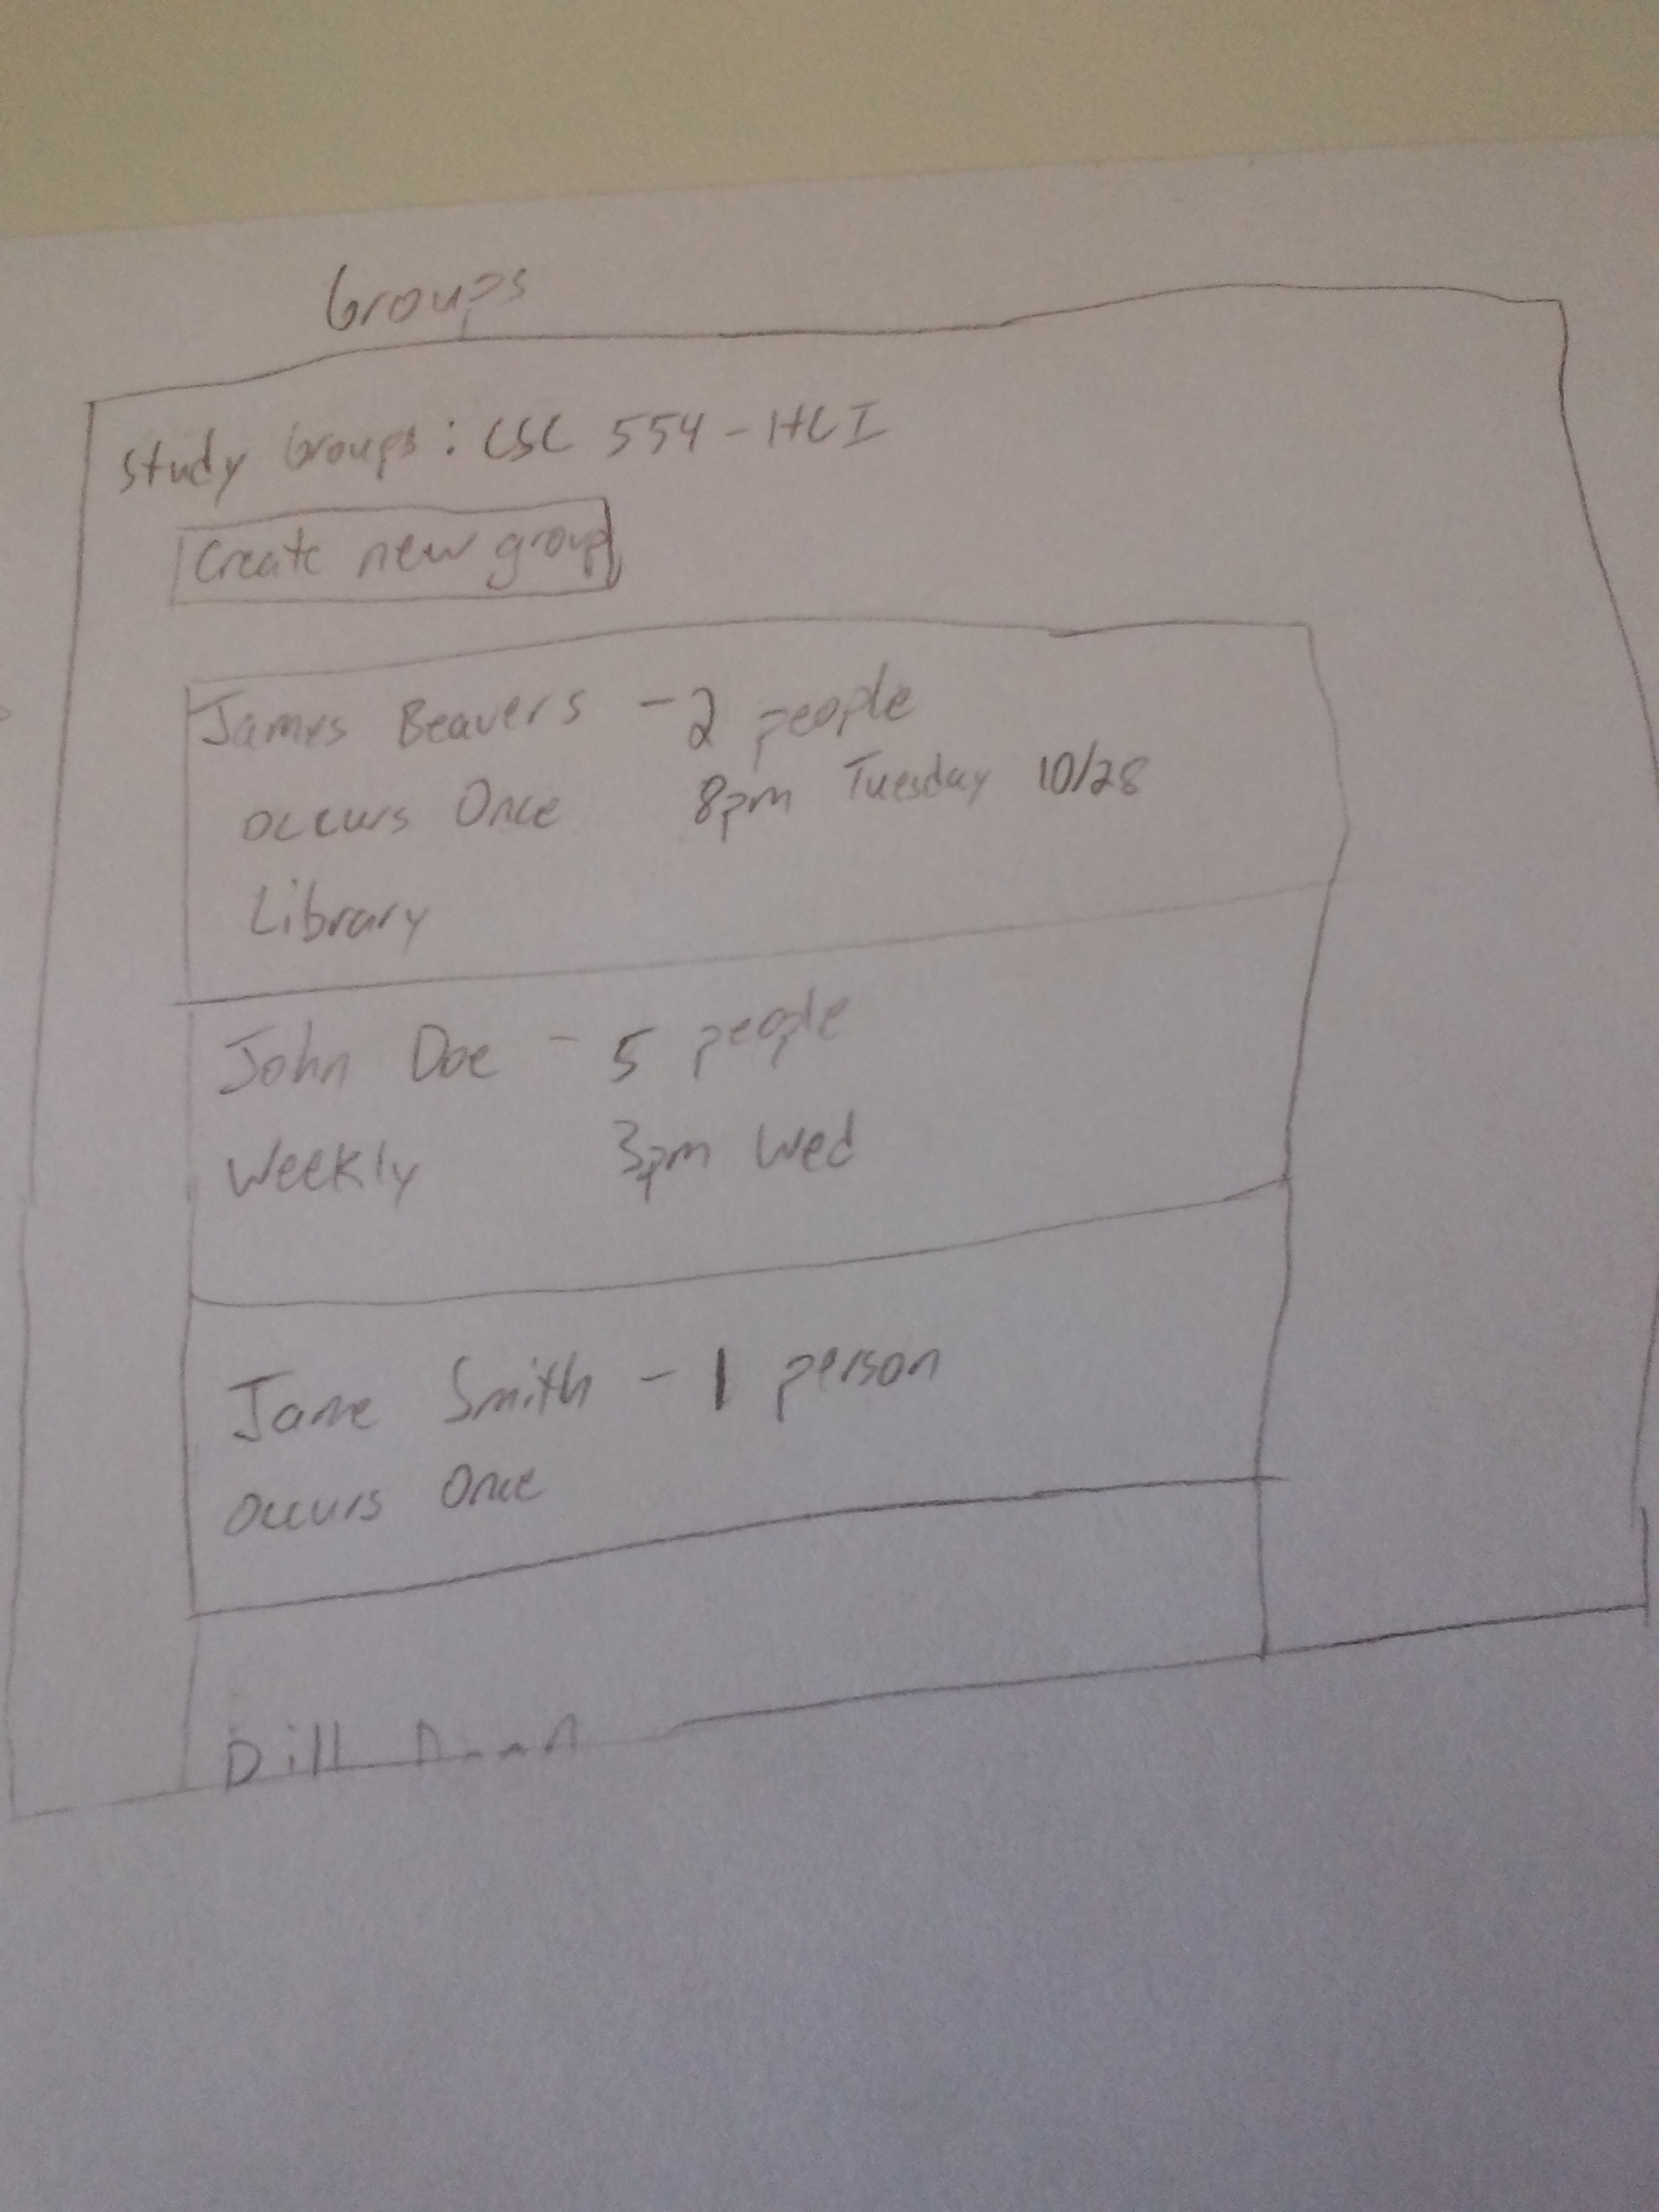
\includegraphics[width=80mm]{figures/groups}
\caption{Lists all groups. \label{fig:groups}}
\end{figure}

\begin{figure}[ht!]
\centering
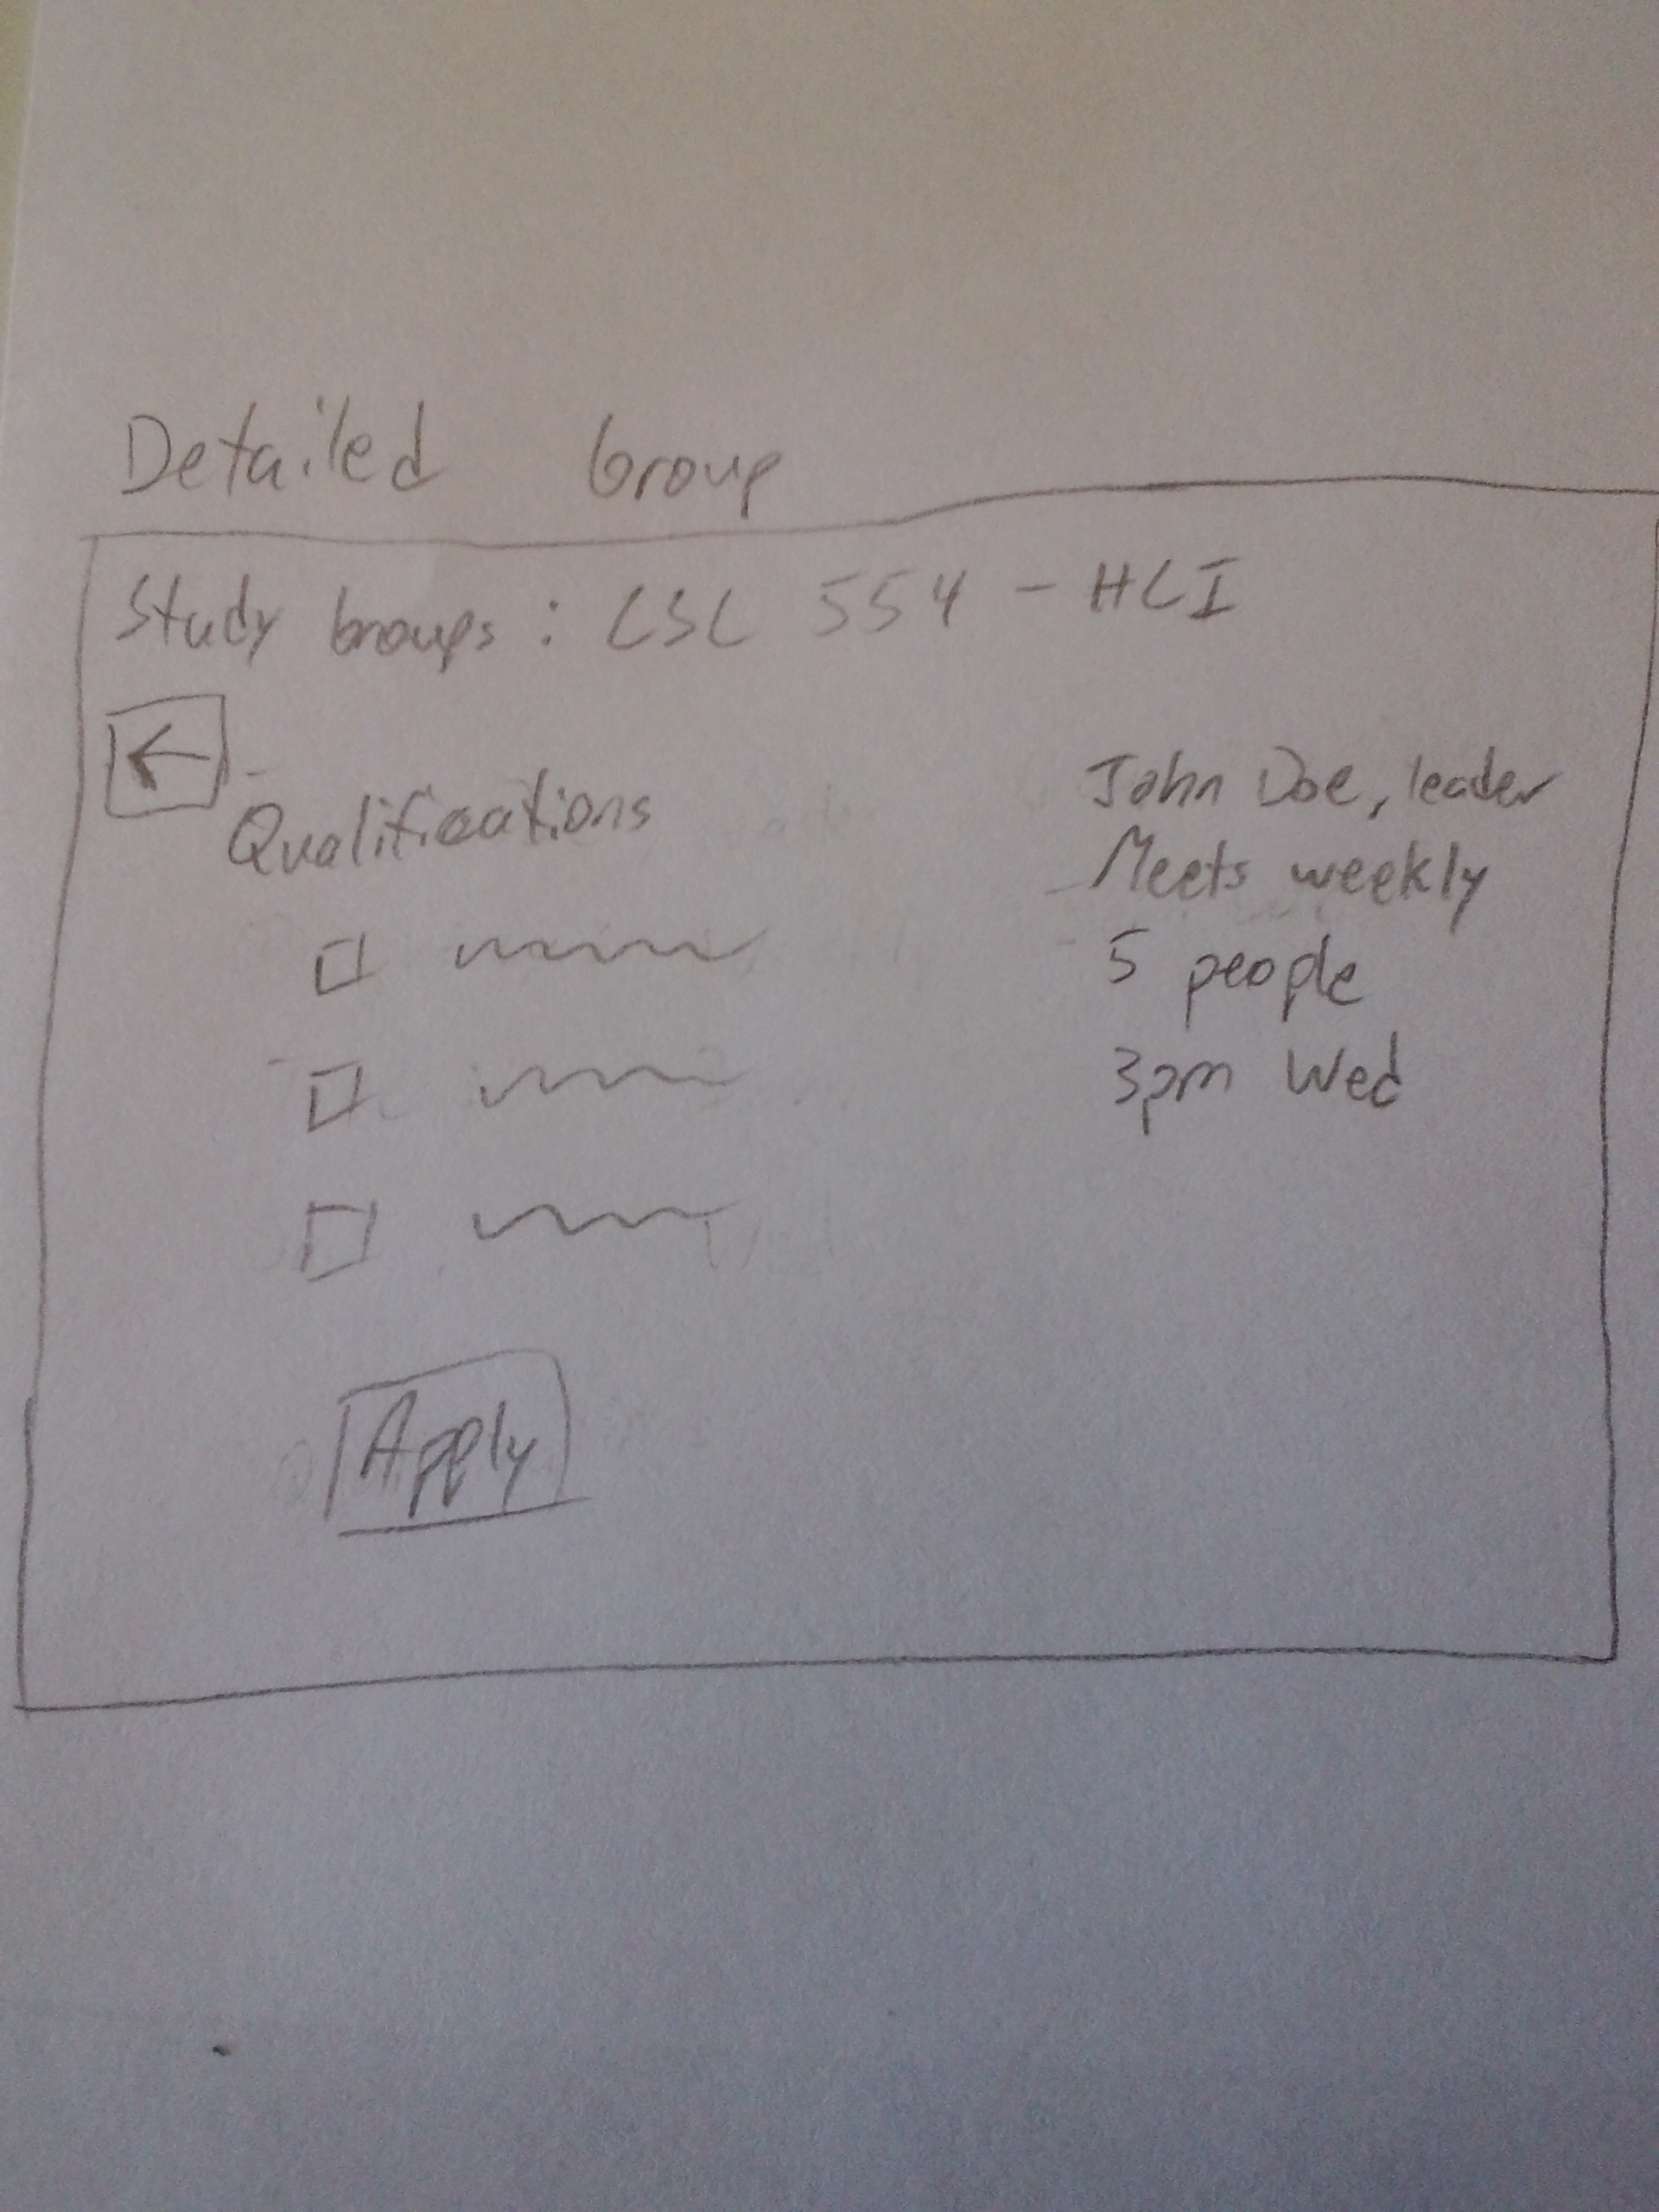
\includegraphics[width=80mm]{figures/detailedGroup}
\caption{Shows the detailed view of one group. \label{fig:detailedGroup}}
\end{figure}

\begin{figure}[ht!]
\centering
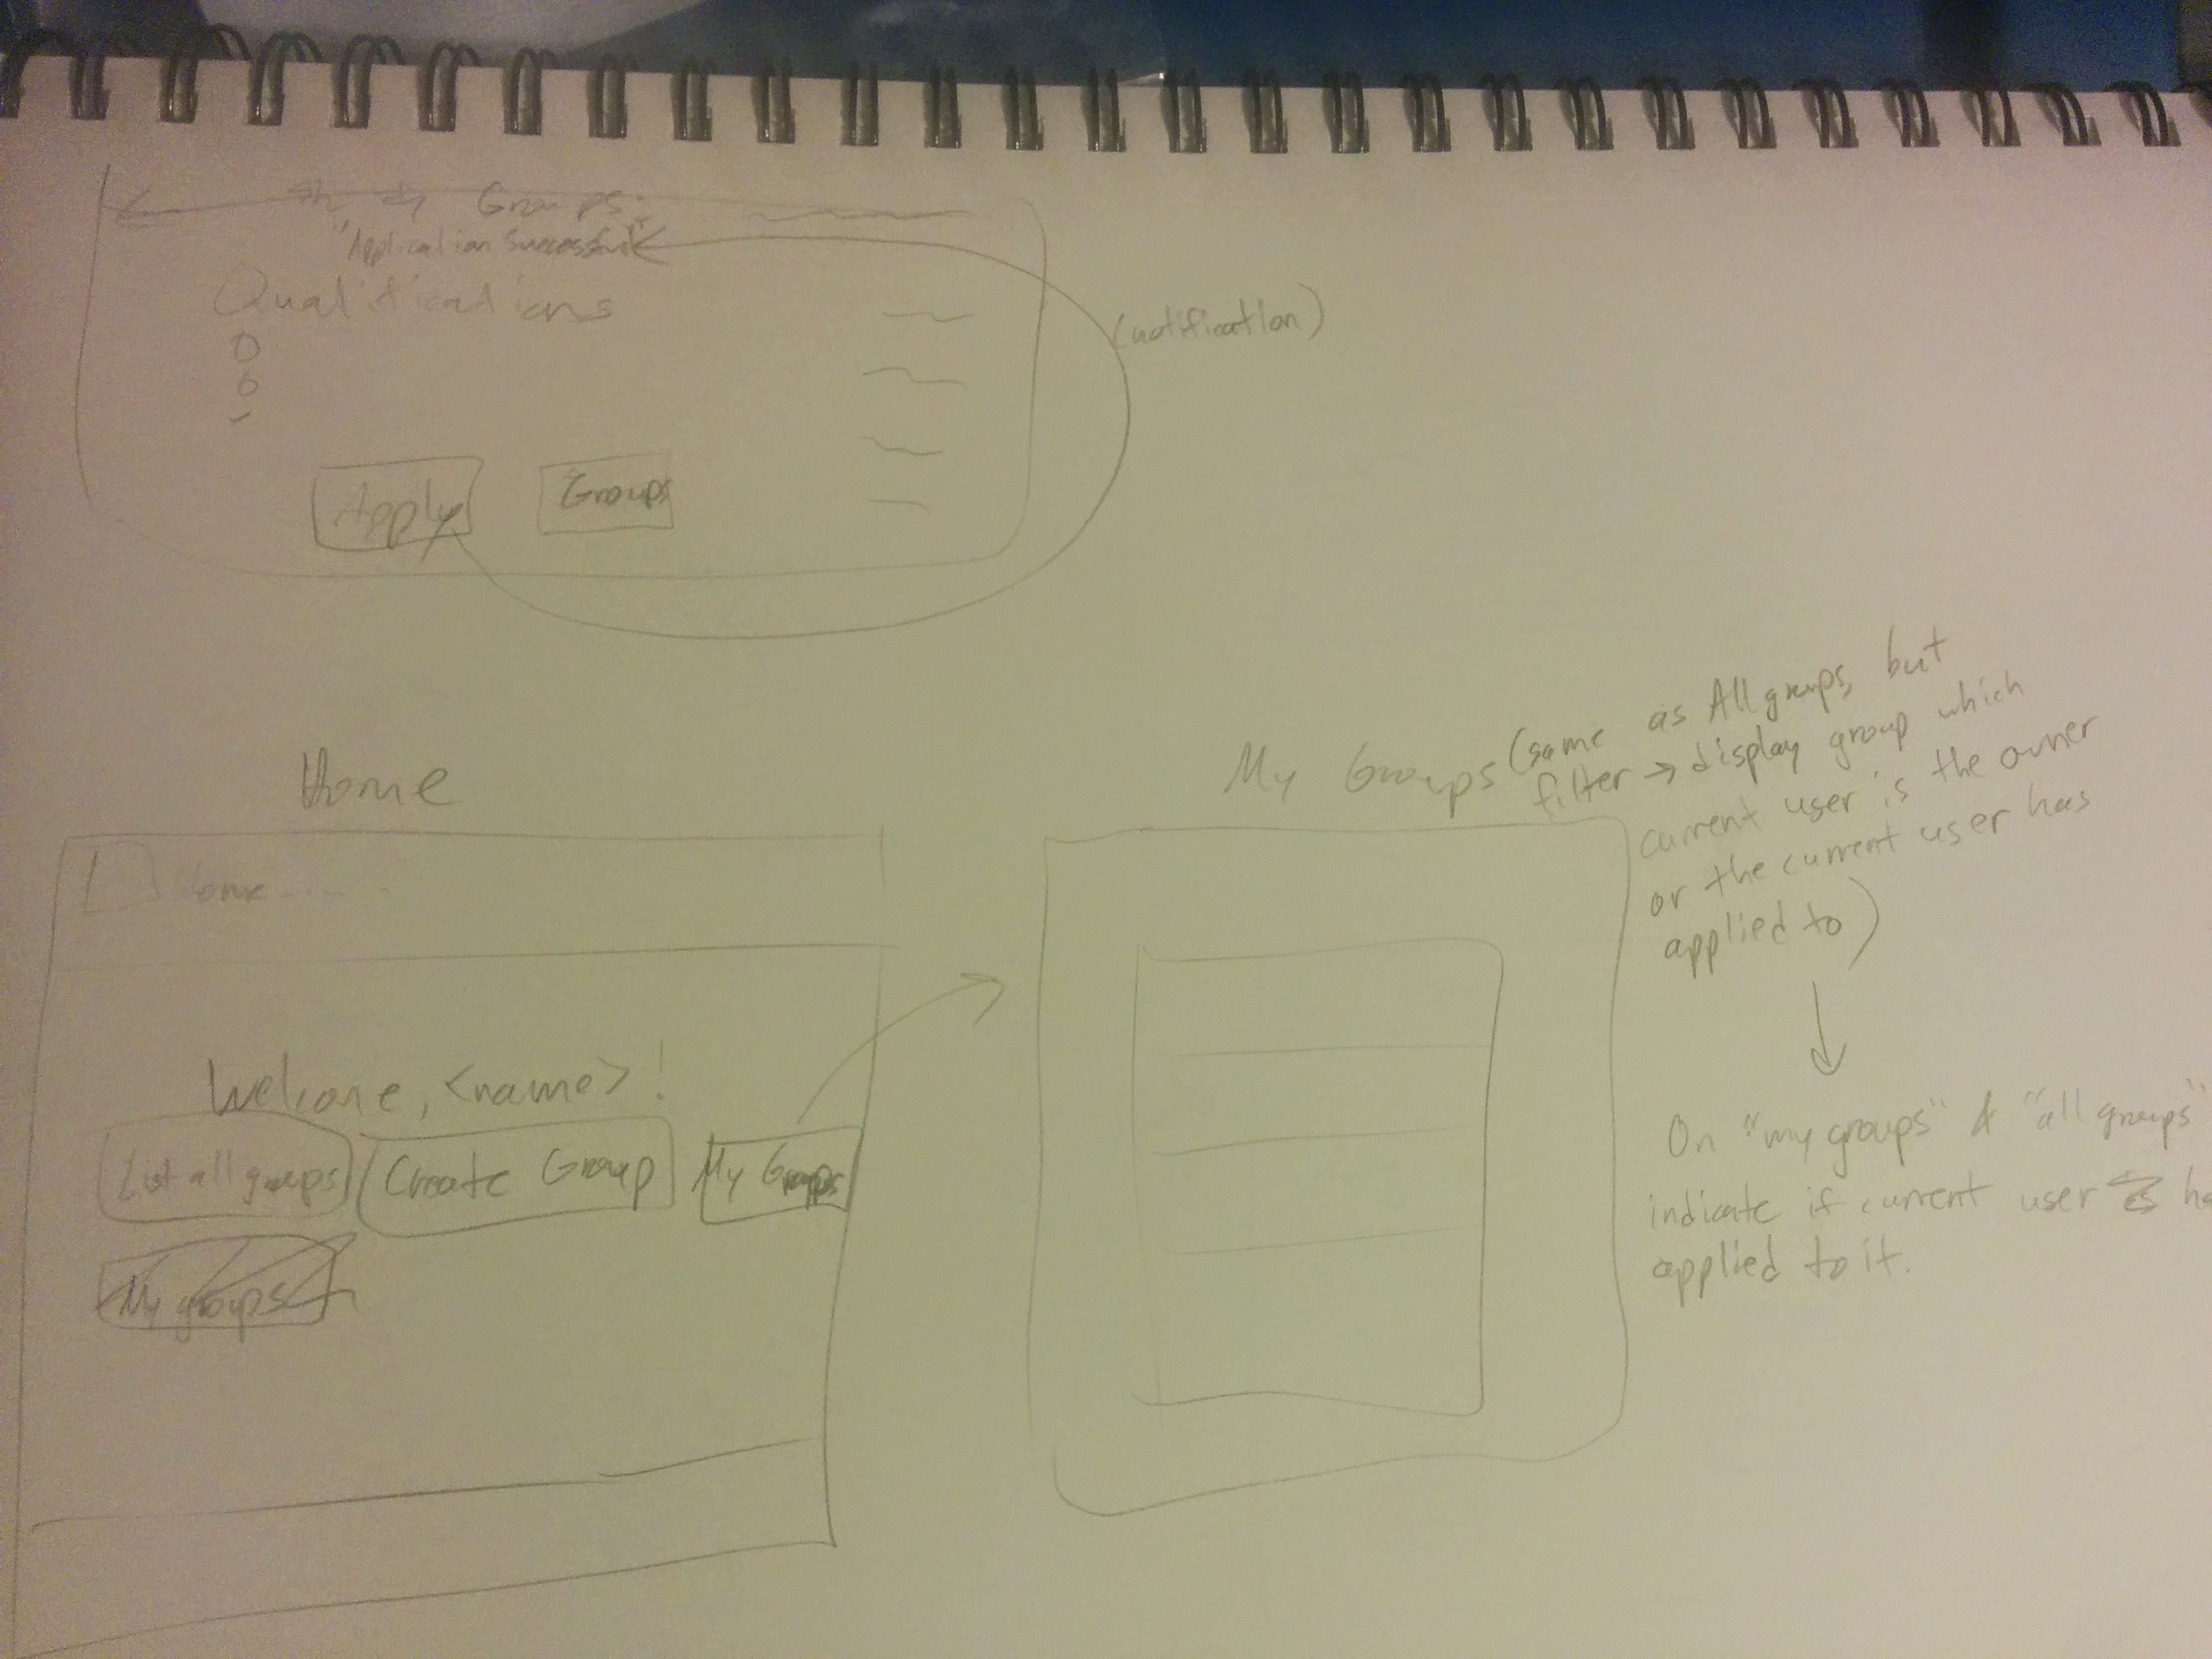
\includegraphics[width=80mm]{figures/applyandGroupsFlowSketch}
\caption{Shows the group apply button and flow of viewing groups of which the user is a member. \label{fig:applyandGroupsFlowSketch}}
\end{figure}

\begin{figure}[ht!]
\centering
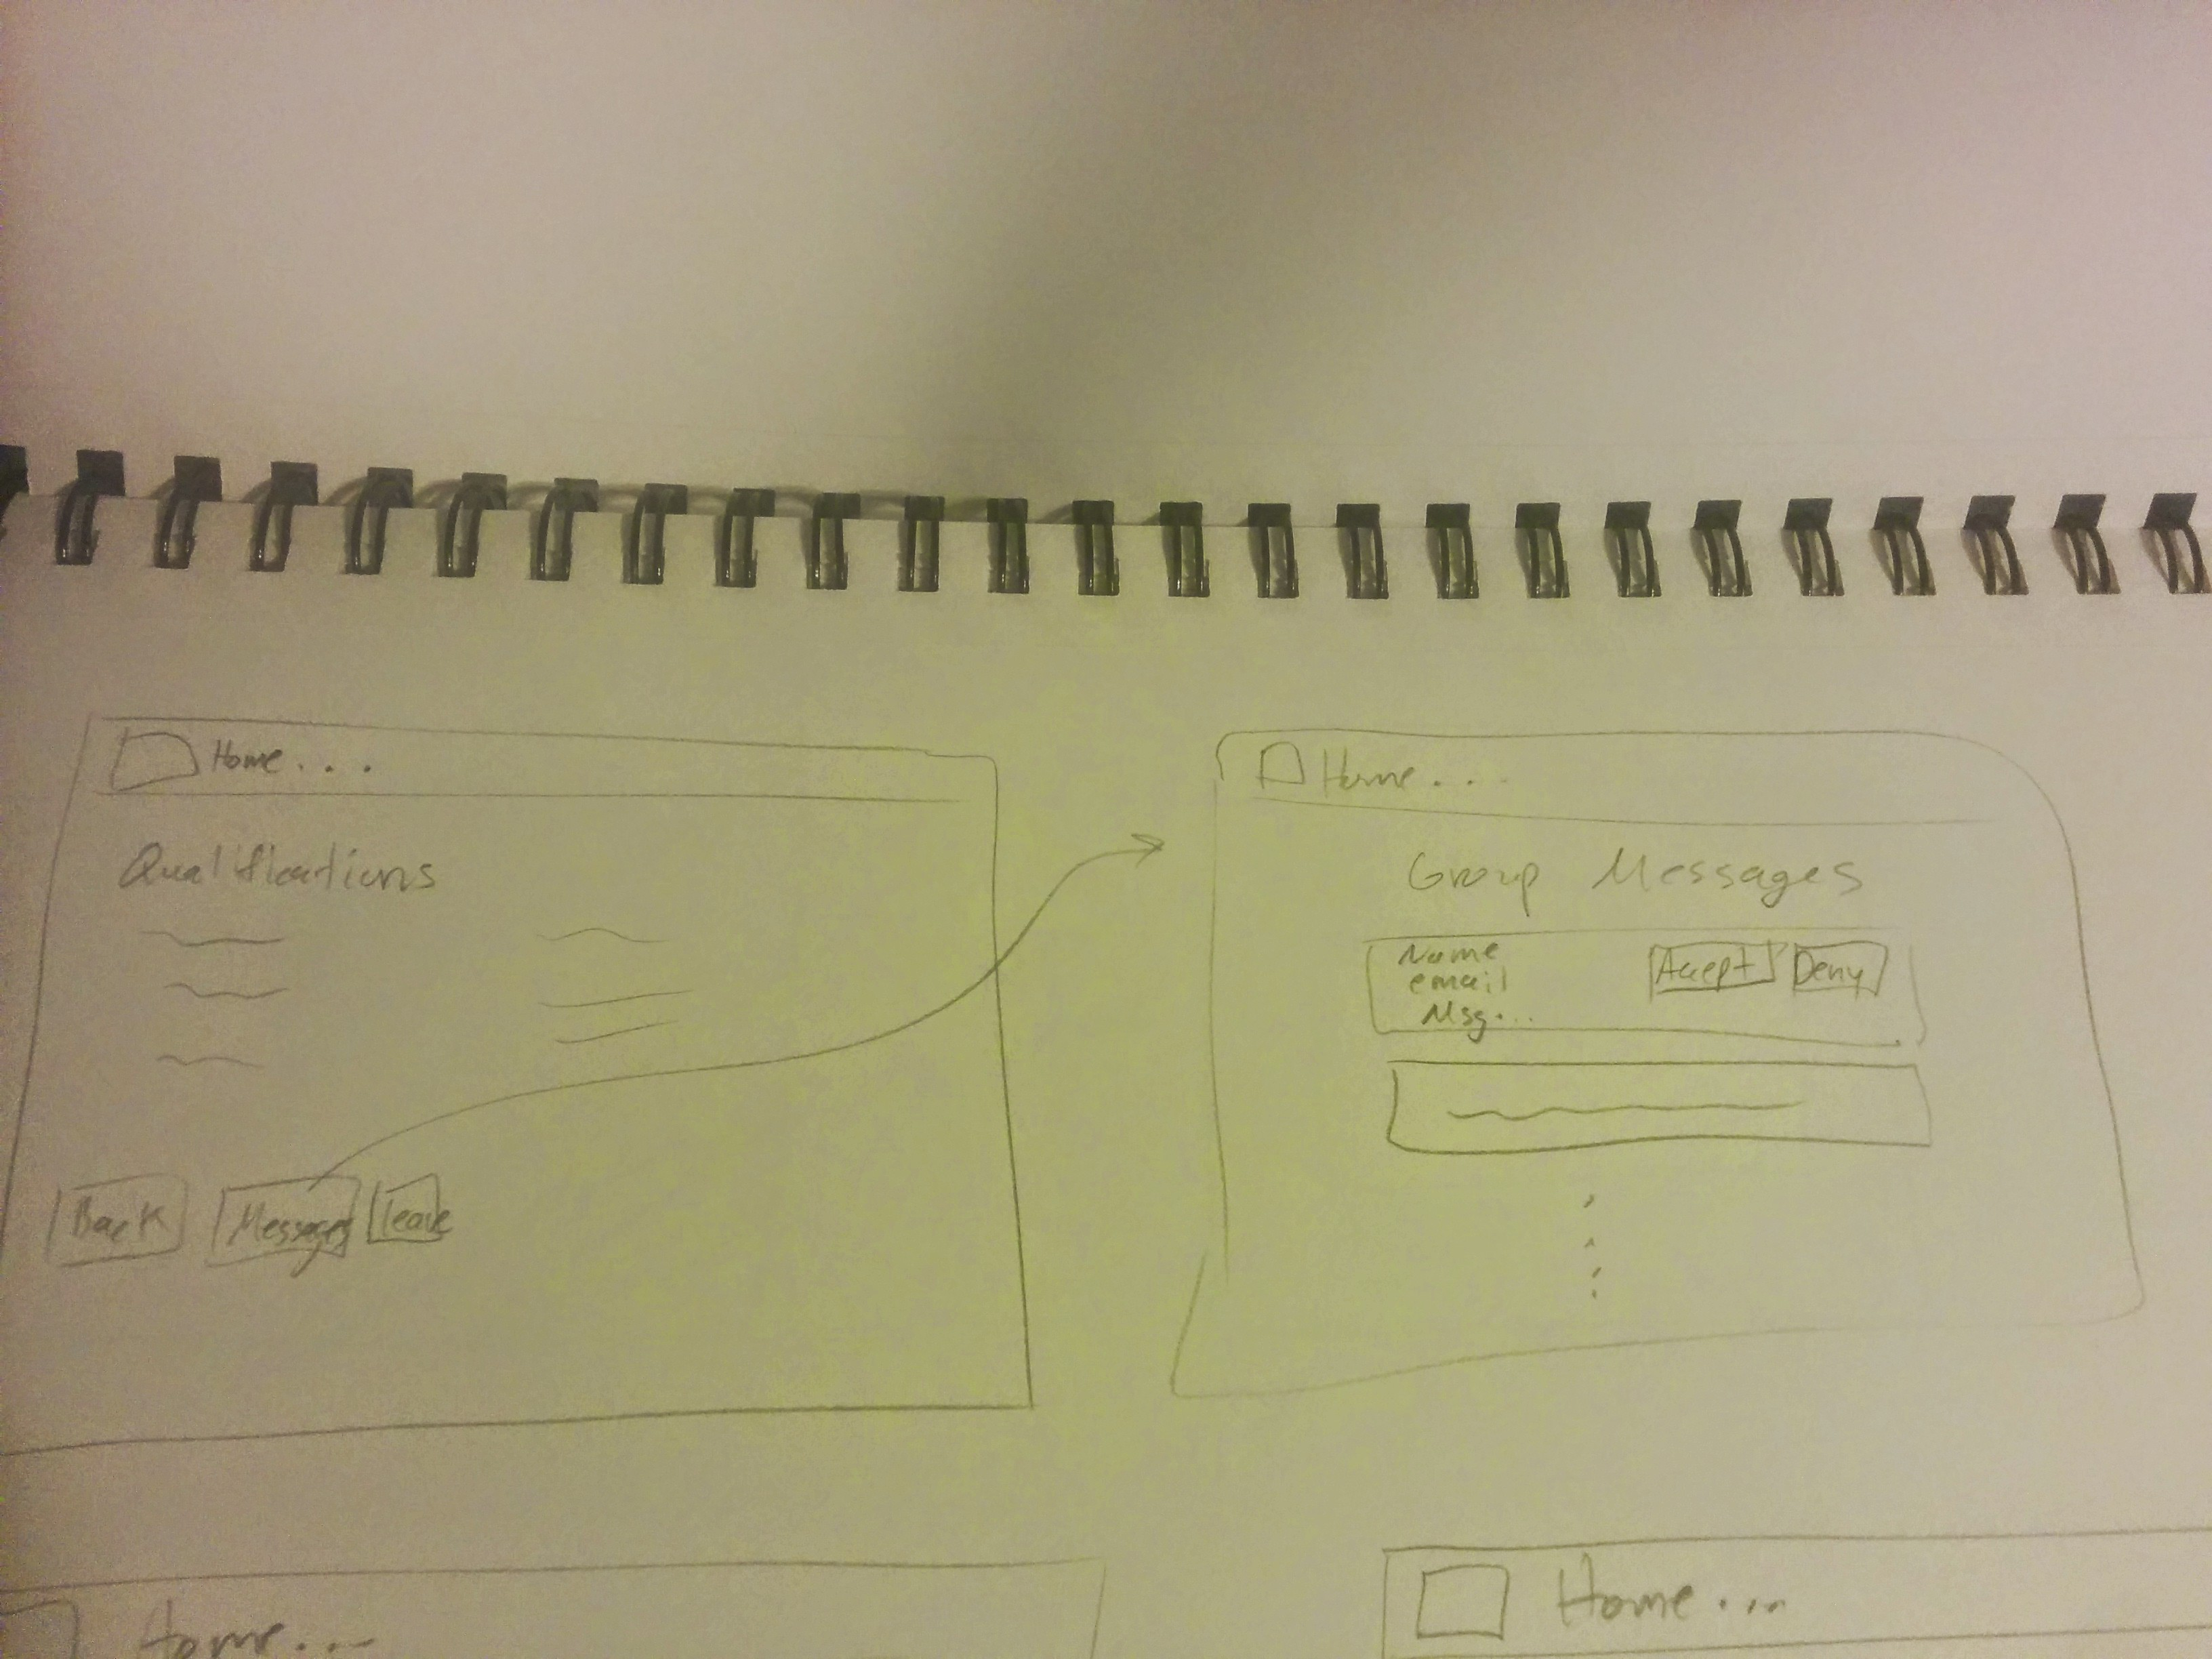
\includegraphics[width=80mm]{figures/messagesSketch}
\caption{Flow of viewing group messages. \label{fig:messagesSketch}}
\end{figure}

\begin{figure}[ht!]
\centering
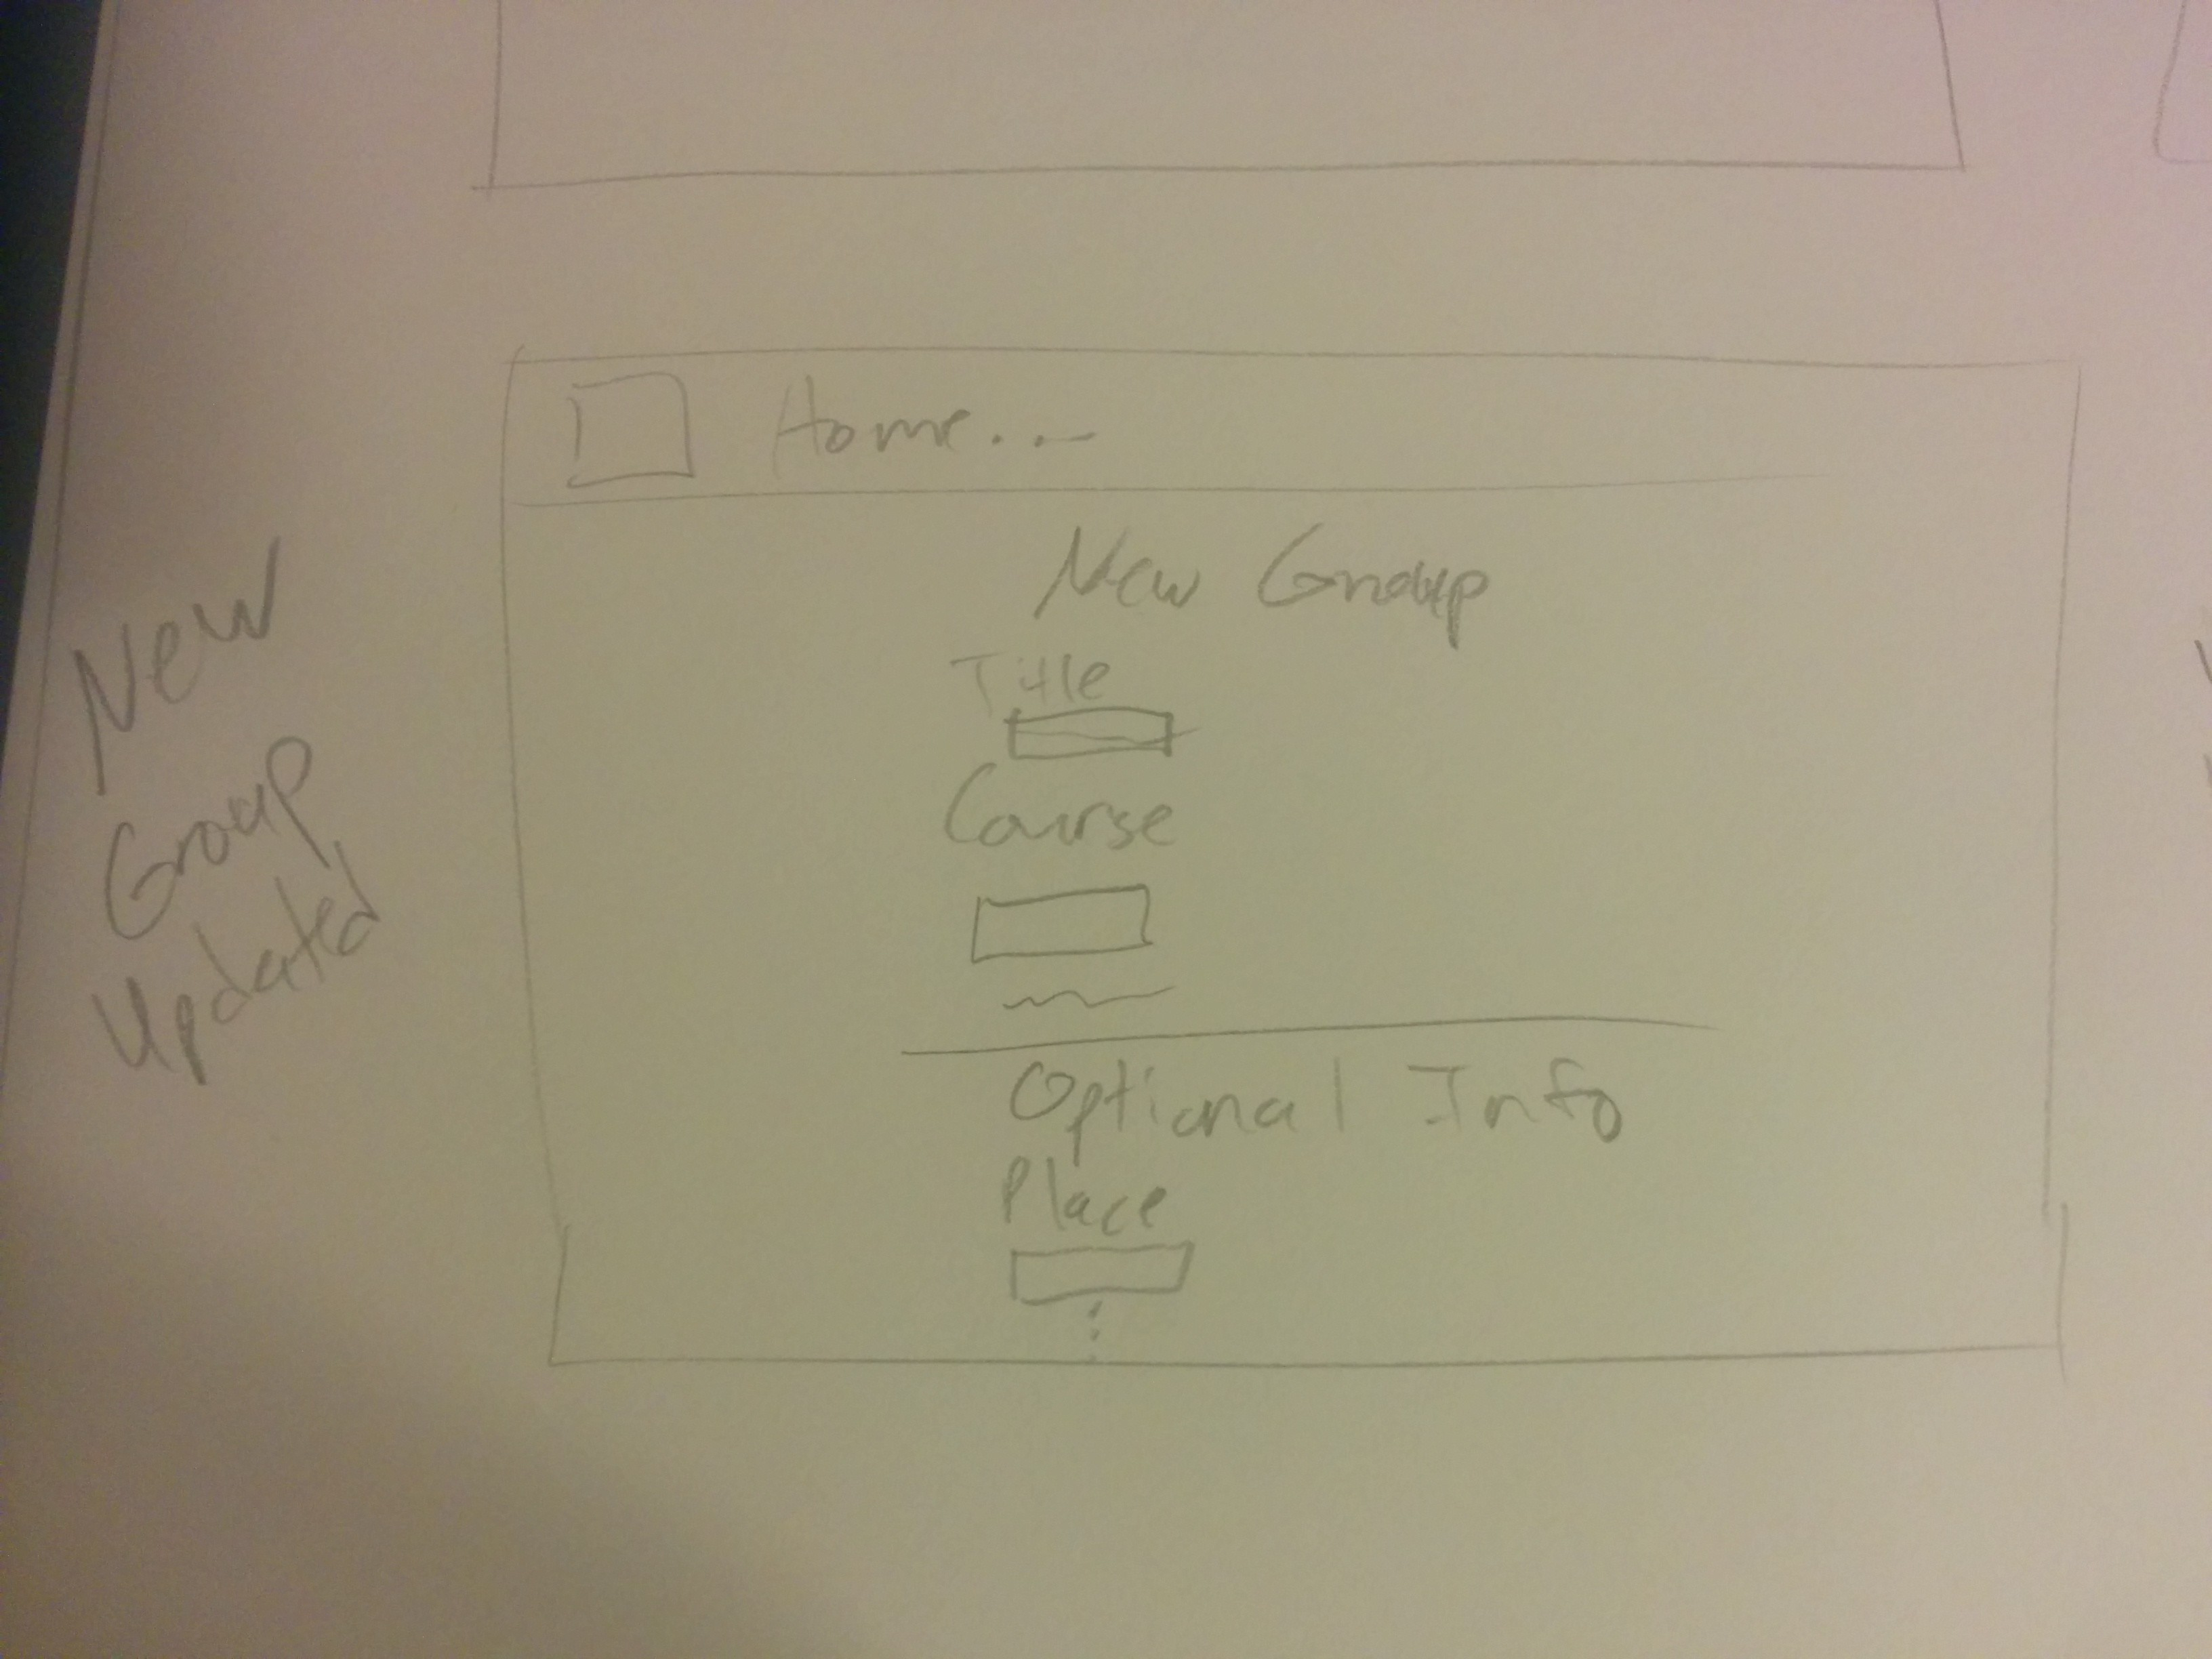
\includegraphics[width=80mm]{figures/newGroupSketch}
\caption{Group creation view (Updated version) \label{fig:newGroupSketch}}
\end{figure}

\begin{figure}[ht!]
\centering
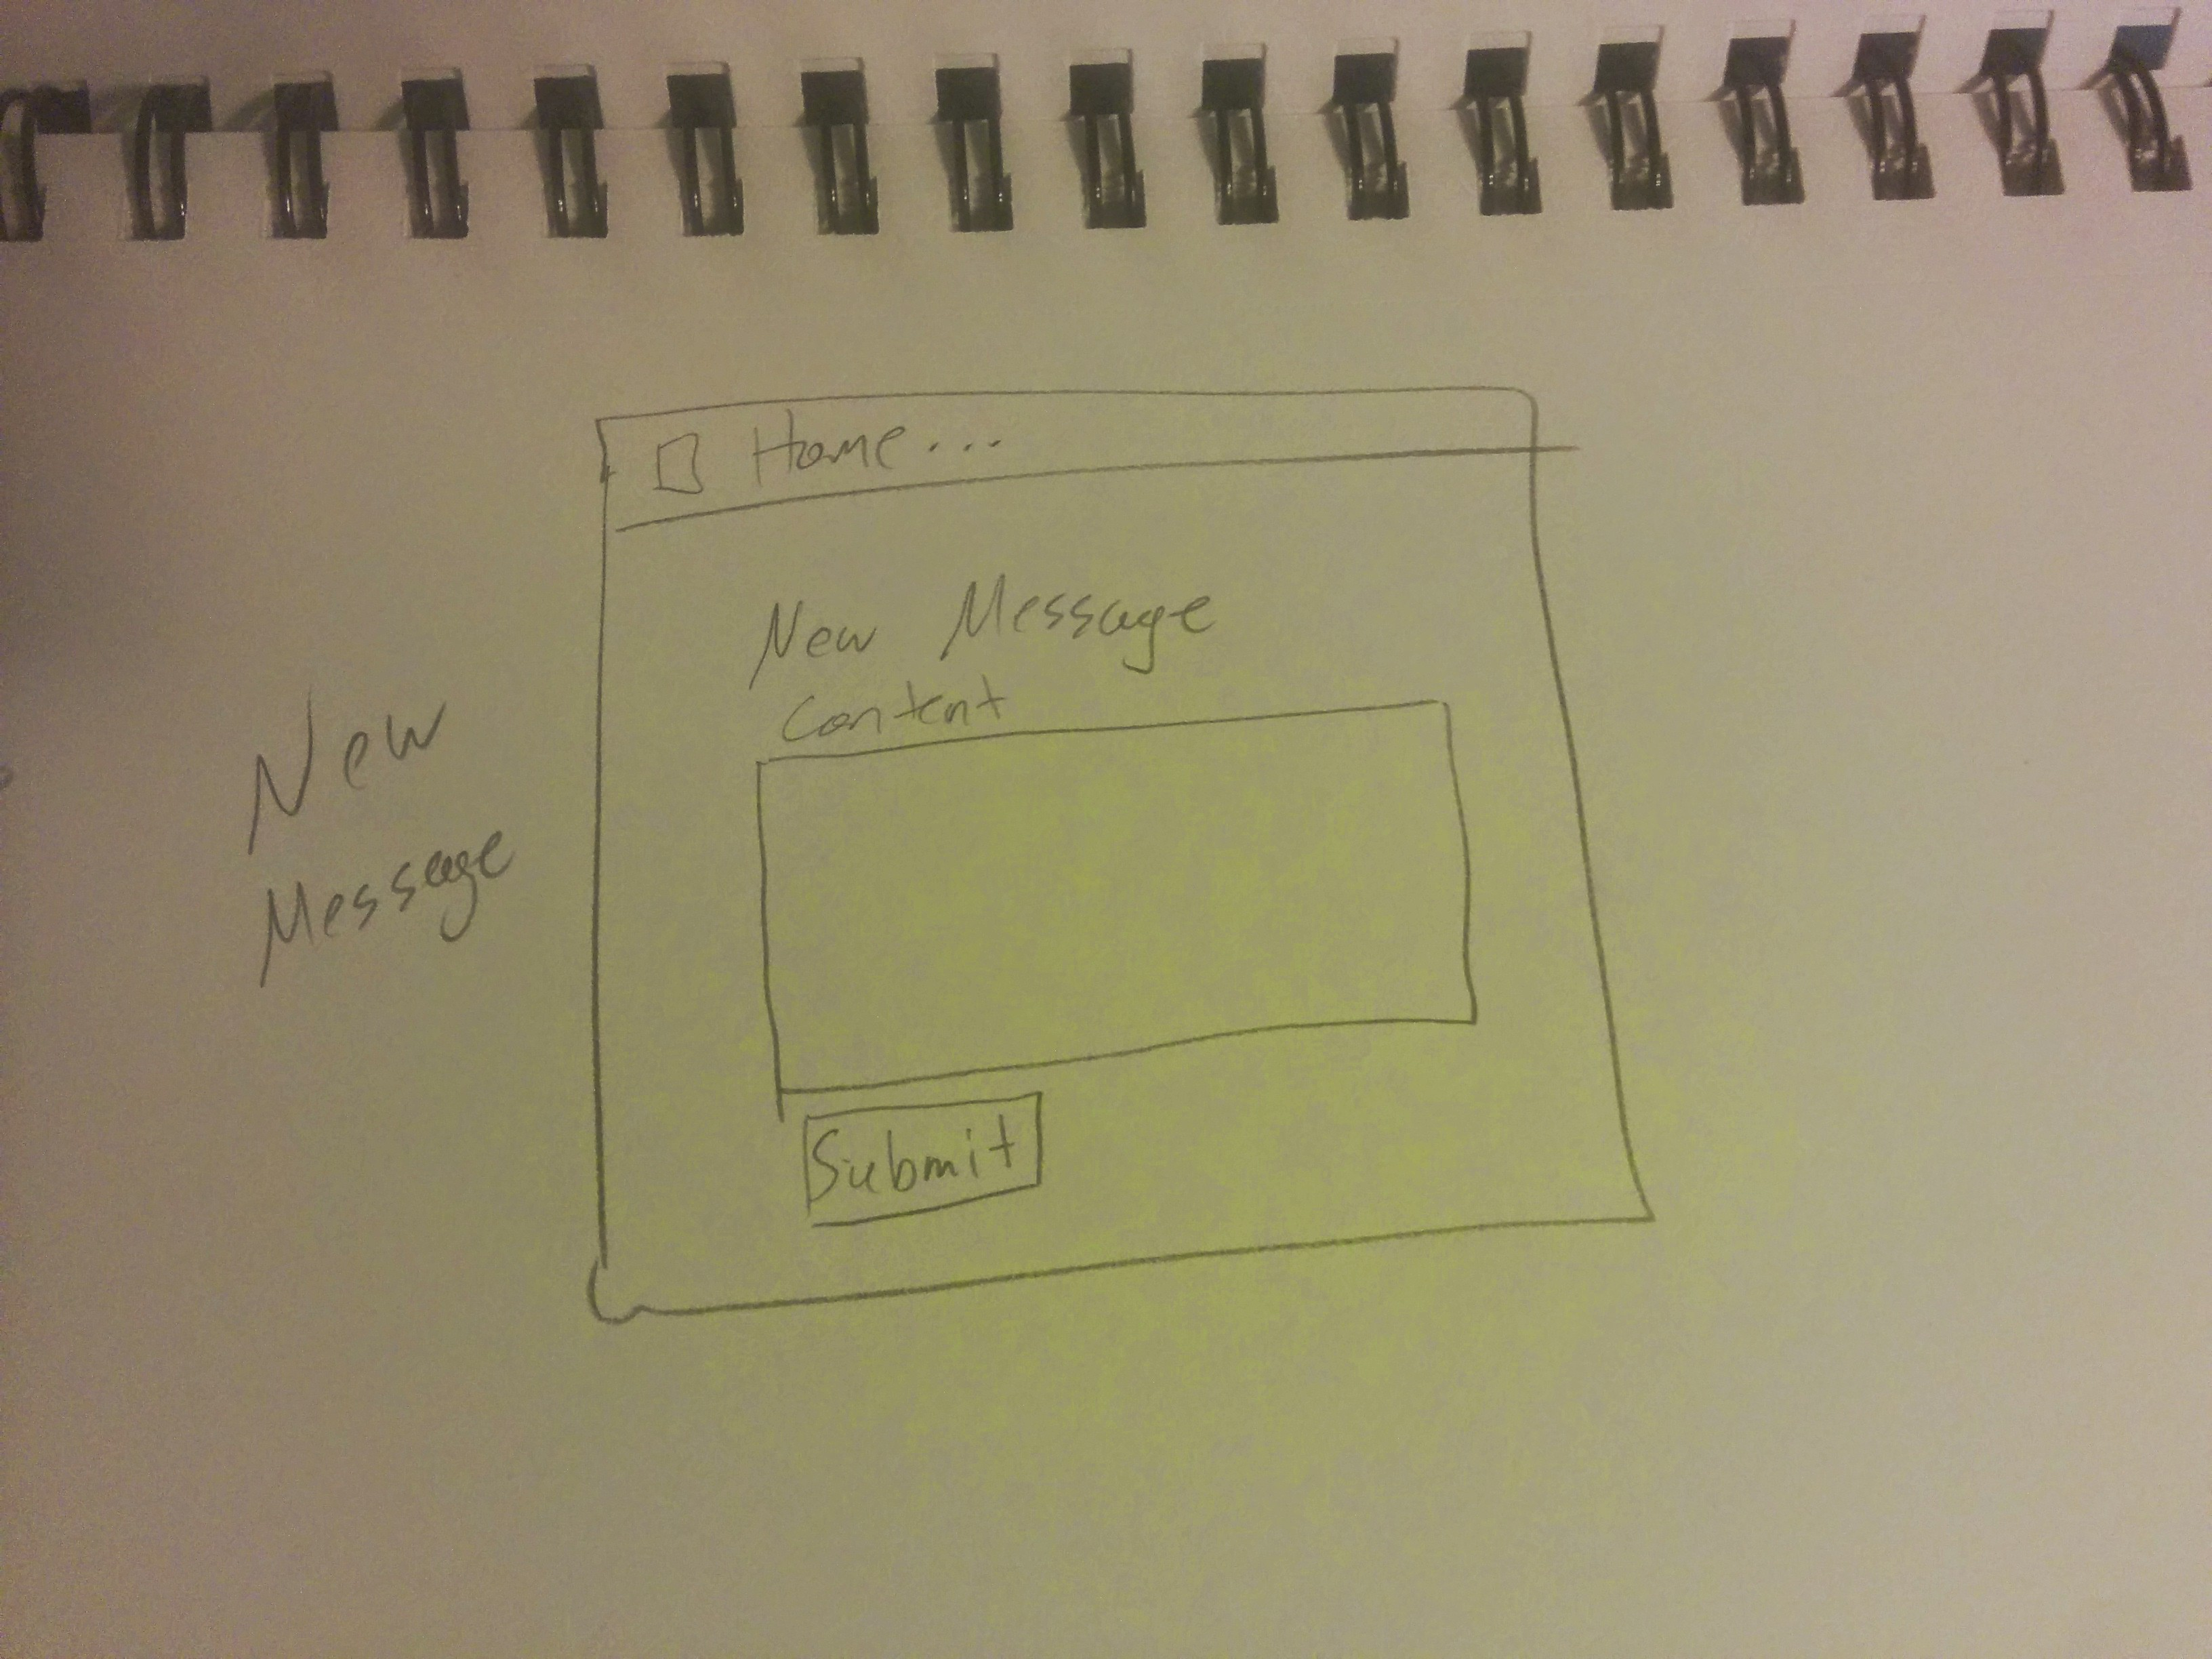
\includegraphics[width=80mm]{figures/newMessageSketch}
\caption{Group message creation view
\label{fig:newMessageSketch}}
\end{figure}

\begin{figure}[ht!]
\centering
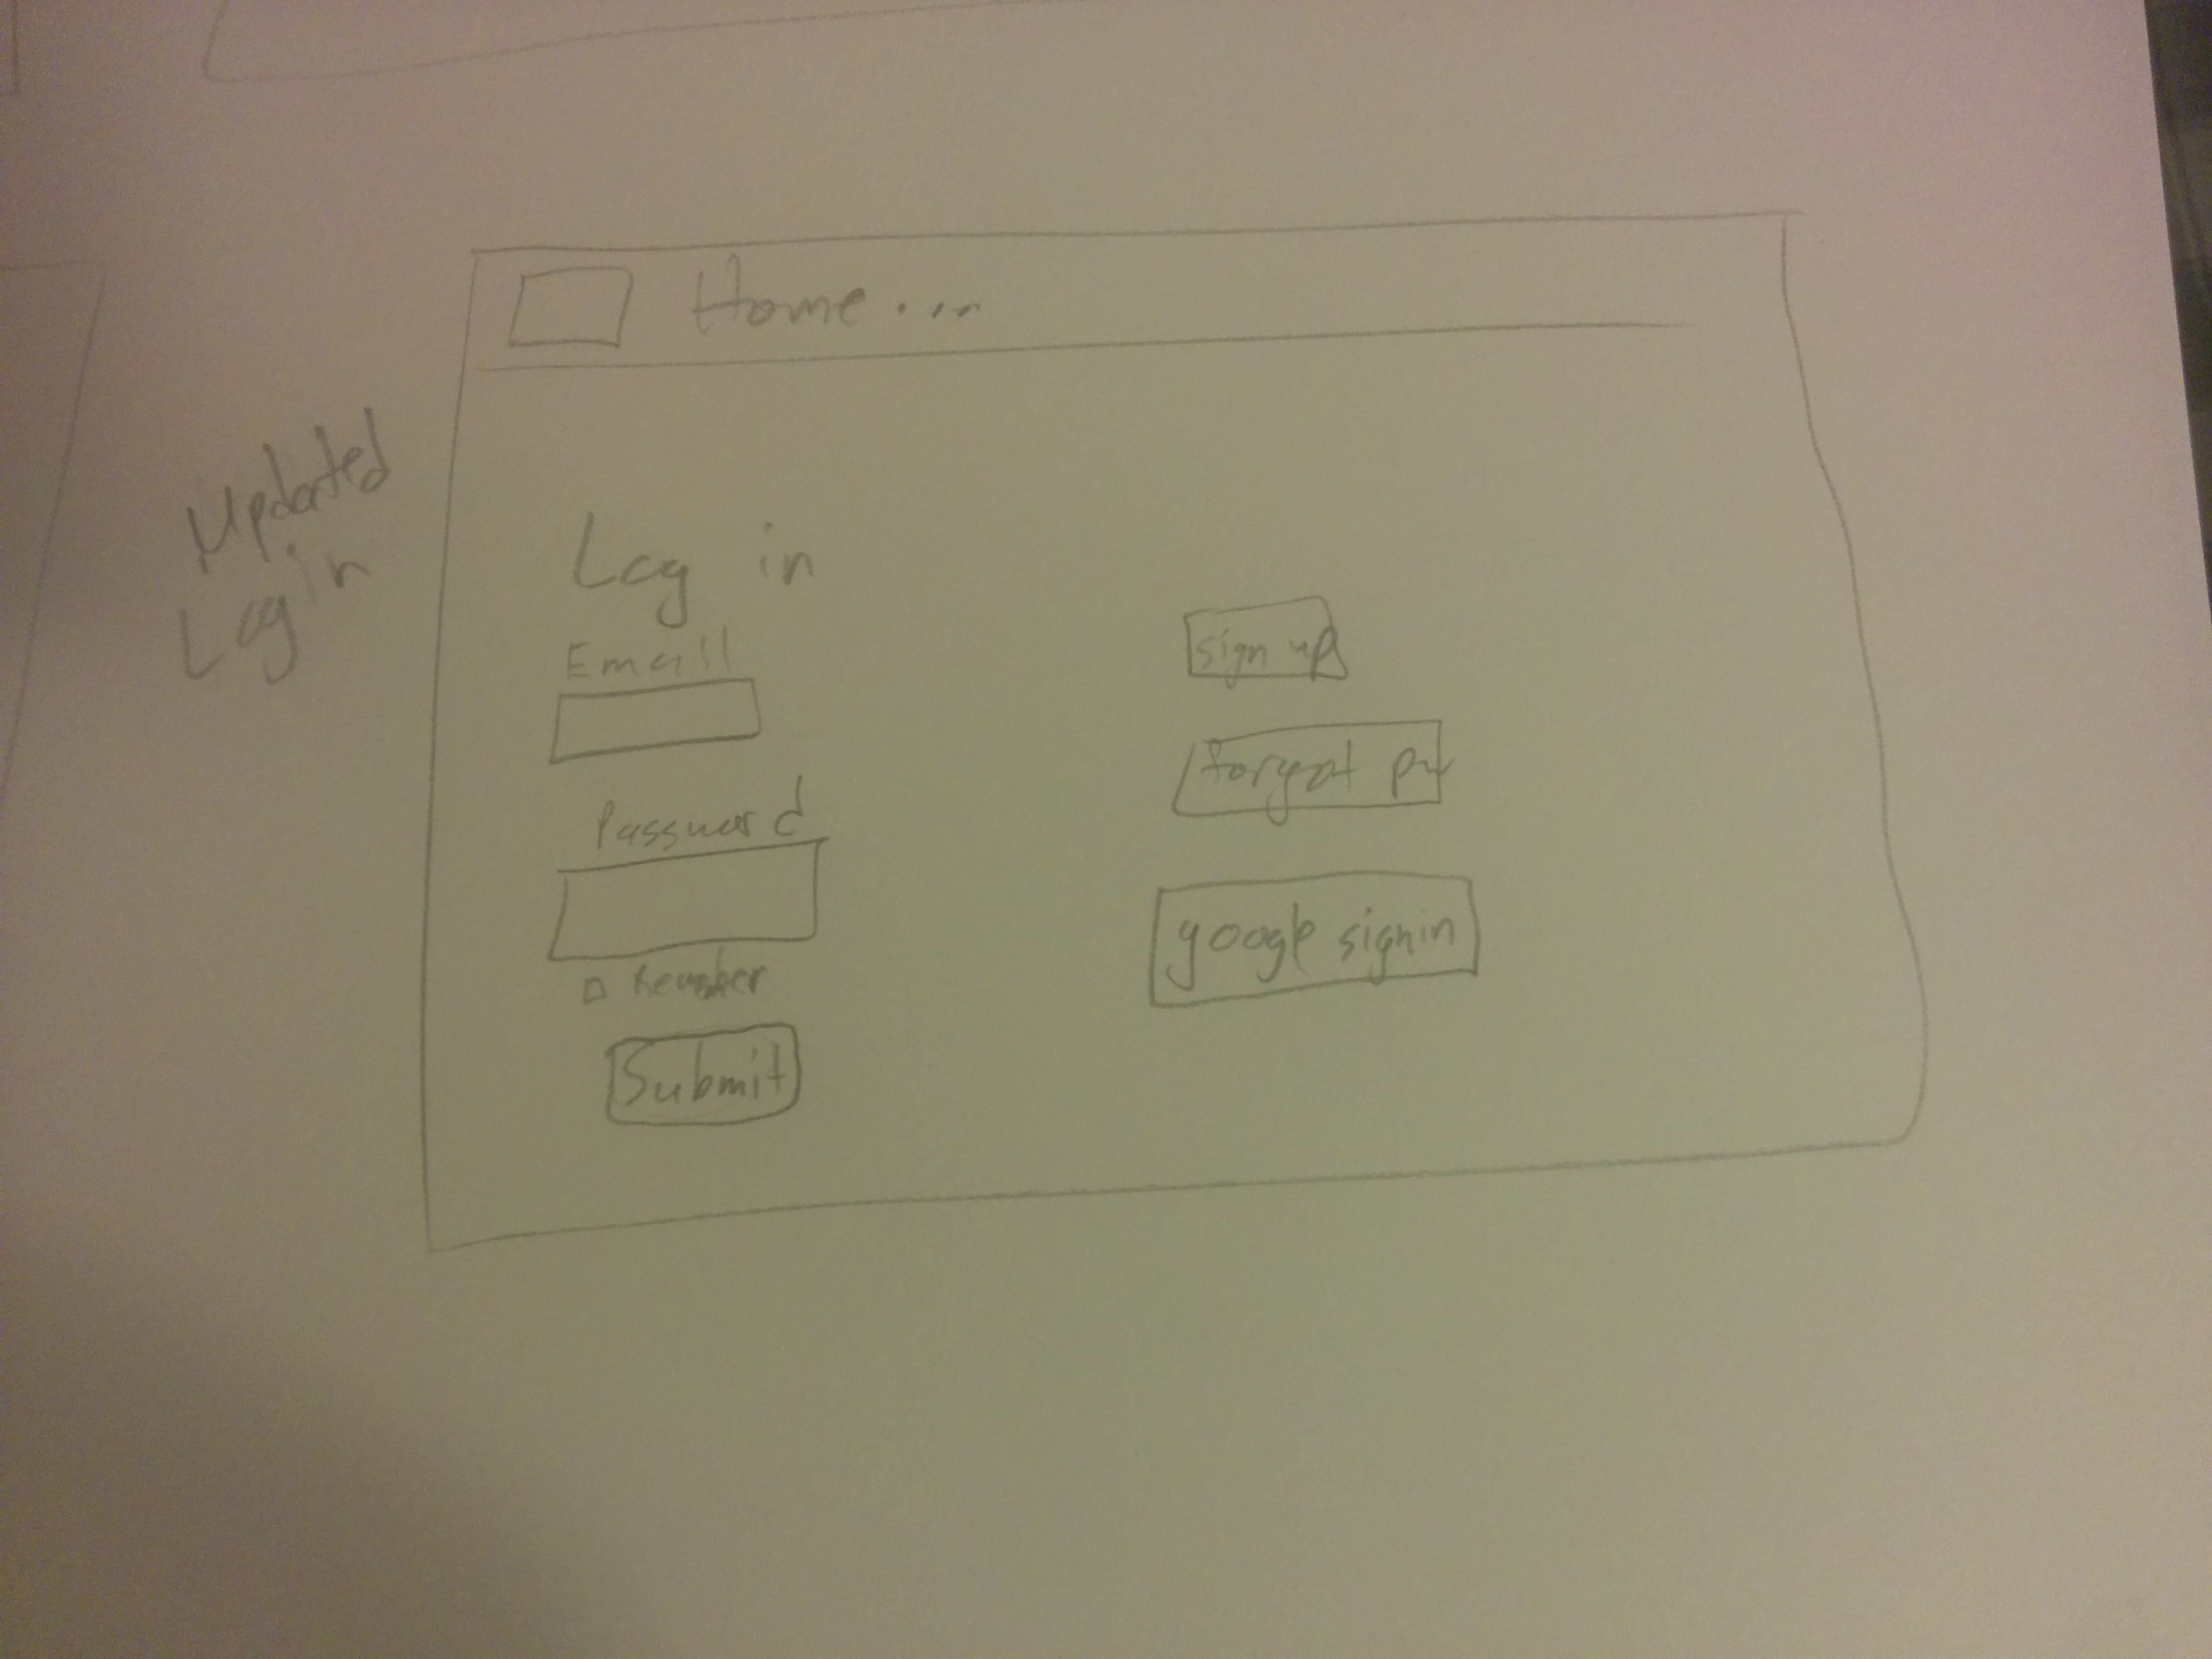
\includegraphics[width=80mm]{figures/updatedLoginSketch}
\caption{Login screen (Updated version)
\label{fig:updatedLoginSketch}}
\end{figure}

\section{Interview Notes}
\textbf{Overview}
Looking at two different types of tools. One tool could be a `matchmaking' tool that helps to form the groups themselves. The other type is to assist study groups that have already been formed.

Neither of the interviewees thought that they would actually use a matchmaking tool. But they did like the tool that would assist the already formed group.

Could these two be combined?

Homework study groups are different than exam study groups.

\textbf{Details}
Helps to do bulk of the studying alone and then use SG to ensure people have the right understanding.

All participants should be at the same level

*helps to work examples together

everyone needs common background.
  are you comfortable with section x ?
  are you an expert on section y ?

personality.
  some people are really distracting and this completely undermines the entire study group.
  some people have an abnormally hard time understanding the material and would drag the group down.
  some people understand it very well and are a big asset to have in a SG.

Group size.
  Level of distraction increases with the number of people in the group.
  2 is ideal, 3 is ok, 4 is pushing it, 5 is almost always bad.
  distractions mean less efficient (more time spent in the group and less material covered well).
  also bad because people have different levels of understanding which slows the group down as a whole.

Length.
  depends on preparedness.
    is this an overview session or a teaching session?
  at least one hour, can last several hours.
      if night before exam then consider capping the session (one person didn't think this was as good of an idea on other nights).

using a study guide during the group is very helpful.
  cross off items as go through them.

If the group worked well then would likely use the same group later in the semester.
If group didn't work well then don't meet with other people again.

What about a way to rate the other people in the group after the session?  
Rate on how prepared they actually were, how much distraction they caused etc.

Sessions for exams are typically ad-hoc (only meet once, not regularly).

Groups are currently formed via friends / existing relationships.

Groups tend to not have leaders.  
Having one person in control means that the needs of other people likely will not be met.

Questions asked:
I asked several direct questions, but the subjects really got talking and covered a lot of the future questions without me needing to ask them.

I first explained what I was doing (interviews about study groups) and why (HCI project)
I opened with a very open-ended question:  Describe your past experiences with study groups
How often does the study group meet?
How many people typically come to the group?
Talk about how the group changes over the course of the semester.
How is the group run?  By one person, rotating leader, group leadership, etc.
How does the group communicate about group ideas outside of the group? (e.g. when the next meeting is, if meeting place/time changes)
What types of people make up your study groups--friends, project members, random study partners?
Are some study groups better than others?  What causes the differences?  Are these differences consistent?
Why do you go to study groups?
How do you form your study group(s)?


\bibliographystyle{abbrv}
\bibliography{bibliography}

\end{document}
